\documentclass[a4paper]{book}
\usepackage{makeidx}
\usepackage{natbib}
\usepackage{graphicx}
\usepackage{multicol}
\usepackage{float}
\usepackage{listings}
\usepackage{color}
\usepackage{ifthen}
\usepackage[table]{xcolor}
\usepackage{textcomp}
\usepackage{alltt}
\usepackage{ifpdf}
\ifpdf
\usepackage[pdftex,
            pagebackref=true,
            colorlinks=true,
            linkcolor=blue,
            unicode
           ]{hyperref}
\else
\usepackage[ps2pdf,
            pagebackref=true,
            colorlinks=true,
            linkcolor=blue,
            unicode
           ]{hyperref}
\usepackage{pspicture}
\fi
\usepackage[utf8]{inputenc}
\usepackage{mathptmx}
\usepackage[scaled=.90]{helvet}
\usepackage{courier}
\usepackage{sectsty}
\usepackage[titles]{tocloft}
\usepackage{doxygen}
\lstset{language=C++,inputencoding=utf8,basicstyle=\footnotesize,breaklines=true,breakatwhitespace=true,tabsize=8,numbers=left }
\makeindex
\setcounter{tocdepth}{3}
\renewcommand{\footrulewidth}{0.4pt}
\renewcommand{\familydefault}{\sfdefault}
\hfuzz=15pt
\setlength{\emergencystretch}{15pt}
\hbadness=750
\tolerance=750
\begin{document}
\hypersetup{pageanchor=false,citecolor=blue}
\begin{titlepage}
\vspace*{7cm}
\begin{center}
{\Large \-Group 3 \-Project }\\
\vspace*{1cm}
{\large \-Generated by Doxygen 1.7.6.1}\\
\vspace*{0.5cm}
{\small Fri Apr 7 2017 22:21:24}\\
\end{center}
\end{titlepage}
\clearemptydoublepage
\pagenumbering{roman}
\tableofcontents
\clearemptydoublepage
\pagenumbering{arabic}
\hypersetup{pageanchor=true,citecolor=blue}
\chapter{\-E\-E\-C\-E 435\-L \-Games \-Project}
\label{index}\hypertarget{index}{}\begin{DoxyAuthor}{\-Author}
\-Rita \-Aoun 

\-Rawan \-Moukalled 
\end{DoxyAuthor}
\begin{DoxyDate}{\-Date}
16-\/3-\/2017
\end{DoxyDate}
\-Runs the application. 
\chapter{\-Class \-Index}
\section{\-Class \-Hierarchy}
\-This inheritance list is sorted roughly, but not completely, alphabetically\-:\begin{DoxyCompactList}
\item \contentsline{section}{\-Barn}{\pageref{classBarn}}{}
\item \contentsline{section}{\-Box}{\pageref{classBox}}{}
\item \contentsline{section}{\-Cannon}{\pageref{classCannon}}{}
\item \contentsline{section}{\-Dot}{\pageref{classDot}}{}
\item \contentsline{section}{\-Game1}{\pageref{classGame1}}{}
\item \contentsline{section}{\-Game1\-Options}{\pageref{classGame1Options}}{}
\item \contentsline{section}{\-Game1\-Scene}{\pageref{classGame1Scene}}{}
\item \contentsline{section}{\-Game2}{\pageref{classGame2}}{}
\item \contentsline{section}{\-Game2\-Options}{\pageref{classGame2Options}}{}
\item \contentsline{section}{\-Game2\-Scene}{\pageref{classGame2Scene}}{}
\item \contentsline{section}{\-Game3}{\pageref{classGame3}}{}
\item \contentsline{section}{\-Game3\-Options}{\pageref{classGame3Options}}{}
\item \contentsline{section}{\-Game3\-Scene}{\pageref{classGame3Scene}}{}
\item \contentsline{section}{\-Game\-Main\-Menu}{\pageref{classGameMainMenu}}{}
\item \contentsline{section}{\-Game\-Over}{\pageref{classGameOver}}{}
\item \contentsline{section}{\-Game\-Selection}{\pageref{classGameSelection}}{}
\item \contentsline{section}{\-Helper}{\pageref{classHelper}}{}
\item \contentsline{section}{\-Line}{\pageref{classLine}}{}
\begin{DoxyCompactList}
\item \contentsline{section}{\-Horizontal\-Line}{\pageref{classHorizontalLine}}{}
\item \contentsline{section}{\-Vertical\-Line}{\pageref{classVerticalLine}}{}
\end{DoxyCompactList}
\item \contentsline{section}{\-Main\-Widget}{\pageref{classMainWidget}}{}
\item \contentsline{section}{\-My\-Account}{\pageref{classMyAccount}}{}
\item \contentsline{section}{\-Shaun\-Games\-Test}{\pageref{classShaunGamesTest}}{}
\item \contentsline{section}{\-Sheep1}{\pageref{classSheep1}}{}
\item \contentsline{section}{\-Sheep2}{\pageref{classSheep2}}{}
\item \contentsline{section}{\-Tile}{\pageref{classTile}}{}
\end{DoxyCompactList}

\chapter{\-Class \-Index}
\section{\-Class \-List}
\-Here are the classes, structs, unions and interfaces with brief descriptions\-:\begin{DoxyCompactList}
\item\contentsline{section}{\hyperlink{classGame1}{\-Game1} }{\pageref{classGame1}}{}
\item\contentsline{section}{\hyperlink{classGame1Options}{\-Game1\-Options} }{\pageref{classGame1Options}}{}
\item\contentsline{section}{\hyperlink{classGame2}{\-Game2} }{\pageref{classGame2}}{}
\item\contentsline{section}{\hyperlink{classGame3}{\-Game3} }{\pageref{classGame3}}{}
\item\contentsline{section}{\hyperlink{classGameMainMenu}{\-Game\-Main\-Menu} }{\pageref{classGameMainMenu}}{}
\item\contentsline{section}{\hyperlink{classGames23Options}{\-Games23\-Options} }{\pageref{classGames23Options}}{}
\item\contentsline{section}{\hyperlink{classGameSelection}{\-Game\-Selection} }{\pageref{classGameSelection}}{}
\item\contentsline{section}{\hyperlink{classHelper}{\-Helper} }{\pageref{classHelper}}{}
\item\contentsline{section}{\hyperlink{classMainWidget}{\-Main\-Widget} }{\pageref{classMainWidget}}{}
\item\contentsline{section}{\hyperlink{classMyAccount}{\-My\-Account} }{\pageref{classMyAccount}}{}
\end{DoxyCompactList}

\chapter{\-File \-Index}
\section{\-File \-List}
\-Here is a list of all documented files with brief descriptions\-:\begin{DoxyCompactList}
\item\contentsline{section}{\hyperlink{difficulty_8h}{difficulty.\-h} \\*\-Difficulty enum }{\pageref{difficulty_8h}}{}
\item\contentsline{section}{\hyperlink{gameover_8cpp}{gameover.\-cpp} \\*\-Contains \hyperlink{classGameOver}{\-Game\-Over} class definition }{\pageref{gameover_8cpp}}{}
\item\contentsline{section}{\hyperlink{gameover_8h}{gameover.\-h} \\*\-Game \-Over class }{\pageref{gameover_8h}}{}
\item\contentsline{section}{\hyperlink{helper_8cpp}{helper.\-cpp} \\*\-Contains \hyperlink{classHelper}{\-Helper} class definition }{\pageref{helper_8cpp}}{}
\item\contentsline{section}{\hyperlink{helper_8h}{helper.\-h} \\*\hyperlink{classHelper}{\-Helper} class }{\pageref{helper_8h}}{}
\item\contentsline{section}{\hyperlink{myaccount_8cpp}{myaccount.\-cpp} \\*\-Contains \hyperlink{classMyAccount}{\-My\-Account} class definition }{\pageref{myaccount_8cpp}}{}
\item\contentsline{section}{\hyperlink{myaccount_8h}{myaccount.\-h} \\*\-Class representing the my account and performance history windows }{\pageref{myaccount_8h}}{}
\item\contentsline{section}{game1/\hyperlink{barn_8cpp}{barn.\-cpp} \\*\-Contains \hyperlink{classBarn}{\-Barn} class definition }{\pageref{barn_8cpp}}{}
\item\contentsline{section}{game1/\hyperlink{barn_8h}{barn.\-h} \\*\hyperlink{classBarn}{\-Barn} class }{\pageref{barn_8h}}{}
\item\contentsline{section}{game1/\hyperlink{cannon_8cpp}{cannon.\-cpp} \\*\-Contains \hyperlink{classCannon}{\-Cannon} class definition }{\pageref{cannon_8cpp}}{}
\item\contentsline{section}{game1/\hyperlink{cannon_8h}{cannon.\-h} \\*\hyperlink{classCannon}{\-Cannon} class }{\pageref{cannon_8h}}{}
\item\contentsline{section}{game1/\hyperlink{game1_8cpp}{game1.\-cpp} \\*\-Contains the \-Sheep \hyperlink{classLine}{\-Line} }{\pageref{game1_8cpp}}{}
\item\contentsline{section}{game1/\hyperlink{game1_8h}{game1.\-h} \\*\-Sheep \hyperlink{classLine}{\-Line} class }{\pageref{game1_8h}}{}
\item\contentsline{section}{game1/\hyperlink{game1options_8cpp}{game1options.\-cpp} \\*\-Contains \hyperlink{classGame1Options}{\-Game1\-Options} class definition }{\pageref{game1options_8cpp}}{}
\item\contentsline{section}{game1/\hyperlink{game1options_8h}{game1options.\-h} \\*\hyperlink{classGame1Options}{\-Game1\-Options} class }{\pageref{game1options_8h}}{}
\item\contentsline{section}{game1/\hyperlink{game1scene_8cpp}{game1scene.\-cpp} \\*\-Contains \hyperlink{classGame1Scene}{\-Game1\-Scene} class definition }{\pageref{game1scene_8cpp}}{}
\item\contentsline{section}{game1/\hyperlink{game1scene_8h}{game1scene.\-h} \\*\-Sheep \hyperlink{classLine}{\-Line} class }{\pageref{game1scene_8h}}{}
\item\contentsline{section}{game1/\hyperlink{sheep1_8cpp}{sheep1.\-cpp} \\*\-Contains \hyperlink{classSheep1}{\-Sheep1} class definition }{\pageref{sheep1_8cpp}}{}
\item\contentsline{section}{game1/\hyperlink{sheep1_8h}{sheep1.\-h} \\*\hyperlink{classSheep1}{\-Sheep1} class }{\pageref{sheep1_8h}}{}
\item\contentsline{section}{game2/\hyperlink{game2_8cpp}{game2.\-cpp} \\*\-Contains \hyperlink{classGame2}{\-Game2} class definition }{\pageref{game2_8cpp}}{}
\item\contentsline{section}{game2/\hyperlink{game2_8h}{game2.\-h} \\*\-Trap the \-Sheep class }{\pageref{game2_8h}}{}
\item\contentsline{section}{game2/\hyperlink{game2options_8cpp}{game2options.\-cpp} \\*\-Contains \hyperlink{classGame2Options}{\-Game2\-Options} class definition }{\pageref{game2options_8cpp}}{}
\item\contentsline{section}{game2/\hyperlink{game2options_8h}{game2options.\-h} \\*\hyperlink{classGame2Options}{\-Game2\-Options} class }{\pageref{game2options_8h}}{}
\item\contentsline{section}{game2/\hyperlink{game2scene_8cpp}{game2scene.\-cpp} \\*\-Contains \hyperlink{classGame2Scene}{\-Game2\-Scene} class definition }{\pageref{game2scene_8cpp}}{}
\item\contentsline{section}{game2/\hyperlink{game2scene_8h}{game2scene.\-h} \\*\-Trap the \-Sheep scene class }{\pageref{game2scene_8h}}{}
\item\contentsline{section}{game2/\hyperlink{sheep2_8cpp}{sheep2.\-cpp} \\*\-Contains \-Sheep class definition }{\pageref{sheep2_8cpp}}{}
\item\contentsline{section}{game2/{\bfseries sheep2.\-h} }{\pageref{sheep2_8h}}{}
\item\contentsline{section}{game2/\hyperlink{tile_8cpp}{tile.\-cpp} \\*\-Contains \hyperlink{classTile}{\-Tile} class definition }{\pageref{tile_8cpp}}{}
\item\contentsline{section}{game2/\hyperlink{tile_8h}{tile.\-h} \\*\-Class for the tiles of game 2 }{\pageref{tile_8h}}{}
\item\contentsline{section}{game3/\hyperlink{box_8cpp}{box.\-cpp} \\*\-Contains \hyperlink{classBox}{\-Box} class definition }{\pageref{box_8cpp}}{}
\item\contentsline{section}{game3/\hyperlink{box_8h}{box.\-h} \\*\hyperlink{classBox}{\-Box} class }{\pageref{box_8h}}{}
\item\contentsline{section}{game3/\hyperlink{dot_8cpp}{dot.\-cpp} \\*\-Contains \hyperlink{classDot}{\-Dot} class definition }{\pageref{dot_8cpp}}{}
\item\contentsline{section}{game3/\hyperlink{dot_8h}{dot.\-h} \\*\hyperlink{classDot}{\-Dot} class }{\pageref{dot_8h}}{}
\item\contentsline{section}{game3/\hyperlink{game3_8cpp}{game3.\-cpp} \\*\-Contains the \-Dots and \-Lines game }{\pageref{game3_8cpp}}{}
\item\contentsline{section}{game3/\hyperlink{game3_8h}{game3.\-h} \\*\-Dots and \-Lines class }{\pageref{game3_8h}}{}
\item\contentsline{section}{game3/\hyperlink{game3options_8cpp}{game3options.\-cpp} \\*\-Contains \hyperlink{classGame3Options}{\-Game3\-Options} class definition }{\pageref{game3options_8cpp}}{}
\item\contentsline{section}{game3/\hyperlink{game3options_8h}{game3options.\-h} \\*\hyperlink{classGame3Options}{\-Game3\-Options} class }{\pageref{game3options_8h}}{}
\item\contentsline{section}{game3/\hyperlink{game3scene_8cpp}{game3scene.\-cpp} \\*\-Contains \hyperlink{classGame3Scene}{\-Game3\-Scene} class definition }{\pageref{game3scene_8cpp}}{}
\item\contentsline{section}{game3/\hyperlink{game3scene_8h}{game3scene.\-h} \\*\hyperlink{classGame3Scene}{\-Game3\-Scene} class }{\pageref{game3scene_8h}}{}
\item\contentsline{section}{game3/\hyperlink{horizontalline_8cpp}{horizontalline.\-cpp} \\*\-Contains \hyperlink{classHorizontalLine}{\-Horizontal\-Line} class definition }{\pageref{horizontalline_8cpp}}{}
\item\contentsline{section}{game3/\hyperlink{horizontalline_8h}{horizontalline.\-h} \\*\hyperlink{classHorizontalLine}{\-Horizontal\-Line} class }{\pageref{horizontalline_8h}}{}
\item\contentsline{section}{game3/\hyperlink{line_8cpp}{line.\-cpp} \\*\-Contains \hyperlink{classLine}{\-Line} class definition }{\pageref{line_8cpp}}{}
\item\contentsline{section}{game3/\hyperlink{line_8h}{line.\-h} \\*\hyperlink{classLine}{\-Line} class }{\pageref{line_8h}}{}
\item\contentsline{section}{game3/\hyperlink{size_8h}{size.\-h} \\*\-Size enum }{\pageref{size_8h}}{}
\item\contentsline{section}{game3/\hyperlink{verticalline_8cpp}{verticalline.\-cpp} \\*\-Contains \hyperlink{classVerticalLine}{\-Vertical\-Line} class definition }{\pageref{verticalline_8cpp}}{}
\item\contentsline{section}{game3/\hyperlink{verticalline_8h}{verticalline.\-h} \\*\hyperlink{classVerticalLine}{\-Vertical\-Line} class }{\pageref{verticalline_8h}}{}
\item\contentsline{section}{gui/\hyperlink{gamemainmenu_8cpp}{gamemainmenu.\-cpp} \\*\-Contains \hyperlink{classGameMainMenu}{\-Game\-Main\-Menu} class definition }{\pageref{gamemainmenu_8cpp}}{}
\item\contentsline{section}{gui/\hyperlink{gamemainmenu_8h}{gamemainmenu.\-h} \\*\hyperlink{classGameMainMenu}{\-Game\-Main\-Menu} class }{\pageref{gamemainmenu_8h}}{}
\item\contentsline{section}{gui/\hyperlink{gameselection_8cpp}{gameselection.\-cpp} \\*\-Contains \hyperlink{classGameSelection}{\-Game\-Selection} class definition }{\pageref{gameselection_8cpp}}{}
\item\contentsline{section}{gui/\hyperlink{gameselection_8h}{gameselection.\-h} \\*\-Game selection menu class }{\pageref{gameselection_8h}}{}
\item\contentsline{section}{gui/\hyperlink{mainwidget_8cpp}{mainwidget.\-cpp} \\*\-Contains \hyperlink{classMainWidget}{\-Main\-Widget} class definition }{\pageref{mainwidget_8cpp}}{}
\item\contentsline{section}{gui/\hyperlink{mainwidget_8h}{mainwidget.\-h} \\*\hyperlink{classMainWidget}{\-Main\-Widget} class }{\pageref{mainwidget_8h}}{}
\item\contentsline{section}{\-Tests/{\bfseries \-Shaun\-Games\-Test.\-h} }{\pageref{ShaunGamesTest_8h}}{}
\end{DoxyCompactList}

\chapter{\-Class \-Documentation}
\hypertarget{classBarn}{\section{\-Barn \-Class \-Reference}
\label{classBarn}\index{\-Barn@{\-Barn}}
}
\subsection*{\-Public \-Slots}
\begin{DoxyCompactItemize}
\item 
void \hyperlink{classBarn_a296d424cb199b94ec6db3ecf4439e654}{sheep\-In} ()
\begin{DoxyCompactList}\small\item\em \-Triggers the end of the game once a sheep collides with the barn. \end{DoxyCompactList}\end{DoxyCompactItemize}
\subsection*{\-Public \-Member \-Functions}
\begin{DoxyCompactItemize}
\item 
\hyperlink{classBarn_a44981ff4993d0b7a6c4d4e27bc8d33b0}{\-Barn} (\-Q\-Object $\ast$parent=0)
\begin{DoxyCompactList}\small\item\em \-Default constructor. \end{DoxyCompactList}\item 
virtual \hyperlink{classBarn_a24235aae94c8da869b27b02c07f2420e}{$\sim$\-Barn} ()
\begin{DoxyCompactList}\small\item\em \-Destructor. \end{DoxyCompactList}\end{DoxyCompactItemize}


\subsection{\-Constructor \& \-Destructor \-Documentation}
\hypertarget{classBarn_a44981ff4993d0b7a6c4d4e27bc8d33b0}{\index{\-Barn@{\-Barn}!\-Barn@{\-Barn}}
\index{\-Barn@{\-Barn}!Barn@{\-Barn}}
\subsubsection[{\-Barn}]{\setlength{\rightskip}{0pt plus 5cm}{\bf \-Barn\-::\-Barn} (
\begin{DoxyParamCaption}
\item[{\-Q\-Object $\ast$}]{parent = {\ttfamily 0}}
\end{DoxyParamCaption}
)\hspace{0.3cm}{\ttfamily  \mbox{[}explicit\mbox{]}}}}\label{classBarn_a44981ff4993d0b7a6c4d4e27bc8d33b0}


\-Default constructor. 

\-Sets the barn image and timer to check for collisions \hypertarget{classBarn_a24235aae94c8da869b27b02c07f2420e}{\index{\-Barn@{\-Barn}!$\sim$\-Barn@{$\sim$\-Barn}}
\index{$\sim$\-Barn@{$\sim$\-Barn}!Barn@{\-Barn}}
\subsubsection[{$\sim$\-Barn}]{\setlength{\rightskip}{0pt plus 5cm}{\bf \-Barn\-::$\sim$\-Barn} (
\begin{DoxyParamCaption}
{}
\end{DoxyParamCaption}
)\hspace{0.3cm}{\ttfamily  \mbox{[}virtual\mbox{]}}}}\label{classBarn_a24235aae94c8da869b27b02c07f2420e}


\-Destructor. 

\-Frees allocated memory. 

\subsection{\-Member \-Function \-Documentation}
\hypertarget{classBarn_a296d424cb199b94ec6db3ecf4439e654}{\index{\-Barn@{\-Barn}!sheep\-In@{sheep\-In}}
\index{sheep\-In@{sheep\-In}!Barn@{\-Barn}}
\subsubsection[{sheep\-In}]{\setlength{\rightskip}{0pt plus 5cm}void {\bf \-Barn\-::sheep\-In} (
\begin{DoxyParamCaption}
{}
\end{DoxyParamCaption}
)\hspace{0.3cm}{\ttfamily  \mbox{[}slot\mbox{]}}}}\label{classBarn_a296d424cb199b94ec6db3ecf4439e654}


\-Triggers the end of the game once a sheep collides with the barn. 

\-Called by the timer, checks if there are colliding items with the barn \-If the sheep is part of the moving line, stop the game \-Otherwise, the sheep was shot and the game proceeds normally 

\-The documentation for this class was generated from the following files\-:\begin{DoxyCompactItemize}
\item 
game1/\hyperlink{barn_8h}{barn.\-h}\item 
game1/\hyperlink{barn_8cpp}{barn.\-cpp}\end{DoxyCompactItemize}

\hypertarget{classBox}{\section{\-Box \-Class \-Reference}
\label{classBox}\index{\-Box@{\-Box}}
}
\subsection*{\-Public \-Member \-Functions}
\begin{DoxyCompactItemize}
\item 
\hyperlink{classBox_a503cee497e04af238190ba3399c5af31}{\-Box} (\-Q\-Object $\ast$parent=0)
\begin{DoxyCompactList}\small\item\em \-Default constructor. \end{DoxyCompactList}\item 
virtual \hyperlink{classBox_a6a5e09398e85d602a046b429062fb9c2}{$\sim$\-Box} ()
\begin{DoxyCompactList}\small\item\em \-Destructor. \end{DoxyCompactList}\item 
void \hyperlink{classBox_a95cdba384c3ec1a1e449f1e94881c338}{draw\-Shaun} ()
\begin{DoxyCompactList}\small\item\em \-Sets pixmap to \-Shaun. \end{DoxyCompactList}\item 
void \hyperlink{classBox_a0d9638999c98c4b30de81111c198c875}{draw\-Bitzer} ()
\begin{DoxyCompactList}\small\item\em \-Sets pixmap to \-Bitzer. \end{DoxyCompactList}\item 
\hypertarget{classBox_a85433a90ba39dbabc23d1a5fe70eb8cb}{void \hyperlink{classBox_a85433a90ba39dbabc23d1a5fe70eb8cb}{set\-Above} ()}\label{classBox_a85433a90ba39dbabc23d1a5fe70eb8cb}

\begin{DoxyCompactList}\small\item\em \-Marks that the top of the box has been drawn. \end{DoxyCompactList}\item 
\hypertarget{classBox_a64676bbb58aa311da3628830b933641c}{void \hyperlink{classBox_a64676bbb58aa311da3628830b933641c}{set\-Left} ()}\label{classBox_a64676bbb58aa311da3628830b933641c}

\begin{DoxyCompactList}\small\item\em \-Marks that the left of the box has been drawn. \end{DoxyCompactList}\item 
\hypertarget{classBox_ac414cf1641426051411c9c80d24906e8}{void \hyperlink{classBox_ac414cf1641426051411c9c80d24906e8}{set\-Under} ()}\label{classBox_ac414cf1641426051411c9c80d24906e8}

\begin{DoxyCompactList}\small\item\em \-Marks that the bottom of the box has been drawn. \end{DoxyCompactList}\item 
\hypertarget{classBox_a7fb35863d54190760a80fd7acd480436}{void \hyperlink{classBox_a7fb35863d54190760a80fd7acd480436}{set\-Right} ()}\label{classBox_a7fb35863d54190760a80fd7acd480436}

\begin{DoxyCompactList}\small\item\em \-Marks that the right of the box has been drawn. \end{DoxyCompactList}\item 
bool \hyperlink{classBox_a1489f102d7527122535a5e94a5e91a15}{is\-Closed} () const 
\begin{DoxyCompactList}\small\item\em \-Checks if the box has been closed. \end{DoxyCompactList}\item 
int \hyperlink{classBox_a34d0b328ebbd1add43f66dbe6c0c205e}{number\-Of\-Lines\-Drawn} () const 
\begin{DoxyCompactList}\small\item\em \-Checks how many lines are drawn in the box. \end{DoxyCompactList}\item 
bool \hyperlink{classBox_a9f6699ac0342d013c2d518896d921e19}{was\-Closed\-By\-User} () const 
\begin{DoxyCompactList}\small\item\em \-Returns whether the user has closed this box. \end{DoxyCompactList}\end{DoxyCompactItemize}


\subsection{\-Constructor \& \-Destructor \-Documentation}
\hypertarget{classBox_a503cee497e04af238190ba3399c5af31}{\index{\-Box@{\-Box}!\-Box@{\-Box}}
\index{\-Box@{\-Box}!Box@{\-Box}}
\subsubsection[{\-Box}]{\setlength{\rightskip}{0pt plus 5cm}{\bf \-Box\-::\-Box} (
\begin{DoxyParamCaption}
\item[{\-Q\-Object $\ast$}]{parent = {\ttfamily 0}}
\end{DoxyParamCaption}
)\hspace{0.3cm}{\ttfamily  \mbox{[}explicit\mbox{]}}}}\label{classBox_a503cee497e04af238190ba3399c5af31}


\-Default constructor. 

\-Sets \hyperlink{classBox}{\-Box} properties. \hypertarget{classBox_a6a5e09398e85d602a046b429062fb9c2}{\index{\-Box@{\-Box}!$\sim$\-Box@{$\sim$\-Box}}
\index{$\sim$\-Box@{$\sim$\-Box}!Box@{\-Box}}
\subsubsection[{$\sim$\-Box}]{\setlength{\rightskip}{0pt plus 5cm}{\bf \-Box\-::$\sim$\-Box} (
\begin{DoxyParamCaption}
{}
\end{DoxyParamCaption}
)\hspace{0.3cm}{\ttfamily  \mbox{[}virtual\mbox{]}}}}\label{classBox_a6a5e09398e85d602a046b429062fb9c2}


\-Destructor. 

\-Frees allocated memory. 

\subsection{\-Member \-Function \-Documentation}
\hypertarget{classBox_a0d9638999c98c4b30de81111c198c875}{\index{\-Box@{\-Box}!draw\-Bitzer@{draw\-Bitzer}}
\index{draw\-Bitzer@{draw\-Bitzer}!Box@{\-Box}}
\subsubsection[{draw\-Bitzer}]{\setlength{\rightskip}{0pt plus 5cm}void {\bf \-Box\-::draw\-Bitzer} (
\begin{DoxyParamCaption}
{}
\end{DoxyParamCaption}
)}}\label{classBox_a0d9638999c98c4b30de81111c198c875}


\-Sets pixmap to \-Bitzer. 

\-Draws \-Bitzer on the box. \hypertarget{classBox_a95cdba384c3ec1a1e449f1e94881c338}{\index{\-Box@{\-Box}!draw\-Shaun@{draw\-Shaun}}
\index{draw\-Shaun@{draw\-Shaun}!Box@{\-Box}}
\subsubsection[{draw\-Shaun}]{\setlength{\rightskip}{0pt plus 5cm}void {\bf \-Box\-::draw\-Shaun} (
\begin{DoxyParamCaption}
{}
\end{DoxyParamCaption}
)}}\label{classBox_a95cdba384c3ec1a1e449f1e94881c338}


\-Sets pixmap to \-Shaun. 

\-Draws \-Shaun on the box. \hypertarget{classBox_a1489f102d7527122535a5e94a5e91a15}{\index{\-Box@{\-Box}!is\-Closed@{is\-Closed}}
\index{is\-Closed@{is\-Closed}!Box@{\-Box}}
\subsubsection[{is\-Closed}]{\setlength{\rightskip}{0pt plus 5cm}bool {\bf \-Box\-::is\-Closed} (
\begin{DoxyParamCaption}
{}
\end{DoxyParamCaption}
) const}}\label{classBox_a1489f102d7527122535a5e94a5e91a15}


\-Checks if the box has been closed. 

\begin{DoxyReturn}{\-Returns}
\-Whether the box has been closed 
\end{DoxyReturn}
\hypertarget{classBox_a34d0b328ebbd1add43f66dbe6c0c205e}{\index{\-Box@{\-Box}!number\-Of\-Lines\-Drawn@{number\-Of\-Lines\-Drawn}}
\index{number\-Of\-Lines\-Drawn@{number\-Of\-Lines\-Drawn}!Box@{\-Box}}
\subsubsection[{number\-Of\-Lines\-Drawn}]{\setlength{\rightskip}{0pt plus 5cm}int {\bf \-Box\-::number\-Of\-Lines\-Drawn} (
\begin{DoxyParamCaption}
{}
\end{DoxyParamCaption}
) const}}\label{classBox_a34d0b328ebbd1add43f66dbe6c0c205e}


\-Checks how many lines are drawn in the box. 

\begin{DoxyReturn}{\-Returns}
\-The number of lines drawn
\end{DoxyReturn}
\-Checks if the box is one line away from being closed. \hypertarget{classBox_a9f6699ac0342d013c2d518896d921e19}{\index{\-Box@{\-Box}!was\-Closed\-By\-User@{was\-Closed\-By\-User}}
\index{was\-Closed\-By\-User@{was\-Closed\-By\-User}!Box@{\-Box}}
\subsubsection[{was\-Closed\-By\-User}]{\setlength{\rightskip}{0pt plus 5cm}bool {\bf \-Box\-::was\-Closed\-By\-User} (
\begin{DoxyParamCaption}
{}
\end{DoxyParamCaption}
) const}}\label{classBox_a9f6699ac0342d013c2d518896d921e19}


\-Returns whether the user has closed this box. 

\begin{DoxyReturn}{\-Returns}
\-Whether the user has closed this box 
\end{DoxyReturn}


\-The documentation for this class was generated from the following files\-:\begin{DoxyCompactItemize}
\item 
game3/\hyperlink{box_8h}{box.\-h}\item 
game3/\hyperlink{box_8cpp}{box.\-cpp}\end{DoxyCompactItemize}

\hypertarget{classCannon}{\section{\-Cannon \-Class \-Reference}
\label{classCannon}\index{\-Cannon@{\-Cannon}}
}
\subsection*{\-Public \-Member \-Functions}
\begin{DoxyCompactItemize}
\item 
\hyperlink{classCannon_a11ef5569595ddabfeaba106329416f34}{\-Cannon} (\-Q\-Object $\ast$parent=0)
\begin{DoxyCompactList}\small\item\em \-Default constructor. \end{DoxyCompactList}\item 
virtual \hyperlink{classCannon_a94a7e119675944cf6ee687439a2709bc}{$\sim$\-Cannon} ()
\begin{DoxyCompactList}\small\item\em \-Destructor. \end{DoxyCompactList}\item 
void \hyperlink{classCannon_ab0ab1659f47a68f40bc25050575053e0}{key\-Press\-Event} (\-Q\-Key\-Event $\ast$event)
\begin{DoxyCompactList}\small\item\em \-Entrance point of triggered key events. \end{DoxyCompactList}\end{DoxyCompactItemize}


\subsection{\-Constructor \& \-Destructor \-Documentation}
\hypertarget{classCannon_a11ef5569595ddabfeaba106329416f34}{\index{\-Cannon@{\-Cannon}!\-Cannon@{\-Cannon}}
\index{\-Cannon@{\-Cannon}!Cannon@{\-Cannon}}
\subsubsection[{\-Cannon}]{\setlength{\rightskip}{0pt plus 5cm}{\bf \-Cannon\-::\-Cannon} (
\begin{DoxyParamCaption}
\item[{\-Q\-Object $\ast$}]{parent = {\ttfamily 0}}
\end{DoxyParamCaption}
)\hspace{0.3cm}{\ttfamily  \mbox{[}explicit\mbox{]}}}}\label{classCannon_a11ef5569595ddabfeaba106329416f34}


\-Default constructor. 

\-Sets the cannonimage and initializes variables. \hypertarget{classCannon_a94a7e119675944cf6ee687439a2709bc}{\index{\-Cannon@{\-Cannon}!$\sim$\-Cannon@{$\sim$\-Cannon}}
\index{$\sim$\-Cannon@{$\sim$\-Cannon}!Cannon@{\-Cannon}}
\subsubsection[{$\sim$\-Cannon}]{\setlength{\rightskip}{0pt plus 5cm}{\bf \-Cannon\-::$\sim$\-Cannon} (
\begin{DoxyParamCaption}
{}
\end{DoxyParamCaption}
)\hspace{0.3cm}{\ttfamily  \mbox{[}virtual\mbox{]}}}}\label{classCannon_a94a7e119675944cf6ee687439a2709bc}


\-Destructor. 

\-Frees allocated memory. 

\subsection{\-Member \-Function \-Documentation}
\hypertarget{classCannon_ab0ab1659f47a68f40bc25050575053e0}{\index{\-Cannon@{\-Cannon}!key\-Press\-Event@{key\-Press\-Event}}
\index{key\-Press\-Event@{key\-Press\-Event}!Cannon@{\-Cannon}}
\subsubsection[{key\-Press\-Event}]{\setlength{\rightskip}{0pt plus 5cm}void {\bf \-Cannon\-::key\-Press\-Event} (
\begin{DoxyParamCaption}
\item[{\-Q\-Key\-Event $\ast$}]{event}
\end{DoxyParamCaption}
)}}\label{classCannon_ab0ab1659f47a68f40bc25050575053e0}


\-Entrance point of triggered key events. 


\begin{DoxyParams}{\-Parameters}
{\em event} & \-The event that has been triggered\\
\hline
\end{DoxyParams}
\-Checks the key that triggered the event. \-If the key was a left or right arrow key, the cannon rotates left or right. \-If the key was a space, a sheep is thrown. 

\-The documentation for this class was generated from the following files\-:\begin{DoxyCompactItemize}
\item 
game1/\hyperlink{cannon_8h}{cannon.\-h}\item 
game1/\hyperlink{cannon_8cpp}{cannon.\-cpp}\end{DoxyCompactItemize}

\hypertarget{classDot}{\section{\-Dot \-Class \-Reference}
\label{classDot}\index{\-Dot@{\-Dot}}
}
\subsection*{\-Public \-Member \-Functions}
\begin{DoxyCompactItemize}
\item 
\hyperlink{classDot_a11e057168853e0a8257cfe6e14a9ed8a}{\-Dot} (\-Q\-Object $\ast$parent=0)
\begin{DoxyCompactList}\small\item\em \-Default constructor. \end{DoxyCompactList}\item 
virtual \hyperlink{classDot_a5f989f28c9dc4a3871a8f84327ac2acb}{$\sim$\-Dot} ()
\begin{DoxyCompactList}\small\item\em \-Destructor. \end{DoxyCompactList}\end{DoxyCompactItemize}


\subsection{\-Constructor \& \-Destructor \-Documentation}
\hypertarget{classDot_a11e057168853e0a8257cfe6e14a9ed8a}{\index{\-Dot@{\-Dot}!\-Dot@{\-Dot}}
\index{\-Dot@{\-Dot}!Dot@{\-Dot}}
\subsubsection[{\-Dot}]{\setlength{\rightskip}{0pt plus 5cm}{\bf \-Dot\-::\-Dot} (
\begin{DoxyParamCaption}
\item[{\-Q\-Object $\ast$}]{parent = {\ttfamily 0}}
\end{DoxyParamCaption}
)\hspace{0.3cm}{\ttfamily  \mbox{[}explicit\mbox{]}}}}\label{classDot_a11e057168853e0a8257cfe6e14a9ed8a}


\-Default constructor. 

\-Sets \hyperlink{classDot}{\-Dot} properties. \hypertarget{classDot_a5f989f28c9dc4a3871a8f84327ac2acb}{\index{\-Dot@{\-Dot}!$\sim$\-Dot@{$\sim$\-Dot}}
\index{$\sim$\-Dot@{$\sim$\-Dot}!Dot@{\-Dot}}
\subsubsection[{$\sim$\-Dot}]{\setlength{\rightskip}{0pt plus 5cm}{\bf \-Dot\-::$\sim$\-Dot} (
\begin{DoxyParamCaption}
{}
\end{DoxyParamCaption}
)\hspace{0.3cm}{\ttfamily  \mbox{[}virtual\mbox{]}}}}\label{classDot_a5f989f28c9dc4a3871a8f84327ac2acb}


\-Destructor. 

\-Frees allocated memory. 

\-The documentation for this class was generated from the following files\-:\begin{DoxyCompactItemize}
\item 
game3/\hyperlink{dot_8h}{dot.\-h}\item 
game3/\hyperlink{dot_8cpp}{dot.\-cpp}\end{DoxyCompactItemize}

\hypertarget{classGame1}{\section{\-Game1 \-Class \-Reference}
\label{classGame1}\index{\-Game1@{\-Game1}}
}
\subsection*{\-Public \-Slots}
\begin{DoxyCompactItemize}
\item 
void \hyperlink{classGame1_ad2deb82e0e796476d4e872b35b18298a}{go\-To\-Main\-Menu} ()
\begin{DoxyCompactList}\small\item\em \-Slot to go back to the games main menu when pressing \-Exit. \end{DoxyCompactList}\item 
void \hyperlink{classGame1_a77d143d518941d661ed7ed58d7709eb3}{end\-Game} (bool win)
\begin{DoxyCompactList}\small\item\em \-Slot to handle ending the game once it's over. \end{DoxyCompactList}\item 
void \hyperlink{classGame1_ae77aa2b2516135ecaa1667c8d3edc7c4}{replay} ()
\begin{DoxyCompactList}\small\item\em \-Reloads the game with the same level. \end{DoxyCompactList}\item 
void \hyperlink{classGame1_a556cb1f167454f0b668b706da20d403f}{next} ()
\begin{DoxyCompactList}\small\item\em \-Proceed to the next level. \end{DoxyCompactList}\end{DoxyCompactItemize}
\subsection*{\-Public \-Member \-Functions}
\begin{DoxyCompactItemize}
\item 
\hyperlink{classGame1_a8f936cce407e67e38223ce348c97f027}{\-Game1} (int level, \-Q\-Widget $\ast$parent=0)
\begin{DoxyCompactList}\small\item\em \-Constructor. \end{DoxyCompactList}\item 
virtual \hyperlink{classGame1_aa498b4499c4032cc7a65cc7755b1d3be}{$\sim$\-Game1} ()
\begin{DoxyCompactList}\small\item\em \-Destructor. \end{DoxyCompactList}\item 
void \hyperlink{classGame1_a5c85823c0c4c44e22bfa66146d04fcac}{load\-New\-Game} (bool same\-Level)
\begin{DoxyCompactList}\small\item\em \-Load new game. \end{DoxyCompactList}\end{DoxyCompactItemize}


\subsection{\-Constructor \& \-Destructor \-Documentation}
\hypertarget{classGame1_a8f936cce407e67e38223ce348c97f027}{\index{\-Game1@{\-Game1}!\-Game1@{\-Game1}}
\index{\-Game1@{\-Game1}!Game1@{\-Game1}}
\subsubsection[{\-Game1}]{\setlength{\rightskip}{0pt plus 5cm}{\bf \-Game1\-::\-Game1} (
\begin{DoxyParamCaption}
\item[{int}]{level, }
\item[{\-Q\-Widget $\ast$}]{parent = {\ttfamily 0}}
\end{DoxyParamCaption}
)\hspace{0.3cm}{\ttfamily  \mbox{[}explicit\mbox{]}}}}\label{classGame1_a8f936cce407e67e38223ce348c97f027}


\-Constructor. 


\begin{DoxyParams}{\-Parameters}
{\em level} & \-Game level\\
\hline
\end{DoxyParams}
\-Sets the size of the window, initializes the graphic items, sets the layouts and connects buttons to their slots. \hypertarget{classGame1_aa498b4499c4032cc7a65cc7755b1d3be}{\index{\-Game1@{\-Game1}!$\sim$\-Game1@{$\sim$\-Game1}}
\index{$\sim$\-Game1@{$\sim$\-Game1}!Game1@{\-Game1}}
\subsubsection[{$\sim$\-Game1}]{\setlength{\rightskip}{0pt plus 5cm}{\bf \-Game1\-::$\sim$\-Game1} (
\begin{DoxyParamCaption}
{}
\end{DoxyParamCaption}
)\hspace{0.3cm}{\ttfamily  \mbox{[}virtual\mbox{]}}}}\label{classGame1_aa498b4499c4032cc7a65cc7755b1d3be}


\-Destructor. 

\-Frees allocated memory 

\subsection{\-Member \-Function \-Documentation}
\hypertarget{classGame1_a77d143d518941d661ed7ed58d7709eb3}{\index{\-Game1@{\-Game1}!end\-Game@{end\-Game}}
\index{end\-Game@{end\-Game}!Game1@{\-Game1}}
\subsubsection[{end\-Game}]{\setlength{\rightskip}{0pt plus 5cm}void {\bf \-Game1\-::end\-Game} (
\begin{DoxyParamCaption}
\item[{bool}]{win}
\end{DoxyParamCaption}
)\hspace{0.3cm}{\ttfamily  \mbox{[}slot\mbox{]}}}}\label{classGame1_a77d143d518941d661ed7ed58d7709eb3}


\-Slot to handle ending the game once it's over. 


\begin{DoxyParams}{\-Parameters}
{\em win} & \-Indicates if the user has won the game\\
\hline
\end{DoxyParams}
\-Removes the save and exit button and adds the go back and replay buttons along with their connections \hypertarget{classGame1_ad2deb82e0e796476d4e872b35b18298a}{\index{\-Game1@{\-Game1}!go\-To\-Main\-Menu@{go\-To\-Main\-Menu}}
\index{go\-To\-Main\-Menu@{go\-To\-Main\-Menu}!Game1@{\-Game1}}
\subsubsection[{go\-To\-Main\-Menu}]{\setlength{\rightskip}{0pt plus 5cm}void {\bf \-Game1\-::go\-To\-Main\-Menu} (
\begin{DoxyParamCaption}
{}
\end{DoxyParamCaption}
)\hspace{0.3cm}{\ttfamily  \mbox{[}slot\mbox{]}}}}\label{classGame1_ad2deb82e0e796476d4e872b35b18298a}


\-Slot to go back to the games main menu when pressing \-Exit. 

\-Goes to the main menu of \-Sheep \hyperlink{classLine}{\-Line} \hypertarget{classGame1_a5c85823c0c4c44e22bfa66146d04fcac}{\index{\-Game1@{\-Game1}!load\-New\-Game@{load\-New\-Game}}
\index{load\-New\-Game@{load\-New\-Game}!Game1@{\-Game1}}
\subsubsection[{load\-New\-Game}]{\setlength{\rightskip}{0pt plus 5cm}void {\bf \-Game1\-::load\-New\-Game} (
\begin{DoxyParamCaption}
\item[{bool}]{same\-Level}
\end{DoxyParamCaption}
)}}\label{classGame1_a5c85823c0c4c44e22bfa66146d04fcac}


\-Load new game. 


\begin{DoxyParams}{\-Parameters}
{\em same\-Level} & \-Indicates if the level is the same\\
\hline
\end{DoxyParams}
\-Loads a new game of either the same level or the next \hypertarget{classGame1_a556cb1f167454f0b668b706da20d403f}{\index{\-Game1@{\-Game1}!next@{next}}
\index{next@{next}!Game1@{\-Game1}}
\subsubsection[{next}]{\setlength{\rightskip}{0pt plus 5cm}void {\bf \-Game1\-::next} (
\begin{DoxyParamCaption}
{}
\end{DoxyParamCaption}
)\hspace{0.3cm}{\ttfamily  \mbox{[}slot\mbox{]}}}}\label{classGame1_a556cb1f167454f0b668b706da20d403f}


\-Proceed to the next level. 

\-Proceed to the next level \hypertarget{classGame1_ae77aa2b2516135ecaa1667c8d3edc7c4}{\index{\-Game1@{\-Game1}!replay@{replay}}
\index{replay@{replay}!Game1@{\-Game1}}
\subsubsection[{replay}]{\setlength{\rightskip}{0pt plus 5cm}void {\bf \-Game1\-::replay} (
\begin{DoxyParamCaption}
{}
\end{DoxyParamCaption}
)\hspace{0.3cm}{\ttfamily  \mbox{[}slot\mbox{]}}}}\label{classGame1_ae77aa2b2516135ecaa1667c8d3edc7c4}


\-Reloads the game with the same level. 

\-Loads a new instance of the \hyperlink{classGame1}{\-Game1} \-Scene 

\-The documentation for this class was generated from the following files\-:\begin{DoxyCompactItemize}
\item 
game1/\hyperlink{game1_8h}{game1.\-h}\item 
game1/\hyperlink{game1_8cpp}{game1.\-cpp}\end{DoxyCompactItemize}

\hypertarget{classGame1Options}{\section{\-Game1\-Options \-Class \-Reference}
\label{classGame1Options}\index{\-Game1\-Options@{\-Game1\-Options}}
}
\subsection*{\-Public \-Slots}
\begin{DoxyCompactItemize}
\item 
void \hyperlink{classGame1Options_a3222e0a22e8ed7deb0ae7ba05677bf8d}{goto\-Game\-Main\-Menu} ()
\begin{DoxyCompactList}\small\item\em \-Takes the user to the game main menu. \end{DoxyCompactList}\item 
void \hyperlink{classGame1Options_aac8c0fd1521b7c7ee17144ca265a80a2}{goto\-Game1} ()
\begin{DoxyCompactList}\small\item\em \-Takes the user to game 1. \end{DoxyCompactList}\end{DoxyCompactItemize}
\subsection*{\-Public \-Member \-Functions}
\begin{DoxyCompactItemize}
\item 
\hyperlink{classGame1Options_a368eef646eb49bdd45a8c04e00bdc45c}{\-Game1\-Options} (\-Q\-Widget $\ast$parent=0)
\begin{DoxyCompactList}\small\item\em \-Default constructor. \end{DoxyCompactList}\end{DoxyCompactItemize}


\subsection{\-Constructor \& \-Destructor \-Documentation}
\hypertarget{classGame1Options_a368eef646eb49bdd45a8c04e00bdc45c}{\index{\-Game1\-Options@{\-Game1\-Options}!\-Game1\-Options@{\-Game1\-Options}}
\index{\-Game1\-Options@{\-Game1\-Options}!Game1Options@{\-Game1\-Options}}
\subsubsection[{\-Game1\-Options}]{\setlength{\rightskip}{0pt plus 5cm}{\bf \-Game1\-Options\-::\-Game1\-Options} (
\begin{DoxyParamCaption}
\item[{\-Q\-Widget $\ast$}]{parent = {\ttfamily 0}}
\end{DoxyParamCaption}
)\hspace{0.3cm}{\ttfamily  \mbox{[}explicit\mbox{]}}}}\label{classGame1Options_a368eef646eb49bdd45a8c04e00bdc45c}


\-Default constructor. 

\-Initializes all buttons and text and shows them on the screen. \-Also initializes connections. 

\subsection{\-Member \-Function \-Documentation}
\hypertarget{classGame1Options_aac8c0fd1521b7c7ee17144ca265a80a2}{\index{\-Game1\-Options@{\-Game1\-Options}!goto\-Game1@{goto\-Game1}}
\index{goto\-Game1@{goto\-Game1}!Game1Options@{\-Game1\-Options}}
\subsubsection[{goto\-Game1}]{\setlength{\rightskip}{0pt plus 5cm}void {\bf \-Game1\-Options\-::goto\-Game1} (
\begin{DoxyParamCaption}
{}
\end{DoxyParamCaption}
)\hspace{0.3cm}{\ttfamily  \mbox{[}slot\mbox{]}}}}\label{classGame1Options_aac8c0fd1521b7c7ee17144ca265a80a2}


\-Takes the user to game 1. 

\-Takes the user to game 1. \-Called after clicking any level button. \hypertarget{classGame1Options_a3222e0a22e8ed7deb0ae7ba05677bf8d}{\index{\-Game1\-Options@{\-Game1\-Options}!goto\-Game\-Main\-Menu@{goto\-Game\-Main\-Menu}}
\index{goto\-Game\-Main\-Menu@{goto\-Game\-Main\-Menu}!Game1Options@{\-Game1\-Options}}
\subsubsection[{goto\-Game\-Main\-Menu}]{\setlength{\rightskip}{0pt plus 5cm}void {\bf \-Game1\-Options\-::goto\-Game\-Main\-Menu} (
\begin{DoxyParamCaption}
{}
\end{DoxyParamCaption}
)\hspace{0.3cm}{\ttfamily  \mbox{[}slot\mbox{]}}}}\label{classGame1Options_a3222e0a22e8ed7deb0ae7ba05677bf8d}


\-Takes the user to the game main menu. 

\-Takes the user to the game main menu that corresponds to game 1. \-Called after clicking the corresponding button. 

\-The documentation for this class was generated from the following files\-:\begin{DoxyCompactItemize}
\item 
\hyperlink{game1options_8h}{game1options.\-h}\item 
\hyperlink{game1options_8cpp}{game1options.\-cpp}\end{DoxyCompactItemize}

\hypertarget{classGame1Scene}{\section{\-Game1\-Scene \-Class \-Reference}
\label{classGame1Scene}\index{\-Game1\-Scene@{\-Game1\-Scene}}
}
\subsection*{\-Public \-Slots}
\begin{DoxyCompactItemize}
\item 
void \hyperlink{classGame1Scene_a78806ef4597b5770184b46c194ff95c7}{move\-\_\-line} ()
\begin{DoxyCompactList}\small\item\em \-Move sheep in the line according to a straight line then circle. \end{DoxyCompactList}\end{DoxyCompactItemize}
\subsection*{\-Signals}
\begin{DoxyCompactItemize}
\item 
\hypertarget{classGame1Scene_a5dd2bbbbd2585ad528766db8b74c4534}{void \hyperlink{classGame1Scene_a5dd2bbbbd2585ad528766db8b74c4534}{\-Done} (bool)}\label{classGame1Scene_a5dd2bbbbd2585ad528766db8b74c4534}

\begin{DoxyCompactList}\small\item\em \-Signals \hyperlink{classGame1}{\-Game1} that the game is over. \end{DoxyCompactList}\end{DoxyCompactItemize}
\subsection*{\-Public \-Member \-Functions}
\begin{DoxyCompactItemize}
\item 
\hyperlink{classGame1Scene_a500b6864f463c38f17bf319131979ba4}{\-Game1\-Scene} (int level, bool resume=false, \-Q\-Object $\ast$parent=0)
\begin{DoxyCompactList}\small\item\em \-Constructor. \end{DoxyCompactList}\item 
virtual \hyperlink{classGame1Scene_a810e661e0de4105509207c86bc35cbe2}{$\sim$\-Game1\-Scene} ()
\begin{DoxyCompactList}\small\item\em \-Destructor. \end{DoxyCompactList}\item 
void \hyperlink{classGame1Scene_a3f20ac9bd39e4506c1dca07428a7e1b2}{mouse\-Press\-Event} (\-Q\-Graphics\-Scene\-Mouse\-Event $\ast$)
\begin{DoxyCompactList}\small\item\em \-Adjusts focus. \end{DoxyCompactList}\item 
void \hyperlink{classGame1Scene_ad6356f0a62d21fefd26110d6ea4ab10a}{move\-Current\-Sheep} (bool to\-Right)
\begin{DoxyCompactList}\small\item\em \-Moves sheep with rotating cannon. \end{DoxyCompactList}\item 
void \hyperlink{classGame1Scene_abd59b6c83eb85402d1f07ad06728f05b}{game\-Over} (bool win)
\begin{DoxyCompactList}\small\item\em \-Stops movement of the sheep and triggers finishing the game. \end{DoxyCompactList}\item 
void \hyperlink{classGame1Scene_a82ce3eadf3a51778be131f8b92632991}{fire\-Sheep} ()
\begin{DoxyCompactList}\small\item\em \-Fires the sheep. \end{DoxyCompactList}\item 
bool \hyperlink{classGame1Scene_ac171b3011a3526480c9483b2a486a984}{collides\-With\-Sheep\-In\-Line} (\-Q\-Graphics\-Item $\ast$item)
\begin{DoxyCompactList}\small\item\em \-Checks the collision list of the item for a sheep in the sheep list. \end{DoxyCompactList}\item 
int \hyperlink{classGame1Scene_a8698a81a65f06e6b07cdf1da92ba9d22}{get\-Score} () const 
\begin{DoxyCompactList}\small\item\em \-Returns the current player score. \end{DoxyCompactList}\item 
void \hyperlink{classGame1Scene_a4983da56ad4c8ef487cdf08f01e99910}{freeze} ()
\begin{DoxyCompactList}\small\item\em \-Freezes gameplay. \end{DoxyCompactList}\item 
int \hyperlink{classGame1Scene_aa76ca6726f4337d2487de02cbd446615}{get\-Cannon\-Angle} () const 
\begin{DoxyCompactList}\small\item\em \-Returns the cannon angle. \end{DoxyCompactList}\item 
int \hyperlink{classGame1Scene_a896bb178aa503a25de5815ec3b4ab6d2}{get\-Current\-Sheep\-Number} () const 
\begin{DoxyCompactList}\small\item\em \-Returns the number on the current sheep. \end{DoxyCompactList}\item 
int \hyperlink{classGame1Scene_a4bfbe53fd1441802bb28f76e6a25fe3e}{get\-Next\-Sheep\-Number} () const 
\begin{DoxyCompactList}\small\item\em \-Returns the number on the next sheep. \end{DoxyCompactList}\item 
\-Q\-String \hyperlink{classGame1Scene_a8156cdf869b5432e79c968f465e381f6}{get\-Last\-Line\-Position} () const 
\begin{DoxyCompactList}\small\item\em \-Returns the position of the first in-\/line sheep. \end{DoxyCompactList}\item 
\-Q\-String \hyperlink{classGame1Scene_ad2aa885de82b171ed8356352f3dbf10e}{get\-In\-Line\-Sheep\-Numbers} () const 
\begin{DoxyCompactList}\small\item\em \-Returns the numbers of all sheep in the line. \end{DoxyCompactList}\end{DoxyCompactItemize}


\subsection{\-Constructor \& \-Destructor \-Documentation}
\hypertarget{classGame1Scene_a500b6864f463c38f17bf319131979ba4}{\index{\-Game1\-Scene@{\-Game1\-Scene}!\-Game1\-Scene@{\-Game1\-Scene}}
\index{\-Game1\-Scene@{\-Game1\-Scene}!Game1Scene@{\-Game1\-Scene}}
\subsubsection[{\-Game1\-Scene}]{\setlength{\rightskip}{0pt plus 5cm}{\bf \-Game1\-Scene\-::\-Game1\-Scene} (
\begin{DoxyParamCaption}
\item[{int}]{level, }
\item[{bool}]{resume = {\ttfamily false}, }
\item[{\-Q\-Object $\ast$}]{parent = {\ttfamily 0}}
\end{DoxyParamCaption}
)\hspace{0.3cm}{\ttfamily  \mbox{[}explicit\mbox{]}}}}\label{classGame1Scene_a500b6864f463c38f17bf319131979ba4}


\-Constructor. 


\begin{DoxyParams}{\-Parameters}
{\em level} & \-Level of the game \\
\hline
{\em resume} & \-Whether this is a new game\\
\hline
\end{DoxyParams}
\-Initializes variables and connections. \hypertarget{classGame1Scene_a810e661e0de4105509207c86bc35cbe2}{\index{\-Game1\-Scene@{\-Game1\-Scene}!$\sim$\-Game1\-Scene@{$\sim$\-Game1\-Scene}}
\index{$\sim$\-Game1\-Scene@{$\sim$\-Game1\-Scene}!Game1Scene@{\-Game1\-Scene}}
\subsubsection[{$\sim$\-Game1\-Scene}]{\setlength{\rightskip}{0pt plus 5cm}{\bf \-Game1\-Scene\-::$\sim$\-Game1\-Scene} (
\begin{DoxyParamCaption}
{}
\end{DoxyParamCaption}
)\hspace{0.3cm}{\ttfamily  \mbox{[}virtual\mbox{]}}}}\label{classGame1Scene_a810e661e0de4105509207c86bc35cbe2}


\-Destructor. 

\-Frees allocated memory. 

\subsection{\-Member \-Function \-Documentation}
\hypertarget{classGame1Scene_ac171b3011a3526480c9483b2a486a984}{\index{\-Game1\-Scene@{\-Game1\-Scene}!collides\-With\-Sheep\-In\-Line@{collides\-With\-Sheep\-In\-Line}}
\index{collides\-With\-Sheep\-In\-Line@{collides\-With\-Sheep\-In\-Line}!Game1Scene@{\-Game1\-Scene}}
\subsubsection[{collides\-With\-Sheep\-In\-Line}]{\setlength{\rightskip}{0pt plus 5cm}bool {\bf \-Game1\-Scene\-::collides\-With\-Sheep\-In\-Line} (
\begin{DoxyParamCaption}
\item[{\-Q\-Graphics\-Item $\ast$}]{item}
\end{DoxyParamCaption}
)}}\label{classGame1Scene_ac171b3011a3526480c9483b2a486a984}


\-Checks the collision list of the item for a sheep in the sheep list. 


\begin{DoxyParams}{\-Parameters}
{\em item} & \-Pointer to item to check \\
\hline
\end{DoxyParams}
\begin{DoxyReturn}{\-Returns}
\-Whether the given item collides with a sheep in the list
\end{DoxyReturn}
\-Returns whether the given item collides with a sheep in the line. \hypertarget{classGame1Scene_a82ce3eadf3a51778be131f8b92632991}{\index{\-Game1\-Scene@{\-Game1\-Scene}!fire\-Sheep@{fire\-Sheep}}
\index{fire\-Sheep@{fire\-Sheep}!Game1Scene@{\-Game1\-Scene}}
\subsubsection[{fire\-Sheep}]{\setlength{\rightskip}{0pt plus 5cm}void {\bf \-Game1\-Scene\-::fire\-Sheep} (
\begin{DoxyParamCaption}
{}
\end{DoxyParamCaption}
)}}\label{classGame1Scene_a82ce3eadf3a51778be131f8b92632991}


\-Fires the sheep. 

\-Releases the sheep and makes it move in a straight line. \hypertarget{classGame1Scene_a4983da56ad4c8ef487cdf08f01e99910}{\index{\-Game1\-Scene@{\-Game1\-Scene}!freeze@{freeze}}
\index{freeze@{freeze}!Game1Scene@{\-Game1\-Scene}}
\subsubsection[{freeze}]{\setlength{\rightskip}{0pt plus 5cm}void {\bf \-Game1\-Scene\-::freeze} (
\begin{DoxyParamCaption}
{}
\end{DoxyParamCaption}
)}}\label{classGame1Scene_a4983da56ad4c8ef487cdf08f01e99910}


\-Freezes gameplay. 

\-Freezes gameplay. \-Called when the user stops the game mid-\/play. \hypertarget{classGame1Scene_abd59b6c83eb85402d1f07ad06728f05b}{\index{\-Game1\-Scene@{\-Game1\-Scene}!game\-Over@{game\-Over}}
\index{game\-Over@{game\-Over}!Game1Scene@{\-Game1\-Scene}}
\subsubsection[{game\-Over}]{\setlength{\rightskip}{0pt plus 5cm}void {\bf \-Game1\-Scene\-::game\-Over} (
\begin{DoxyParamCaption}
\item[{bool}]{win}
\end{DoxyParamCaption}
)}}\label{classGame1Scene_abd59b6c83eb85402d1f07ad06728f05b}


\-Stops movement of the sheep and triggers finishing the game. 


\begin{DoxyParams}{\-Parameters}
{\em win} & \-Indicates if the game has been won\\
\hline
\end{DoxyParams}
\-Ends the game \hypertarget{classGame1Scene_aa76ca6726f4337d2487de02cbd446615}{\index{\-Game1\-Scene@{\-Game1\-Scene}!get\-Cannon\-Angle@{get\-Cannon\-Angle}}
\index{get\-Cannon\-Angle@{get\-Cannon\-Angle}!Game1Scene@{\-Game1\-Scene}}
\subsubsection[{get\-Cannon\-Angle}]{\setlength{\rightskip}{0pt plus 5cm}int {\bf \-Game1\-Scene\-::get\-Cannon\-Angle} (
\begin{DoxyParamCaption}
{}
\end{DoxyParamCaption}
) const}}\label{classGame1Scene_aa76ca6726f4337d2487de02cbd446615}


\-Returns the cannon angle. 

\begin{DoxyReturn}{\-Returns}
\-The cannon angle
\end{DoxyReturn}
\-Returns the cannon angle \-Called when saving the game. \hypertarget{classGame1Scene_a896bb178aa503a25de5815ec3b4ab6d2}{\index{\-Game1\-Scene@{\-Game1\-Scene}!get\-Current\-Sheep\-Number@{get\-Current\-Sheep\-Number}}
\index{get\-Current\-Sheep\-Number@{get\-Current\-Sheep\-Number}!Game1Scene@{\-Game1\-Scene}}
\subsubsection[{get\-Current\-Sheep\-Number}]{\setlength{\rightskip}{0pt plus 5cm}int {\bf \-Game1\-Scene\-::get\-Current\-Sheep\-Number} (
\begin{DoxyParamCaption}
{}
\end{DoxyParamCaption}
) const}}\label{classGame1Scene_a896bb178aa503a25de5815ec3b4ab6d2}


\-Returns the number on the current sheep. 

\begin{DoxyReturn}{\-Returns}
\-The number on the current sheep
\end{DoxyReturn}
\-Returns the number on the current sheep. \-Called when saving the game. \hypertarget{classGame1Scene_ad2aa885de82b171ed8356352f3dbf10e}{\index{\-Game1\-Scene@{\-Game1\-Scene}!get\-In\-Line\-Sheep\-Numbers@{get\-In\-Line\-Sheep\-Numbers}}
\index{get\-In\-Line\-Sheep\-Numbers@{get\-In\-Line\-Sheep\-Numbers}!Game1Scene@{\-Game1\-Scene}}
\subsubsection[{get\-In\-Line\-Sheep\-Numbers}]{\setlength{\rightskip}{0pt plus 5cm}\-Q\-String {\bf \-Game1\-Scene\-::get\-In\-Line\-Sheep\-Numbers} (
\begin{DoxyParamCaption}
{}
\end{DoxyParamCaption}
) const}}\label{classGame1Scene_ad2aa885de82b171ed8356352f3dbf10e}


\-Returns the numbers of all sheep in the line. 

\begin{DoxyReturn}{\-Returns}
\-Q\-String containing all numbers of the sheep in the line
\end{DoxyReturn}
\-Returns the numbers of all sheep in the line in a \-Q\-String. \-Called when saving the game. \hypertarget{classGame1Scene_a8156cdf869b5432e79c968f465e381f6}{\index{\-Game1\-Scene@{\-Game1\-Scene}!get\-Last\-Line\-Position@{get\-Last\-Line\-Position}}
\index{get\-Last\-Line\-Position@{get\-Last\-Line\-Position}!Game1Scene@{\-Game1\-Scene}}
\subsubsection[{get\-Last\-Line\-Position}]{\setlength{\rightskip}{0pt plus 5cm}\-Q\-String {\bf \-Game1\-Scene\-::get\-Last\-Line\-Position} (
\begin{DoxyParamCaption}
{}
\end{DoxyParamCaption}
) const}}\label{classGame1Scene_a8156cdf869b5432e79c968f465e381f6}


\-Returns the position of the first in-\/line sheep. 

\begin{DoxyReturn}{\-Returns}
\-Position of the first in-\/line sheep
\end{DoxyReturn}
\-Returns the position of the first in-\/line sheep. \-Called when saving the game. \hypertarget{classGame1Scene_a4bfbe53fd1441802bb28f76e6a25fe3e}{\index{\-Game1\-Scene@{\-Game1\-Scene}!get\-Next\-Sheep\-Number@{get\-Next\-Sheep\-Number}}
\index{get\-Next\-Sheep\-Number@{get\-Next\-Sheep\-Number}!Game1Scene@{\-Game1\-Scene}}
\subsubsection[{get\-Next\-Sheep\-Number}]{\setlength{\rightskip}{0pt plus 5cm}int {\bf \-Game1\-Scene\-::get\-Next\-Sheep\-Number} (
\begin{DoxyParamCaption}
{}
\end{DoxyParamCaption}
) const}}\label{classGame1Scene_a4bfbe53fd1441802bb28f76e6a25fe3e}


\-Returns the number on the next sheep. 

\begin{DoxyReturn}{\-Returns}
\-The number on the next sheep
\end{DoxyReturn}
\-Returns the number on the next sheep. \-Called when saving the game. \hypertarget{classGame1Scene_a8698a81a65f06e6b07cdf1da92ba9d22}{\index{\-Game1\-Scene@{\-Game1\-Scene}!get\-Score@{get\-Score}}
\index{get\-Score@{get\-Score}!Game1Scene@{\-Game1\-Scene}}
\subsubsection[{get\-Score}]{\setlength{\rightskip}{0pt plus 5cm}int {\bf \-Game1\-Scene\-::get\-Score} (
\begin{DoxyParamCaption}
{}
\end{DoxyParamCaption}
) const}}\label{classGame1Scene_a8698a81a65f06e6b07cdf1da92ba9d22}


\-Returns the current player score. 

\begin{DoxyReturn}{\-Returns}
\-Current player score
\end{DoxyReturn}
\-Returns the player score for the current game. \-For each destroyed sheep, the player is awarded 10 points. \-When the player wins the game, they are awarded m\-\_\-score\-Display-\/$>$display(m\-\_\-score); 1 point per remaining sheep in-\/line move. \hypertarget{classGame1Scene_a3f20ac9bd39e4506c1dca07428a7e1b2}{\index{\-Game1\-Scene@{\-Game1\-Scene}!mouse\-Press\-Event@{mouse\-Press\-Event}}
\index{mouse\-Press\-Event@{mouse\-Press\-Event}!Game1Scene@{\-Game1\-Scene}}
\subsubsection[{mouse\-Press\-Event}]{\setlength{\rightskip}{0pt plus 5cm}void {\bf \-Game1\-Scene\-::mouse\-Press\-Event} (
\begin{DoxyParamCaption}
\item[{\-Q\-Graphics\-Scene\-Mouse\-Event $\ast$}]{}
\end{DoxyParamCaption}
)}}\label{classGame1Scene_a3f20ac9bd39e4506c1dca07428a7e1b2}


\-Adjusts focus. 

\-Sets focus on the cannon \hypertarget{classGame1Scene_a78806ef4597b5770184b46c194ff95c7}{\index{\-Game1\-Scene@{\-Game1\-Scene}!move\-\_\-line@{move\-\_\-line}}
\index{move\-\_\-line@{move\-\_\-line}!Game1Scene@{\-Game1\-Scene}}
\subsubsection[{move\-\_\-line}]{\setlength{\rightskip}{0pt plus 5cm}void {\bf \-Game1\-Scene\-::move\-\_\-line} (
\begin{DoxyParamCaption}
{}
\end{DoxyParamCaption}
)\hspace{0.3cm}{\ttfamily  \mbox{[}slot\mbox{]}}}}\label{classGame1Scene_a78806ef4597b5770184b46c194ff95c7}


\-Move sheep in the line according to a straight line then circle. 

\-Moves the sheep in the line according to their position on the screen \hypertarget{classGame1Scene_ad6356f0a62d21fefd26110d6ea4ab10a}{\index{\-Game1\-Scene@{\-Game1\-Scene}!move\-Current\-Sheep@{move\-Current\-Sheep}}
\index{move\-Current\-Sheep@{move\-Current\-Sheep}!Game1Scene@{\-Game1\-Scene}}
\subsubsection[{move\-Current\-Sheep}]{\setlength{\rightskip}{0pt plus 5cm}void {\bf \-Game1\-Scene\-::move\-Current\-Sheep} (
\begin{DoxyParamCaption}
\item[{bool}]{to\-Right}
\end{DoxyParamCaption}
)}}\label{classGame1Scene_ad6356f0a62d21fefd26110d6ea4ab10a}


\-Moves sheep with rotating cannon. 


\begin{DoxyParams}{\-Parameters}
{\em to\-Right} & \-Indicates the direction of the cannon move\\
\hline
\end{DoxyParams}
\-Moves current sheep. \-Called when the cannon rotates. 

\-The documentation for this class was generated from the following files\-:\begin{DoxyCompactItemize}
\item 
game1/\hyperlink{game1scene_8h}{game1scene.\-h}\item 
bin/moc\-\_\-game1scene.\-cpp\item 
game1/\hyperlink{game1scene_8cpp}{game1scene.\-cpp}\end{DoxyCompactItemize}

\hypertarget{classGame2}{\section{\-Game2 \-Class \-Reference}
\label{classGame2}\index{\-Game2@{\-Game2}}
}
\subsection*{\-Public \-Slots}
\begin{DoxyCompactItemize}
\item 
void \hyperlink{classGame2_a4703d041f8981d8e74b9970968b033d7}{go\-To\-Main\-Menu} ()
\begin{DoxyCompactList}\small\item\em \-Slot to go back to the games main menu when pressing \-Exit. \end{DoxyCompactList}\item 
void \hyperlink{classGame2_a38618590c202d5a3a8adc7aa7a770f0a}{end\-Game} ()
\begin{DoxyCompactList}\small\item\em removes save and exit button and adds replay and back buttons \end{DoxyCompactList}\item 
void \hyperlink{classGame2_a54ec031ce8f63c248862bfa9e2637bf6}{replay} ()
\begin{DoxyCompactList}\small\item\em removes save and exit button and adds replay and back buttons \end{DoxyCompactList}\item 
\hypertarget{classGame2_a8364cb2fe2c02cb0e3b93363672b24fe}{void \hyperlink{classGame2_a8364cb2fe2c02cb0e3b93363672b24fe}{save} ()}\label{classGame2_a8364cb2fe2c02cb0e3b93363672b24fe}

\begin{DoxyCompactList}\small\item\em \-Saves the state of the game into the database. \end{DoxyCompactList}\item 
void \hyperlink{classGame2_a57498c49c759e065615d43426d87137e}{close\-Event} (\-Q\-Close\-Event $\ast$bar)
\begin{DoxyCompactList}\small\item\em \-Deletes the saved game on close. \end{DoxyCompactList}\end{DoxyCompactItemize}
\subsection*{\-Public \-Member \-Functions}
\begin{DoxyCompactItemize}
\item 
\hyperlink{classGame2_a9c069e25e758ba238dbd35e0b7e1eb35}{\-Game2} (\-Difficulty difficulty, bool resume=false, \-Q\-Widget $\ast$parent=0)
\begin{DoxyCompactList}\small\item\em \-Default constructor. \end{DoxyCompactList}\item 
virtual \hyperlink{classGame2_a7c8c6d11b9f40a3cf3cc5b87f9a85807}{$\sim$\-Game2} ()
\begin{DoxyCompactList}\small\item\em \-Destructor. \end{DoxyCompactList}\end{DoxyCompactItemize}


\subsection{\-Constructor \& \-Destructor \-Documentation}
\hypertarget{classGame2_a9c069e25e758ba238dbd35e0b7e1eb35}{\index{\-Game2@{\-Game2}!\-Game2@{\-Game2}}
\index{\-Game2@{\-Game2}!Game2@{\-Game2}}
\subsubsection[{\-Game2}]{\setlength{\rightskip}{0pt plus 5cm}{\bf \-Game2\-::\-Game2} (
\begin{DoxyParamCaption}
\item[{\-Difficulty}]{difficulty, }
\item[{bool}]{resume = {\ttfamily false}, }
\item[{\-Q\-Widget $\ast$}]{parent = {\ttfamily 0}}
\end{DoxyParamCaption}
)\hspace{0.3cm}{\ttfamily  \mbox{[}explicit\mbox{]}}}}\label{classGame2_a9c069e25e758ba238dbd35e0b7e1eb35}


\-Default constructor. 


\begin{DoxyParams}{\-Parameters}
{\em difficulty} & \-Difficulty of the game \\
\hline
{\em resume} & \-Whether this is a new game\\
\hline
\end{DoxyParams}
\-Sets the size of the window, initializes the graphic items, sets the layouts and connects buttons to their slots. \hypertarget{classGame2_a7c8c6d11b9f40a3cf3cc5b87f9a85807}{\index{\-Game2@{\-Game2}!$\sim$\-Game2@{$\sim$\-Game2}}
\index{$\sim$\-Game2@{$\sim$\-Game2}!Game2@{\-Game2}}
\subsubsection[{$\sim$\-Game2}]{\setlength{\rightskip}{0pt plus 5cm}{\bf \-Game2\-::$\sim$\-Game2} (
\begin{DoxyParamCaption}
{}
\end{DoxyParamCaption}
)\hspace{0.3cm}{\ttfamily  \mbox{[}virtual\mbox{]}}}}\label{classGame2_a7c8c6d11b9f40a3cf3cc5b87f9a85807}


\-Destructor. 

\-Frees allocated memory. 

\subsection{\-Member \-Function \-Documentation}
\hypertarget{classGame2_a57498c49c759e065615d43426d87137e}{\index{\-Game2@{\-Game2}!close\-Event@{close\-Event}}
\index{close\-Event@{close\-Event}!Game2@{\-Game2}}
\subsubsection[{close\-Event}]{\setlength{\rightskip}{0pt plus 5cm}void {\bf \-Game2\-::close\-Event} (
\begin{DoxyParamCaption}
\item[{\-Q\-Close\-Event $\ast$}]{bar}
\end{DoxyParamCaption}
)\hspace{0.3cm}{\ttfamily  \mbox{[}slot\mbox{]}}}}\label{classGame2_a57498c49c759e065615d43426d87137e}


\-Deletes the saved game on close. 


\begin{DoxyParams}{\-Parameters}
{\em bar} & \-The event triggered \\
\hline
\end{DoxyParams}
\hypertarget{classGame2_a38618590c202d5a3a8adc7aa7a770f0a}{\index{\-Game2@{\-Game2}!end\-Game@{end\-Game}}
\index{end\-Game@{end\-Game}!Game2@{\-Game2}}
\subsubsection[{end\-Game}]{\setlength{\rightskip}{0pt plus 5cm}void {\bf \-Game2\-::end\-Game} (
\begin{DoxyParamCaption}
{}
\end{DoxyParamCaption}
)\hspace{0.3cm}{\ttfamily  \mbox{[}slot\mbox{]}}}}\label{classGame2_a38618590c202d5a3a8adc7aa7a770f0a}


removes save and exit button and adds replay and back buttons 

\-Removes the save and exitbutton and adds the go back and replay buttons along with their connections. \hypertarget{classGame2_a4703d041f8981d8e74b9970968b033d7}{\index{\-Game2@{\-Game2}!go\-To\-Main\-Menu@{go\-To\-Main\-Menu}}
\index{go\-To\-Main\-Menu@{go\-To\-Main\-Menu}!Game2@{\-Game2}}
\subsubsection[{go\-To\-Main\-Menu}]{\setlength{\rightskip}{0pt plus 5cm}void {\bf \-Game2\-::go\-To\-Main\-Menu} (
\begin{DoxyParamCaption}
{}
\end{DoxyParamCaption}
)\hspace{0.3cm}{\ttfamily  \mbox{[}slot\mbox{]}}}}\label{classGame2_a4703d041f8981d8e74b9970968b033d7}


\-Slot to go back to the games main menu when pressing \-Exit. 

\-Goes to the main menu of \-Trap the \-Sheep. \hypertarget{classGame2_a54ec031ce8f63c248862bfa9e2637bf6}{\index{\-Game2@{\-Game2}!replay@{replay}}
\index{replay@{replay}!Game2@{\-Game2}}
\subsubsection[{replay}]{\setlength{\rightskip}{0pt plus 5cm}void {\bf \-Game2\-::replay} (
\begin{DoxyParamCaption}
{}
\end{DoxyParamCaption}
)\hspace{0.3cm}{\ttfamily  \mbox{[}slot\mbox{]}}}}\label{classGame2_a54ec031ce8f63c248862bfa9e2637bf6}


removes save and exit button and adds replay and back buttons 

\-Reloads game. 

\-The documentation for this class was generated from the following files\-:\begin{DoxyCompactItemize}
\item 
game2/\hyperlink{game2_8h}{game2.\-h}\item 
game2/\hyperlink{game2_8cpp}{game2.\-cpp}\end{DoxyCompactItemize}

\hypertarget{classGame2Options}{\section{\-Game2\-Options \-Class \-Reference}
\label{classGame2Options}\index{\-Game2\-Options@{\-Game2\-Options}}
}
\subsection*{\-Public \-Slots}
\begin{DoxyCompactItemize}
\item 
void \hyperlink{classGame2Options_aaffb35f766f8ce4de6eb48ea858cbcc8}{goto\-Game\-Main\-Menu} ()
\begin{DoxyCompactList}\small\item\em \-Takes the user to the game main menu. \end{DoxyCompactList}\item 
void \hyperlink{classGame2Options_a2ec520a8e0c715e53653f4fa09fe41c8}{goto\-Game2} (int difficulty)
\begin{DoxyCompactList}\small\item\em \-Takes the user to game 2. \end{DoxyCompactList}\end{DoxyCompactItemize}
\subsection*{\-Public \-Member \-Functions}
\begin{DoxyCompactItemize}
\item 
\hyperlink{classGame2Options_a74d346b82341094cf8f40699256b2b99}{\-Game2\-Options} (\-Q\-Widget $\ast$parent=0)
\begin{DoxyCompactList}\small\item\em \-Constructor. \end{DoxyCompactList}\item 
virtual \hyperlink{classGame2Options_adaaa1fccbb182b7867beb767d13ba135}{$\sim$\-Game2\-Options} ()
\begin{DoxyCompactList}\small\item\em \-Destructor. \end{DoxyCompactList}\end{DoxyCompactItemize}


\subsection{\-Constructor \& \-Destructor \-Documentation}
\hypertarget{classGame2Options_a74d346b82341094cf8f40699256b2b99}{\index{\-Game2\-Options@{\-Game2\-Options}!\-Game2\-Options@{\-Game2\-Options}}
\index{\-Game2\-Options@{\-Game2\-Options}!Game2Options@{\-Game2\-Options}}
\subsubsection[{\-Game2\-Options}]{\setlength{\rightskip}{0pt plus 5cm}{\bf \-Game2\-Options\-::\-Game2\-Options} (
\begin{DoxyParamCaption}
\item[{\-Q\-Widget $\ast$}]{parent = {\ttfamily 0}}
\end{DoxyParamCaption}
)\hspace{0.3cm}{\ttfamily  \mbox{[}explicit\mbox{]}}}}\label{classGame2Options_a74d346b82341094cf8f40699256b2b99}


\-Constructor. 

\-Initializes all buttons and text and shows them on the screen. \-Also initializes connections. \hypertarget{classGame2Options_adaaa1fccbb182b7867beb767d13ba135}{\index{\-Game2\-Options@{\-Game2\-Options}!$\sim$\-Game2\-Options@{$\sim$\-Game2\-Options}}
\index{$\sim$\-Game2\-Options@{$\sim$\-Game2\-Options}!Game2Options@{\-Game2\-Options}}
\subsubsection[{$\sim$\-Game2\-Options}]{\setlength{\rightskip}{0pt plus 5cm}{\bf \-Game2\-Options\-::$\sim$\-Game2\-Options} (
\begin{DoxyParamCaption}
{}
\end{DoxyParamCaption}
)\hspace{0.3cm}{\ttfamily  \mbox{[}virtual\mbox{]}}}}\label{classGame2Options_adaaa1fccbb182b7867beb767d13ba135}


\-Destructor. 

\-Frees allocated memory. 

\subsection{\-Member \-Function \-Documentation}
\hypertarget{classGame2Options_a2ec520a8e0c715e53653f4fa09fe41c8}{\index{\-Game2\-Options@{\-Game2\-Options}!goto\-Game2@{goto\-Game2}}
\index{goto\-Game2@{goto\-Game2}!Game2Options@{\-Game2\-Options}}
\subsubsection[{goto\-Game2}]{\setlength{\rightskip}{0pt plus 5cm}void {\bf \-Game2\-Options\-::goto\-Game2} (
\begin{DoxyParamCaption}
\item[{int}]{difficulty}
\end{DoxyParamCaption}
)\hspace{0.3cm}{\ttfamily  \mbox{[}slot\mbox{]}}}}\label{classGame2Options_a2ec520a8e0c715e53653f4fa09fe41c8}


\-Takes the user to game 2. 

\-Takes the user to game 2. \-Called after clicking any level button. \hypertarget{classGame2Options_aaffb35f766f8ce4de6eb48ea858cbcc8}{\index{\-Game2\-Options@{\-Game2\-Options}!goto\-Game\-Main\-Menu@{goto\-Game\-Main\-Menu}}
\index{goto\-Game\-Main\-Menu@{goto\-Game\-Main\-Menu}!Game2Options@{\-Game2\-Options}}
\subsubsection[{goto\-Game\-Main\-Menu}]{\setlength{\rightskip}{0pt plus 5cm}void {\bf \-Game2\-Options\-::goto\-Game\-Main\-Menu} (
\begin{DoxyParamCaption}
{}
\end{DoxyParamCaption}
)\hspace{0.3cm}{\ttfamily  \mbox{[}slot\mbox{]}}}}\label{classGame2Options_aaffb35f766f8ce4de6eb48ea858cbcc8}


\-Takes the user to the game main menu. 

\-Takes the user to the game main menu that corresponds to game 2. \-Called after clicking the corresponding button. 

\-The documentation for this class was generated from the following files\-:\begin{DoxyCompactItemize}
\item 
game2/\hyperlink{game2options_8h}{game2options.\-h}\item 
game2/\hyperlink{game2options_8cpp}{game2options.\-cpp}\end{DoxyCompactItemize}

\hypertarget{classGame2Scene}{\section{\-Game2\-Scene \-Class \-Reference}
\label{classGame2Scene}\index{\-Game2\-Scene@{\-Game2\-Scene}}
}
\subsection*{\-Public \-Slots}
\begin{DoxyCompactItemize}
\item 
void \hyperlink{classGame2Scene_ada4c7bd4f05830b8bbe564c0fd726473}{move\-Sheep} ()
\begin{DoxyCompactList}\small\item\em moves the sheep according to the difficulty of the game \end{DoxyCompactList}\end{DoxyCompactItemize}
\subsection*{\-Signals}
\begin{DoxyCompactItemize}
\item 
\hypertarget{classGame2Scene_a20b7c1c31cdd14edd0a237abe36cab5a}{void \hyperlink{classGame2Scene_a20b7c1c31cdd14edd0a237abe36cab5a}{\-Done} ()}\label{classGame2Scene_a20b7c1c31cdd14edd0a237abe36cab5a}

\begin{DoxyCompactList}\small\item\em \-Signal sent to game2 to show that the game has ended. \end{DoxyCompactList}\end{DoxyCompactItemize}
\subsection*{\-Public \-Member \-Functions}
\begin{DoxyCompactItemize}
\item 
\hyperlink{classGame2Scene_aa12457bef5fc7d6b9794460cd5278d61}{\-Game2\-Scene} (\-Difficulty difficulty, bool resume, \-Q\-Object $\ast$parent=0)
\begin{DoxyCompactList}\small\item\em \-Default constructor. \end{DoxyCompactList}\item 
virtual \hyperlink{classGame2Scene_afb89d017cdab6ebf2c7224803fb88d2b}{$\sim$\-Game2\-Scene} ()
\item 
\-Q\-Vector$<$ int $>$ \hyperlink{classGame2Scene_a9b9cb03a70be505cdddbf41f4ca756b3}{tiles\-To\-Block} ()
\begin{DoxyCompactList}\small\item\em \-Sets the layout of the level buttons. \end{DoxyCompactList}\item 
void \hyperlink{classGame2Scene_a0d6f721674317295a05aa8754d0bd5ea}{place\-Tiles} ()
\begin{DoxyCompactList}\small\item\em \-Places the tiles to create the full grid. \end{DoxyCompactList}\item 
void \hyperlink{classGame2Scene_aa5da08510767483aefe5339411a41845}{place\-Tiles\-Resumed} (\-Q\-String\-List positions)
\begin{DoxyCompactList}\small\item\em \-Places tiles with blocks loaded from prevously saved game. \end{DoxyCompactList}\item 
void \hyperlink{classGame2Scene_a562bffb8b3f851df83bafd4aa006db5e}{place\-Sheep\-Initial} ()
\begin{DoxyCompactList}\small\item\em places the sheep on a random unblocked tile at the beginning of the game \end{DoxyCompactList}\item 
void \hyperlink{classGame2Scene_a24fc1f77c33e5c8aab234285fc2eb4d4}{place\-Sheep\-Initial\-Resumed} (\hyperlink{classTile}{\-Tile} $\ast$tile)
\begin{DoxyCompactList}\small\item\em places the sheep on a the given unblocked tile at the beginning of the game \end{DoxyCompactList}\item 
\-Q\-Vector$<$ \hyperlink{classTile}{\-Tile} $\ast$ $>$ $\ast$ \hyperlink{classGame2Scene_acd18cc2afd6f91be8fdd083c92ca100b}{get\-Neighbors} (\hyperlink{classTile}{\-Tile} $\ast$center)
\begin{DoxyCompactList}\small\item\em \-Gets the left, right, upper and lower non-\/blocked neighbors of the given tile. \end{DoxyCompactList}\item 
void \hyperlink{classGame2Scene_a898d10c9a3030265ab2352ec5e914706}{reset\-Visited} ()
\begin{DoxyCompactList}\small\item\em \-Sets all the blocks of the grid as having been unvisited. \end{DoxyCompactList}\item 
void \hyperlink{classGame2Scene_ace98f73655b3dc8ed1ea9ebe842e583c}{reset\-Distances} ()
\begin{DoxyCompactList}\small\item\em \-Sets all the blocks of the grid as having infinite distance to the sheep. \end{DoxyCompactList}\item 
void \hyperlink{classGame2Scene_a23a62e1bbf7e658c1bbc492011d9785b}{reset\-Previous} ()
\begin{DoxyCompactList}\small\item\em \-Sets all the blocks of the grid as having the previous node null. \end{DoxyCompactList}\item 
\hyperlink{classTile}{\-Tile} $\ast$ \hyperlink{classGame2Scene_a6e41f95c3cd53553076445ee42771b17}{tile\-At} (int i, int j)
\begin{DoxyCompactList}\small\item\em retrieves the tile from the grid at the indices given \end{DoxyCompactList}\item 
bool \hyperlink{classGame2Scene_ac67be84c6e44a47a4c6cfb914e6ad8b4}{win} (\hyperlink{classTile}{\-Tile} $\ast$tile)
\begin{DoxyCompactList}\small\item\em determines if the user sucessfully trapped the sheep \end{DoxyCompactList}\item 
\hyperlink{classSheep2}{\-Sheep2} $\ast$ \hyperlink{classGame2Scene_a18f8818b0aa1b4f62db76a46ef0a4264}{get\-Sheep} ()
\begin{DoxyCompactList}\small\item\em gets the sheep of the game \end{DoxyCompactList}\item 
bool \hyperlink{classGame2Scene_a7da54792cb9b5c90fd0ba55ab3806be8}{get\-User\-Turn} ()
\begin{DoxyCompactList}\small\item\em retrieves whether or not it is the user's turn \end{DoxyCompactList}\item 
void \hyperlink{classGame2Scene_ad0bee4e6175c046ea2cf7e96efaf86bf}{set\-User\-Turn} (bool user\-Turn)
\begin{DoxyCompactList}\small\item\em sets the turn of the user \end{DoxyCompactList}\item 
void \hyperlink{classGame2Scene_a6cc2a61e06a7c9ed0161dea7994c46cf}{computer\-Turn} ()
\begin{DoxyCompactList}\small\item\em delays the computer turn \end{DoxyCompactList}\item 
void \hyperlink{classGame2Scene_aaabae77c7589656966025ee6b4b3b6de}{game\-Over} (bool \hyperlink{classGame2Scene_ac67be84c6e44a47a4c6cfb914e6ad8b4}{win})
\begin{DoxyCompactList}\small\item\em \-Ends the game. \end{DoxyCompactList}\item 
void \hyperlink{classGame2Scene_a87cbb8341cd337cafc786ac377b6cc15}{decrement\-Score} ()
\begin{DoxyCompactList}\small\item\em \-Increments the number of blocks on click of a tile. \end{DoxyCompactList}\item 
\-Q\-L\-C\-D\-Number $\ast$ \hyperlink{classGame2Scene_a56438bf6f4bbee1c869eae94bca46d03}{get\-Score\-Display} ()
\begin{DoxyCompactList}\small\item\em retrieves the lcd display \end{DoxyCompactList}\item 
int \hyperlink{classGame2Scene_a76a2b32e9c93f1f88fa1b8b2fe87f04c}{get\-Block\-Count} ()
\begin{DoxyCompactList}\small\item\em retrieves the number of blocked tiles \end{DoxyCompactList}\item 
\hypertarget{classGame2Scene_ad38fb186d4d71eb1f5043a9f3486d8b4}{\hyperlink{classTile}{\-Tile} $\ast$ \hyperlink{classGame2Scene_ad38fb186d4d71eb1f5043a9f3486d8b4}{find\-Next\-Tile} ()}\label{classGame2Scene_ad38fb186d4d71eb1f5043a9f3486d8b4}

\begin{DoxyCompactList}\small\item\em \-Finds the shortest path and returns the next tile accordingly. \end{DoxyCompactList}\item 
\hypertarget{classGame2Scene_a02a6d6e7aef7ec61f76788b206240af9}{void \hyperlink{classGame2Scene_a02a6d6e7aef7ec61f76788b206240af9}{compute\-Distances} (\hyperlink{classTile}{\-Tile} $\ast$current)}\label{classGame2Scene_a02a6d6e7aef7ec61f76788b206240af9}

\begin{DoxyCompactList}\small\item\em \-Computes the distances from the sheep to every other tile. \end{DoxyCompactList}\item 
\-Q\-Vector$<$ \hyperlink{classTile}{\-Tile} $\ast$ $>$ $\ast$ \hyperlink{classGame2Scene_aa7fe6cf089b0f2339558f1ad787d001d}{get\-Non\-Blocked\-Borders} ()
\begin{DoxyCompactList}\small\item\em \-Retrieves the non blocked border tiles. \end{DoxyCompactList}\item 
\-Difficulty \hyperlink{classGame2Scene_a15661ca51aa6bf5616e92d308675713d}{get\-Difficulty} ()
\begin{DoxyCompactList}\small\item\em \-Returns the difficulty of the game. \end{DoxyCompactList}\item 
int \hyperlink{classGame2Scene_a1e4e9a28a8210c1c047fb6543e01ff6c}{get\-Score} ()
\begin{DoxyCompactList}\small\item\em \-Returns the current score of the game. \end{DoxyCompactList}\item 
\-Q\-String \hyperlink{classGame2Scene_aa4c646f84bfa02a4daf7960d3852e169}{get\-Sheep\-Pos} ()
\begin{DoxyCompactList}\small\item\em \-Returns a string representation of the sheep row and column. \end{DoxyCompactList}\item 
\-Q\-String \hyperlink{classGame2Scene_aa75b286f0690b5fe64e0e2760a3fd50f}{get\-Blocked\-Tiles\-Pos} ()
\begin{DoxyCompactList}\small\item\em \-Returns the string representation of the blocked tiles' positions. \end{DoxyCompactList}\item 
void \hyperlink{classGame2Scene_aa67215865bb64154a191367d905a5964}{add\-To\-Blocked\-Tiles} (\hyperlink{classTile}{\-Tile} $\ast$tile)
\begin{DoxyCompactList}\small\item\em \-Adds a tile to the list of blocked tiles. \end{DoxyCompactList}\item 
\hypertarget{classGame2Scene_af9841b482de291641ba28b0e22007754}{void \hyperlink{classGame2Scene_af9841b482de291641ba28b0e22007754}{place\-L\-C\-D} ()}\label{classGame2Scene_af9841b482de291641ba28b0e22007754}

\begin{DoxyCompactList}\small\item\em \-Places the \-L\-C\-D on the screen. \end{DoxyCompactList}\end{DoxyCompactItemize}


\subsection{\-Constructor \& \-Destructor \-Documentation}
\hypertarget{classGame2Scene_aa12457bef5fc7d6b9794460cd5278d61}{\index{\-Game2\-Scene@{\-Game2\-Scene}!\-Game2\-Scene@{\-Game2\-Scene}}
\index{\-Game2\-Scene@{\-Game2\-Scene}!Game2Scene@{\-Game2\-Scene}}
\subsubsection[{\-Game2\-Scene}]{\setlength{\rightskip}{0pt plus 5cm}{\bf \-Game2\-Scene\-::\-Game2\-Scene} (
\begin{DoxyParamCaption}
\item[{\-Difficulty}]{difficulty, }
\item[{bool}]{resume, }
\item[{\-Q\-Object $\ast$}]{parent = {\ttfamily 0}}
\end{DoxyParamCaption}
)\hspace{0.3cm}{\ttfamily  \mbox{[}explicit\mbox{]}}}}\label{classGame2Scene_aa12457bef5fc7d6b9794460cd5278d61}


\-Default constructor. 


\begin{DoxyParams}{\-Parameters}
{\em difficulty} & \-Difficulty of the game \\
\hline
{\em resume} & \-Whether this is a new game\\
\hline
\end{DoxyParams}
\-Places the items on the scene and sets the user turn. \hypertarget{classGame2Scene_afb89d017cdab6ebf2c7224803fb88d2b}{\index{\-Game2\-Scene@{\-Game2\-Scene}!$\sim$\-Game2\-Scene@{$\sim$\-Game2\-Scene}}
\index{$\sim$\-Game2\-Scene@{$\sim$\-Game2\-Scene}!Game2Scene@{\-Game2\-Scene}}
\subsubsection[{$\sim$\-Game2\-Scene}]{\setlength{\rightskip}{0pt plus 5cm}{\bf \-Game2\-Scene\-::$\sim$\-Game2\-Scene} (
\begin{DoxyParamCaption}
{}
\end{DoxyParamCaption}
)\hspace{0.3cm}{\ttfamily  \mbox{[}virtual\mbox{]}}}}\label{classGame2Scene_afb89d017cdab6ebf2c7224803fb88d2b}
\-Destructor

\-Frees allocated memory. 

\subsection{\-Member \-Function \-Documentation}
\hypertarget{classGame2Scene_aa67215865bb64154a191367d905a5964}{\index{\-Game2\-Scene@{\-Game2\-Scene}!add\-To\-Blocked\-Tiles@{add\-To\-Blocked\-Tiles}}
\index{add\-To\-Blocked\-Tiles@{add\-To\-Blocked\-Tiles}!Game2Scene@{\-Game2\-Scene}}
\subsubsection[{add\-To\-Blocked\-Tiles}]{\setlength{\rightskip}{0pt plus 5cm}void {\bf \-Game2\-Scene\-::add\-To\-Blocked\-Tiles} (
\begin{DoxyParamCaption}
\item[{{\bf \-Tile} $\ast$}]{tile}
\end{DoxyParamCaption}
)}}\label{classGame2Scene_aa67215865bb64154a191367d905a5964}


\-Adds a tile to the list of blocked tiles. 


\begin{DoxyParams}{\-Parameters}
{\em tile} & \-The tile to add to the list\\
\hline
\end{DoxyParams}
\-Adds a tile to the list of blocked tiles \hypertarget{classGame2Scene_a6cc2a61e06a7c9ed0161dea7994c46cf}{\index{\-Game2\-Scene@{\-Game2\-Scene}!computer\-Turn@{computer\-Turn}}
\index{computer\-Turn@{computer\-Turn}!Game2Scene@{\-Game2\-Scene}}
\subsubsection[{computer\-Turn}]{\setlength{\rightskip}{0pt plus 5cm}void {\bf \-Game2\-Scene\-::computer\-Turn} (
\begin{DoxyParamCaption}
{}
\end{DoxyParamCaption}
)}}\label{classGame2Scene_a6cc2a61e06a7c9ed0161dea7994c46cf}


delays the computer turn 

\-Starts the timer to delay the computer move. \hypertarget{classGame2Scene_a87cbb8341cd337cafc786ac377b6cc15}{\index{\-Game2\-Scene@{\-Game2\-Scene}!decrement\-Score@{decrement\-Score}}
\index{decrement\-Score@{decrement\-Score}!Game2Scene@{\-Game2\-Scene}}
\subsubsection[{decrement\-Score}]{\setlength{\rightskip}{0pt plus 5cm}void {\bf \-Game2\-Scene\-::decrement\-Score} (
\begin{DoxyParamCaption}
{}
\end{DoxyParamCaption}
)}}\label{classGame2Scene_a87cbb8341cd337cafc786ac377b6cc15}


\-Increments the number of blocks on click of a tile. 

\-Increments the number of blocks by one on click of a tile. \hypertarget{classGame2Scene_aaabae77c7589656966025ee6b4b3b6de}{\index{\-Game2\-Scene@{\-Game2\-Scene}!game\-Over@{game\-Over}}
\index{game\-Over@{game\-Over}!Game2Scene@{\-Game2\-Scene}}
\subsubsection[{game\-Over}]{\setlength{\rightskip}{0pt plus 5cm}void {\bf \-Game2\-Scene\-::game\-Over} (
\begin{DoxyParamCaption}
\item[{bool}]{win}
\end{DoxyParamCaption}
)}}\label{classGame2Scene_aaabae77c7589656966025ee6b4b3b6de}


\-Ends the game. 


\begin{DoxyParams}{\-Parameters}
{\em win} & whether or not the user won\\
\hline
\end{DoxyParams}
\-Ends the game and displays the \hyperlink{classGameOver}{\-Game\-Over} item. \hypertarget{classGame2Scene_a76a2b32e9c93f1f88fa1b8b2fe87f04c}{\index{\-Game2\-Scene@{\-Game2\-Scene}!get\-Block\-Count@{get\-Block\-Count}}
\index{get\-Block\-Count@{get\-Block\-Count}!Game2Scene@{\-Game2\-Scene}}
\subsubsection[{get\-Block\-Count}]{\setlength{\rightskip}{0pt plus 5cm}int {\bf \-Game2\-Scene\-::get\-Block\-Count} (
\begin{DoxyParamCaption}
{}
\end{DoxyParamCaption}
)}}\label{classGame2Scene_a76a2b32e9c93f1f88fa1b8b2fe87f04c}


retrieves the number of blocked tiles 

\begin{DoxyReturn}{\-Returns}
number of blocked tiles
\end{DoxyReturn}
\-Returns the number of blocked tiles. \hypertarget{classGame2Scene_aa75b286f0690b5fe64e0e2760a3fd50f}{\index{\-Game2\-Scene@{\-Game2\-Scene}!get\-Blocked\-Tiles\-Pos@{get\-Blocked\-Tiles\-Pos}}
\index{get\-Blocked\-Tiles\-Pos@{get\-Blocked\-Tiles\-Pos}!Game2Scene@{\-Game2\-Scene}}
\subsubsection[{get\-Blocked\-Tiles\-Pos}]{\setlength{\rightskip}{0pt plus 5cm}\-Q\-String {\bf \-Game2\-Scene\-::get\-Blocked\-Tiles\-Pos} (
\begin{DoxyParamCaption}
{}
\end{DoxyParamCaption}
)}}\label{classGame2Scene_aa75b286f0690b5fe64e0e2760a3fd50f}


\-Returns the string representation of the blocked tiles' positions. 

\begin{DoxyReturn}{\-Returns}
string representing the blocked tiles' positions 
\end{DoxyReturn}
\hypertarget{classGame2Scene_a15661ca51aa6bf5616e92d308675713d}{\index{\-Game2\-Scene@{\-Game2\-Scene}!get\-Difficulty@{get\-Difficulty}}
\index{get\-Difficulty@{get\-Difficulty}!Game2Scene@{\-Game2\-Scene}}
\subsubsection[{get\-Difficulty}]{\setlength{\rightskip}{0pt plus 5cm}\-Difficulty {\bf \-Game2\-Scene\-::get\-Difficulty} (
\begin{DoxyParamCaption}
{}
\end{DoxyParamCaption}
)}}\label{classGame2Scene_a15661ca51aa6bf5616e92d308675713d}


\-Returns the difficulty of the game. 

\begin{DoxyReturn}{\-Returns}
the difficulty of the game 
\end{DoxyReturn}
\hypertarget{classGame2Scene_acd18cc2afd6f91be8fdd083c92ca100b}{\index{\-Game2\-Scene@{\-Game2\-Scene}!get\-Neighbors@{get\-Neighbors}}
\index{get\-Neighbors@{get\-Neighbors}!Game2Scene@{\-Game2\-Scene}}
\subsubsection[{get\-Neighbors}]{\setlength{\rightskip}{0pt plus 5cm}\-Q\-Vector$<$ {\bf \-Tile} $\ast$ $>$ $\ast$ {\bf \-Game2\-Scene\-::get\-Neighbors} (
\begin{DoxyParamCaption}
\item[{{\bf \-Tile} $\ast$}]{center}
\end{DoxyParamCaption}
)}}\label{classGame2Scene_acd18cc2afd6f91be8fdd083c92ca100b}


\-Gets the left, right, upper and lower non-\/blocked neighbors of the given tile. 


\begin{DoxyParams}{\-Parameters}
{\em center} & \-The tile that we're getting the neighbors of \\
\hline
\end{DoxyParams}
\begin{DoxyReturn}{\-Returns}
\-Pointer to a vector of pointers to the neighboring tiles
\end{DoxyReturn}
\-Gets the left, right, upper and bottom neighbors for the given tile. \-Memory is allocated in this function and should be freed by the caller. \hypertarget{classGame2Scene_aa7fe6cf089b0f2339558f1ad787d001d}{\index{\-Game2\-Scene@{\-Game2\-Scene}!get\-Non\-Blocked\-Borders@{get\-Non\-Blocked\-Borders}}
\index{get\-Non\-Blocked\-Borders@{get\-Non\-Blocked\-Borders}!Game2Scene@{\-Game2\-Scene}}
\subsubsection[{get\-Non\-Blocked\-Borders}]{\setlength{\rightskip}{0pt plus 5cm}\-Q\-Vector$<$ {\bf \-Tile} $\ast$ $>$ $\ast$ {\bf \-Game2\-Scene\-::get\-Non\-Blocked\-Borders} (
\begin{DoxyParamCaption}
{}
\end{DoxyParamCaption}
)}}\label{classGame2Scene_aa7fe6cf089b0f2339558f1ad787d001d}


\-Retrieves the non blocked border tiles. 

\-Retrieves the non blocked border tiles. \-Memory is allocated in this function and should be freed by the caller. \hypertarget{classGame2Scene_a1e4e9a28a8210c1c047fb6543e01ff6c}{\index{\-Game2\-Scene@{\-Game2\-Scene}!get\-Score@{get\-Score}}
\index{get\-Score@{get\-Score}!Game2Scene@{\-Game2\-Scene}}
\subsubsection[{get\-Score}]{\setlength{\rightskip}{0pt plus 5cm}int {\bf \-Game2\-Scene\-::get\-Score} (
\begin{DoxyParamCaption}
{}
\end{DoxyParamCaption}
)}}\label{classGame2Scene_a1e4e9a28a8210c1c047fb6543e01ff6c}


\-Returns the current score of the game. 

\begin{DoxyReturn}{\-Returns}
the score of the game 
\end{DoxyReturn}
\hypertarget{classGame2Scene_a56438bf6f4bbee1c869eae94bca46d03}{\index{\-Game2\-Scene@{\-Game2\-Scene}!get\-Score\-Display@{get\-Score\-Display}}
\index{get\-Score\-Display@{get\-Score\-Display}!Game2Scene@{\-Game2\-Scene}}
\subsubsection[{get\-Score\-Display}]{\setlength{\rightskip}{0pt plus 5cm}\-Q\-L\-C\-D\-Number $\ast$ {\bf \-Game2\-Scene\-::get\-Score\-Display} (
\begin{DoxyParamCaption}
{}
\end{DoxyParamCaption}
)}}\label{classGame2Scene_a56438bf6f4bbee1c869eae94bca46d03}


retrieves the lcd display 

\begin{DoxyReturn}{\-Returns}
the lcd display
\end{DoxyReturn}
\-Returns the score lcd. \hypertarget{classGame2Scene_a18f8818b0aa1b4f62db76a46ef0a4264}{\index{\-Game2\-Scene@{\-Game2\-Scene}!get\-Sheep@{get\-Sheep}}
\index{get\-Sheep@{get\-Sheep}!Game2Scene@{\-Game2\-Scene}}
\subsubsection[{get\-Sheep}]{\setlength{\rightskip}{0pt plus 5cm}{\bf \-Sheep2} $\ast$ {\bf \-Game2\-Scene\-::get\-Sheep} (
\begin{DoxyParamCaption}
{}
\end{DoxyParamCaption}
)}}\label{classGame2Scene_a18f8818b0aa1b4f62db76a46ef0a4264}


gets the sheep of the game 

\begin{DoxyReturn}{\-Returns}
the sheep of the game
\end{DoxyReturn}
\-Retrieves the sheep. \hypertarget{classGame2Scene_aa4c646f84bfa02a4daf7960d3852e169}{\index{\-Game2\-Scene@{\-Game2\-Scene}!get\-Sheep\-Pos@{get\-Sheep\-Pos}}
\index{get\-Sheep\-Pos@{get\-Sheep\-Pos}!Game2Scene@{\-Game2\-Scene}}
\subsubsection[{get\-Sheep\-Pos}]{\setlength{\rightskip}{0pt plus 5cm}\-Q\-String {\bf \-Game2\-Scene\-::get\-Sheep\-Pos} (
\begin{DoxyParamCaption}
{}
\end{DoxyParamCaption}
)}}\label{classGame2Scene_aa4c646f84bfa02a4daf7960d3852e169}


\-Returns a string representation of the sheep row and column. 

\begin{DoxyReturn}{\-Returns}
string representing the sheep's current row and column 
\end{DoxyReturn}
\hypertarget{classGame2Scene_a7da54792cb9b5c90fd0ba55ab3806be8}{\index{\-Game2\-Scene@{\-Game2\-Scene}!get\-User\-Turn@{get\-User\-Turn}}
\index{get\-User\-Turn@{get\-User\-Turn}!Game2Scene@{\-Game2\-Scene}}
\subsubsection[{get\-User\-Turn}]{\setlength{\rightskip}{0pt plus 5cm}bool {\bf \-Game2\-Scene\-::get\-User\-Turn} (
\begin{DoxyParamCaption}
{}
\end{DoxyParamCaption}
)}}\label{classGame2Scene_a7da54792cb9b5c90fd0ba55ab3806be8}


retrieves whether or not it is the user's turn 

\begin{DoxyReturn}{\-Returns}
boolean indicating if it's the user's turn
\end{DoxyReturn}
\-Retrieves the value that indicates if it's the user's turn. \hypertarget{classGame2Scene_ada4c7bd4f05830b8bbe564c0fd726473}{\index{\-Game2\-Scene@{\-Game2\-Scene}!move\-Sheep@{move\-Sheep}}
\index{move\-Sheep@{move\-Sheep}!Game2Scene@{\-Game2\-Scene}}
\subsubsection[{move\-Sheep}]{\setlength{\rightskip}{0pt plus 5cm}void {\bf \-Game2\-Scene\-::move\-Sheep} (
\begin{DoxyParamCaption}
{}
\end{DoxyParamCaption}
)\hspace{0.3cm}{\ttfamily  \mbox{[}slot\mbox{]}}}}\label{classGame2Scene_ada4c7bd4f05830b8bbe564c0fd726473}


moves the sheep according to the difficulty of the game 

\-Moves the sheep according to the difficulty when it's the computer's turn. \hypertarget{classGame2Scene_a562bffb8b3f851df83bafd4aa006db5e}{\index{\-Game2\-Scene@{\-Game2\-Scene}!place\-Sheep\-Initial@{place\-Sheep\-Initial}}
\index{place\-Sheep\-Initial@{place\-Sheep\-Initial}!Game2Scene@{\-Game2\-Scene}}
\subsubsection[{place\-Sheep\-Initial}]{\setlength{\rightskip}{0pt plus 5cm}void {\bf \-Game2\-Scene\-::place\-Sheep\-Initial} (
\begin{DoxyParamCaption}
{}
\end{DoxyParamCaption}
)}}\label{classGame2Scene_a562bffb8b3f851df83bafd4aa006db5e}


places the sheep on a random unblocked tile at the beginning of the game 

\-Chooses a random tile to place the sheep on at the beginning of the game. \hypertarget{classGame2Scene_a24fc1f77c33e5c8aab234285fc2eb4d4}{\index{\-Game2\-Scene@{\-Game2\-Scene}!place\-Sheep\-Initial\-Resumed@{place\-Sheep\-Initial\-Resumed}}
\index{place\-Sheep\-Initial\-Resumed@{place\-Sheep\-Initial\-Resumed}!Game2Scene@{\-Game2\-Scene}}
\subsubsection[{place\-Sheep\-Initial\-Resumed}]{\setlength{\rightskip}{0pt plus 5cm}void {\bf \-Game2\-Scene\-::place\-Sheep\-Initial\-Resumed} (
\begin{DoxyParamCaption}
\item[{{\bf \-Tile} $\ast$}]{tile}
\end{DoxyParamCaption}
)}}\label{classGame2Scene_a24fc1f77c33e5c8aab234285fc2eb4d4}


places the sheep on a the given unblocked tile at the beginning of the game 


\begin{DoxyParams}{\-Parameters}
{\em tile} & \-The tile to place the sheep on\\
\hline
\end{DoxyParams}
\-Chooses a random tile to place the sheep on at the beginning of the game. \hypertarget{classGame2Scene_a0d6f721674317295a05aa8754d0bd5ea}{\index{\-Game2\-Scene@{\-Game2\-Scene}!place\-Tiles@{place\-Tiles}}
\index{place\-Tiles@{place\-Tiles}!Game2Scene@{\-Game2\-Scene}}
\subsubsection[{place\-Tiles}]{\setlength{\rightskip}{0pt plus 5cm}void {\bf \-Game2\-Scene\-::place\-Tiles} (
\begin{DoxyParamCaption}
{}
\end{DoxyParamCaption}
)}}\label{classGame2Scene_a0d6f721674317295a05aa8754d0bd5ea}


\-Places the tiles to create the full grid. 

\-Places the tiles on the grid of the game. \hypertarget{classGame2Scene_aa5da08510767483aefe5339411a41845}{\index{\-Game2\-Scene@{\-Game2\-Scene}!place\-Tiles\-Resumed@{place\-Tiles\-Resumed}}
\index{place\-Tiles\-Resumed@{place\-Tiles\-Resumed}!Game2Scene@{\-Game2\-Scene}}
\subsubsection[{place\-Tiles\-Resumed}]{\setlength{\rightskip}{0pt plus 5cm}void {\bf \-Game2\-Scene\-::place\-Tiles\-Resumed} (
\begin{DoxyParamCaption}
\item[{\-Q\-String\-List}]{positions}
\end{DoxyParamCaption}
)}}\label{classGame2Scene_aa5da08510767483aefe5339411a41845}


\-Places tiles with blocks loaded from prevously saved game. 


\begin{DoxyParams}{\-Parameters}
{\em positions} & \-Loaded positions\\
\hline
\end{DoxyParams}
\-Places tiles with blocks loaded from previously saved game \hypertarget{classGame2Scene_ace98f73655b3dc8ed1ea9ebe842e583c}{\index{\-Game2\-Scene@{\-Game2\-Scene}!reset\-Distances@{reset\-Distances}}
\index{reset\-Distances@{reset\-Distances}!Game2Scene@{\-Game2\-Scene}}
\subsubsection[{reset\-Distances}]{\setlength{\rightskip}{0pt plus 5cm}void {\bf \-Game2\-Scene\-::reset\-Distances} (
\begin{DoxyParamCaption}
{}
\end{DoxyParamCaption}
)}}\label{classGame2Scene_ace98f73655b3dc8ed1ea9ebe842e583c}


\-Sets all the blocks of the grid as having infinite distance to the sheep. 

\-Resets the status of the grid tiles as having infinite distance to the sheep. \hypertarget{classGame2Scene_a23a62e1bbf7e658c1bbc492011d9785b}{\index{\-Game2\-Scene@{\-Game2\-Scene}!reset\-Previous@{reset\-Previous}}
\index{reset\-Previous@{reset\-Previous}!Game2Scene@{\-Game2\-Scene}}
\subsubsection[{reset\-Previous}]{\setlength{\rightskip}{0pt plus 5cm}void {\bf \-Game2\-Scene\-::reset\-Previous} (
\begin{DoxyParamCaption}
{}
\end{DoxyParamCaption}
)}}\label{classGame2Scene_a23a62e1bbf7e658c1bbc492011d9785b}


\-Sets all the blocks of the grid as having the previous node null. 

\-Resets the status of the grid tiles as having their previous tile \-N\-U\-L\-L. \hypertarget{classGame2Scene_a898d10c9a3030265ab2352ec5e914706}{\index{\-Game2\-Scene@{\-Game2\-Scene}!reset\-Visited@{reset\-Visited}}
\index{reset\-Visited@{reset\-Visited}!Game2Scene@{\-Game2\-Scene}}
\subsubsection[{reset\-Visited}]{\setlength{\rightskip}{0pt plus 5cm}void {\bf \-Game2\-Scene\-::reset\-Visited} (
\begin{DoxyParamCaption}
{}
\end{DoxyParamCaption}
)}}\label{classGame2Scene_a898d10c9a3030265ab2352ec5e914706}


\-Sets all the blocks of the grid as having been unvisited. 

\-Resets the status of the grid tiles as not visited. \hypertarget{classGame2Scene_ad0bee4e6175c046ea2cf7e96efaf86bf}{\index{\-Game2\-Scene@{\-Game2\-Scene}!set\-User\-Turn@{set\-User\-Turn}}
\index{set\-User\-Turn@{set\-User\-Turn}!Game2Scene@{\-Game2\-Scene}}
\subsubsection[{set\-User\-Turn}]{\setlength{\rightskip}{0pt plus 5cm}void {\bf \-Game2\-Scene\-::set\-User\-Turn} (
\begin{DoxyParamCaption}
\item[{bool}]{user\-Turn}
\end{DoxyParamCaption}
)}}\label{classGame2Scene_ad0bee4e6175c046ea2cf7e96efaf86bf}


sets the turn of the user 


\begin{DoxyParams}{\-Parameters}
{\em user\-Turn} & whether or not it's the user's turn\\
\hline
\end{DoxyParams}
\-Sets the user's turn as true or false. \hypertarget{classGame2Scene_a6e41f95c3cd53553076445ee42771b17}{\index{\-Game2\-Scene@{\-Game2\-Scene}!tile\-At@{tile\-At}}
\index{tile\-At@{tile\-At}!Game2Scene@{\-Game2\-Scene}}
\subsubsection[{tile\-At}]{\setlength{\rightskip}{0pt plus 5cm}{\bf \-Tile} $\ast$ {\bf \-Game2\-Scene\-::tile\-At} (
\begin{DoxyParamCaption}
\item[{int}]{i, }
\item[{int}]{j}
\end{DoxyParamCaption}
)}}\label{classGame2Scene_a6e41f95c3cd53553076445ee42771b17}


retrieves the tile from the grid at the indices given 


\begin{DoxyParams}{\-Parameters}
{\em i} & the row of the tile \\
\hline
{\em j} & the column of the tile \\
\hline
\end{DoxyParams}
\begin{DoxyReturn}{\-Returns}
pointer to the tile at the indices
\end{DoxyReturn}
\-Gets the tile at the given indices. \hypertarget{classGame2Scene_a9b9cb03a70be505cdddbf41f4ca756b3}{\index{\-Game2\-Scene@{\-Game2\-Scene}!tiles\-To\-Block@{tiles\-To\-Block}}
\index{tiles\-To\-Block@{tiles\-To\-Block}!Game2Scene@{\-Game2\-Scene}}
\subsubsection[{tiles\-To\-Block}]{\setlength{\rightskip}{0pt plus 5cm}\-Q\-Vector$<$ int $>$ {\bf \-Game2\-Scene\-::tiles\-To\-Block} (
\begin{DoxyParamCaption}
{}
\end{DoxyParamCaption}
)}}\label{classGame2Scene_a9b9cb03a70be505cdddbf41f4ca756b3}


\-Sets the layout of the level buttons. 

\begin{DoxyReturn}{\-Returns}
\-The indices of the tiles to block initially
\end{DoxyReturn}
chooses distinct random tiles to flag for blocking initially at the start of the game. \hypertarget{classGame2Scene_ac67be84c6e44a47a4c6cfb914e6ad8b4}{\index{\-Game2\-Scene@{\-Game2\-Scene}!win@{win}}
\index{win@{win}!Game2Scene@{\-Game2\-Scene}}
\subsubsection[{win}]{\setlength{\rightskip}{0pt plus 5cm}bool {\bf \-Game2\-Scene\-::win} (
\begin{DoxyParamCaption}
\item[{{\bf \-Tile} $\ast$}]{tile}
\end{DoxyParamCaption}
)}}\label{classGame2Scene_ac67be84c6e44a47a4c6cfb914e6ad8b4}


determines if the user sucessfully trapped the sheep 


\begin{DoxyParams}{\-Parameters}
{\em tile} & the tile to check the neighbors of \\
\hline
\end{DoxyParams}
\begin{DoxyReturn}{\-Returns}
the state of the game if win or loss
\end{DoxyReturn}
\-Determines a win by checking if from the current sheep position it's possible to get to the border without encountering a blocked tile. 

\-The documentation for this class was generated from the following files\-:\begin{DoxyCompactItemize}
\item 
game2/\hyperlink{game2scene_8h}{game2scene.\-h}\item 
bin/moc\-\_\-game2scene.\-cpp\item 
game2/\hyperlink{game2scene_8cpp}{game2scene.\-cpp}\end{DoxyCompactItemize}

\hypertarget{classGame3}{\section{\-Game3 \-Class \-Reference}
\label{classGame3}\index{\-Game3@{\-Game3}}
}
\subsection*{\-Public \-Slots}
\begin{DoxyCompactItemize}
\item 
void \hyperlink{classGame3_a0a79ef23fdfd43052da0e31da7cf8172}{end\-Game} ()
\begin{DoxyCompactList}\small\item\em \-Removes save and exit button and adds replay and back buttons. \end{DoxyCompactList}\item 
void \hyperlink{classGame3_ab37e7d626fddb52e5488caef0e2eb551}{replay} ()
\begin{DoxyCompactList}\small\item\em \-Removes save and exit button and adds replay and back buttons. \end{DoxyCompactList}\item 
void \hyperlink{classGame3_ab5b41e8bcbaf0c2299f1c9c21660867e}{go\-To\-Main\-Menu} ()
\begin{DoxyCompactList}\small\item\em \-Slot to go back to the games main menu when pressing \-Exit. \end{DoxyCompactList}\item 
void \hyperlink{classGame3_aa53cda927c3a9797d8e2ce37e20daab1}{save} ()
\begin{DoxyCompactList}\small\item\em \-Saves and exits. \end{DoxyCompactList}\item 
void \hyperlink{classGame3_afd341ba6bd89317a7303eeb4d8147a7b}{close\-Event} (\-Q\-Close\-Event $\ast$bar)
\begin{DoxyCompactList}\small\item\em \-Deletes the saved game on close. \end{DoxyCompactList}\end{DoxyCompactItemize}
\subsection*{\-Public \-Member \-Functions}
\begin{DoxyCompactItemize}
\item 
\hyperlink{classGame3_a6deb46aa31d139c6685e49a26d3b642d}{\-Game3} (\-Difficulty difficulty, \-Size size, bool resume=false, \-Q\-Widget $\ast$parent=0)
\begin{DoxyCompactList}\small\item\em \-Constructor. \end{DoxyCompactList}\item 
virtual \hyperlink{classGame3_afa72d96885beec0fc5f4f542d20a9898}{$\sim$\-Game3} ()
\begin{DoxyCompactList}\small\item\em \-Destrucor. \end{DoxyCompactList}\end{DoxyCompactItemize}


\subsection{\-Constructor \& \-Destructor \-Documentation}
\hypertarget{classGame3_a6deb46aa31d139c6685e49a26d3b642d}{\index{\-Game3@{\-Game3}!\-Game3@{\-Game3}}
\index{\-Game3@{\-Game3}!Game3@{\-Game3}}
\subsubsection[{\-Game3}]{\setlength{\rightskip}{0pt plus 5cm}{\bf \-Game3\-::\-Game3} (
\begin{DoxyParamCaption}
\item[{\-Difficulty}]{difficulty, }
\item[{\-Size}]{size, }
\item[{bool}]{resume = {\ttfamily false}, }
\item[{\-Q\-Widget $\ast$}]{parent = {\ttfamily 0}}
\end{DoxyParamCaption}
)\hspace{0.3cm}{\ttfamily  \mbox{[}explicit\mbox{]}}}}\label{classGame3_a6deb46aa31d139c6685e49a26d3b642d}


\-Constructor. 


\begin{DoxyParams}{\-Parameters}
{\em difficulty} & \-Difficulty of the game \\
\hline
{\em size} & \-Size of the game \\
\hline
{\em resume} & \-Whether this is a new game\\
\hline
\end{DoxyParams}
\-Sets the size of the window, initializes the graphic items, sets the layouts and connects buttons to their slots. \hypertarget{classGame3_afa72d96885beec0fc5f4f542d20a9898}{\index{\-Game3@{\-Game3}!$\sim$\-Game3@{$\sim$\-Game3}}
\index{$\sim$\-Game3@{$\sim$\-Game3}!Game3@{\-Game3}}
\subsubsection[{$\sim$\-Game3}]{\setlength{\rightskip}{0pt plus 5cm}{\bf \-Game3\-::$\sim$\-Game3} (
\begin{DoxyParamCaption}
{}
\end{DoxyParamCaption}
)\hspace{0.3cm}{\ttfamily  \mbox{[}virtual\mbox{]}}}}\label{classGame3_afa72d96885beec0fc5f4f542d20a9898}


\-Destrucor. 

\-Frees allocated memory. 

\subsection{\-Member \-Function \-Documentation}
\hypertarget{classGame3_afd341ba6bd89317a7303eeb4d8147a7b}{\index{\-Game3@{\-Game3}!close\-Event@{close\-Event}}
\index{close\-Event@{close\-Event}!Game3@{\-Game3}}
\subsubsection[{close\-Event}]{\setlength{\rightskip}{0pt plus 5cm}void {\bf \-Game3\-::close\-Event} (
\begin{DoxyParamCaption}
\item[{\-Q\-Close\-Event $\ast$}]{bar}
\end{DoxyParamCaption}
)\hspace{0.3cm}{\ttfamily  \mbox{[}slot\mbox{]}}}}\label{classGame3_afd341ba6bd89317a7303eeb4d8147a7b}


\-Deletes the saved game on close. 


\begin{DoxyParams}{\-Parameters}
{\em bar} & \-The event triggered\\
\hline
\end{DoxyParams}
\-Deletes the saved game on close unless it is a newly saved game. \hypertarget{classGame3_a0a79ef23fdfd43052da0e31da7cf8172}{\index{\-Game3@{\-Game3}!end\-Game@{end\-Game}}
\index{end\-Game@{end\-Game}!Game3@{\-Game3}}
\subsubsection[{end\-Game}]{\setlength{\rightskip}{0pt plus 5cm}void {\bf \-Game3\-::end\-Game} (
\begin{DoxyParamCaption}
{}
\end{DoxyParamCaption}
)\hspace{0.3cm}{\ttfamily  \mbox{[}slot\mbox{]}}}}\label{classGame3_a0a79ef23fdfd43052da0e31da7cf8172}


\-Removes save and exit button and adds replay and back buttons. 

\-Removes the save and exitbutton and adds the go back and replay buttons along with their connections. \hypertarget{classGame3_ab5b41e8bcbaf0c2299f1c9c21660867e}{\index{\-Game3@{\-Game3}!go\-To\-Main\-Menu@{go\-To\-Main\-Menu}}
\index{go\-To\-Main\-Menu@{go\-To\-Main\-Menu}!Game3@{\-Game3}}
\subsubsection[{go\-To\-Main\-Menu}]{\setlength{\rightskip}{0pt plus 5cm}void {\bf \-Game3\-::go\-To\-Main\-Menu} (
\begin{DoxyParamCaption}
{}
\end{DoxyParamCaption}
)\hspace{0.3cm}{\ttfamily  \mbox{[}slot\mbox{]}}}}\label{classGame3_ab5b41e8bcbaf0c2299f1c9c21660867e}


\-Slot to go back to the games main menu when pressing \-Exit. 

\-Goes back to the \-Main meny of \-Dots and \-Lines. \hypertarget{classGame3_ab37e7d626fddb52e5488caef0e2eb551}{\index{\-Game3@{\-Game3}!replay@{replay}}
\index{replay@{replay}!Game3@{\-Game3}}
\subsubsection[{replay}]{\setlength{\rightskip}{0pt plus 5cm}void {\bf \-Game3\-::replay} (
\begin{DoxyParamCaption}
{}
\end{DoxyParamCaption}
)\hspace{0.3cm}{\ttfamily  \mbox{[}slot\mbox{]}}}}\label{classGame3_ab37e7d626fddb52e5488caef0e2eb551}


\-Removes save and exit button and adds replay and back buttons. 

\-Reloads game. \hypertarget{classGame3_aa53cda927c3a9797d8e2ce37e20daab1}{\index{\-Game3@{\-Game3}!save@{save}}
\index{save@{save}!Game3@{\-Game3}}
\subsubsection[{save}]{\setlength{\rightskip}{0pt plus 5cm}void {\bf \-Game3\-::save} (
\begin{DoxyParamCaption}
{}
\end{DoxyParamCaption}
)\hspace{0.3cm}{\ttfamily  \mbox{[}slot\mbox{]}}}}\label{classGame3_aa53cda927c3a9797d8e2ce37e20daab1}


\-Saves and exits. 

\-Saves and exits 

\-The documentation for this class was generated from the following files\-:\begin{DoxyCompactItemize}
\item 
game3/\hyperlink{game3_8h}{game3.\-h}\item 
game3/\hyperlink{game3_8cpp}{game3.\-cpp}\end{DoxyCompactItemize}

\hypertarget{classGame3Options}{\section{\-Game3\-Options \-Class \-Reference}
\label{classGame3Options}\index{\-Game3\-Options@{\-Game3\-Options}}
}
\subsection*{\-Public \-Slots}
\begin{DoxyCompactItemize}
\item 
void \hyperlink{classGame3Options_a818c70fc684c9b850b6f7e5aa2caa8ce}{goto\-Game\-Main\-Menu} ()
\begin{DoxyCompactList}\small\item\em \-Takes the user to the game main menu. \end{DoxyCompactList}\item 
void \hyperlink{classGame3Options_a118d1afac58ddca1206ec61ea682a3ec}{goto\-Game} ()
\begin{DoxyCompactList}\small\item\em \-Takes the user to game 3. \end{DoxyCompactList}\item 
void \hyperlink{classGame3Options_a58fc11a12194fd807c6df76afd8ca0ff}{set\-Easy} ()
\begin{DoxyCompactList}\small\item\em \-Sets the game difficulty to \-Easy. \end{DoxyCompactList}\item 
void \hyperlink{classGame3Options_a9b419556514e2b5aa5a3264eff4eed23}{set\-Moderate} ()
\begin{DoxyCompactList}\small\item\em \-Sets the game difficulty to \-Moderate. \end{DoxyCompactList}\item 
void \hyperlink{classGame3Options_a0aa87fb6bd6c641e7612e864e20c4646}{set\-Hard} ()
\begin{DoxyCompactList}\small\item\em \-Sets the game difficulty to \-Hard. \end{DoxyCompactList}\item 
void \hyperlink{classGame3Options_a391983cf8d1d11ebd10eaf35ec8492f0}{set\-Size\-Four} ()
\begin{DoxyCompactList}\small\item\em \-Sets the game size to 4x4. \end{DoxyCompactList}\item 
void \hyperlink{classGame3Options_aecd31487db7cacbc94b6e84bcb480921}{set\-Size\-Eight} ()
\begin{DoxyCompactList}\small\item\em \-Sets the game size to 8x8. \end{DoxyCompactList}\item 
void \hyperlink{classGame3Options_ada00e9a71cf08be6ad4b1c52eb33ee7f}{set\-Size\-Sixteen} ()
\begin{DoxyCompactList}\small\item\em \-Sets the game size to 16x16. \end{DoxyCompactList}\end{DoxyCompactItemize}
\subsection*{\-Public \-Member \-Functions}
\begin{DoxyCompactItemize}
\item 
\hyperlink{classGame3Options_aa19dded4ee273ca60e041c868afc5fe6}{\-Game3\-Options} (\-Q\-Widget $\ast$parent=0)
\begin{DoxyCompactList}\small\item\em \-Constructor. \end{DoxyCompactList}\item 
virtual \hyperlink{classGame3Options_af49abd03fbf62f5f731610b1a77d946a}{$\sim$\-Game3\-Options} ()
\begin{DoxyCompactList}\small\item\em \-Destructor. \end{DoxyCompactList}\end{DoxyCompactItemize}


\subsection{\-Constructor \& \-Destructor \-Documentation}
\hypertarget{classGame3Options_aa19dded4ee273ca60e041c868afc5fe6}{\index{\-Game3\-Options@{\-Game3\-Options}!\-Game3\-Options@{\-Game3\-Options}}
\index{\-Game3\-Options@{\-Game3\-Options}!Game3Options@{\-Game3\-Options}}
\subsubsection[{\-Game3\-Options}]{\setlength{\rightskip}{0pt plus 5cm}{\bf \-Game3\-Options\-::\-Game3\-Options} (
\begin{DoxyParamCaption}
\item[{\-Q\-Widget $\ast$}]{parent = {\ttfamily 0}}
\end{DoxyParamCaption}
)\hspace{0.3cm}{\ttfamily  \mbox{[}explicit\mbox{]}}}}\label{classGame3Options_aa19dded4ee273ca60e041c868afc5fe6}


\-Constructor. 

\-Initializes all buttons and text and shows them on the screen. \-Also initializes connections. \hypertarget{classGame3Options_af49abd03fbf62f5f731610b1a77d946a}{\index{\-Game3\-Options@{\-Game3\-Options}!$\sim$\-Game3\-Options@{$\sim$\-Game3\-Options}}
\index{$\sim$\-Game3\-Options@{$\sim$\-Game3\-Options}!Game3Options@{\-Game3\-Options}}
\subsubsection[{$\sim$\-Game3\-Options}]{\setlength{\rightskip}{0pt plus 5cm}{\bf \-Game3\-Options\-::$\sim$\-Game3\-Options} (
\begin{DoxyParamCaption}
{}
\end{DoxyParamCaption}
)\hspace{0.3cm}{\ttfamily  \mbox{[}virtual\mbox{]}}}}\label{classGame3Options_af49abd03fbf62f5f731610b1a77d946a}


\-Destructor. 

\-Frees allocated memory. 

\subsection{\-Member \-Function \-Documentation}
\hypertarget{classGame3Options_a118d1afac58ddca1206ec61ea682a3ec}{\index{\-Game3\-Options@{\-Game3\-Options}!goto\-Game@{goto\-Game}}
\index{goto\-Game@{goto\-Game}!Game3Options@{\-Game3\-Options}}
\subsubsection[{goto\-Game}]{\setlength{\rightskip}{0pt plus 5cm}void {\bf \-Game3\-Options\-::goto\-Game} (
\begin{DoxyParamCaption}
{}
\end{DoxyParamCaption}
)\hspace{0.3cm}{\ttfamily  \mbox{[}slot\mbox{]}}}}\label{classGame3Options_a118d1afac58ddca1206ec61ea682a3ec}


\-Takes the user to game 3. 

\-Takes the user to game 3. \-Called after clicking any level button. \hypertarget{classGame3Options_a818c70fc684c9b850b6f7e5aa2caa8ce}{\index{\-Game3\-Options@{\-Game3\-Options}!goto\-Game\-Main\-Menu@{goto\-Game\-Main\-Menu}}
\index{goto\-Game\-Main\-Menu@{goto\-Game\-Main\-Menu}!Game3Options@{\-Game3\-Options}}
\subsubsection[{goto\-Game\-Main\-Menu}]{\setlength{\rightskip}{0pt plus 5cm}void {\bf \-Game3\-Options\-::goto\-Game\-Main\-Menu} (
\begin{DoxyParamCaption}
{}
\end{DoxyParamCaption}
)\hspace{0.3cm}{\ttfamily  \mbox{[}slot\mbox{]}}}}\label{classGame3Options_a818c70fc684c9b850b6f7e5aa2caa8ce}


\-Takes the user to the game main menu. 

\-Takes the user to the game main menu that corresponds to game 3. \-Called after clicking the corresponding button. \hypertarget{classGame3Options_a58fc11a12194fd807c6df76afd8ca0ff}{\index{\-Game3\-Options@{\-Game3\-Options}!set\-Easy@{set\-Easy}}
\index{set\-Easy@{set\-Easy}!Game3Options@{\-Game3\-Options}}
\subsubsection[{set\-Easy}]{\setlength{\rightskip}{0pt plus 5cm}void {\bf \-Game3\-Options\-::set\-Easy} (
\begin{DoxyParamCaption}
{}
\end{DoxyParamCaption}
)\hspace{0.3cm}{\ttfamily  \mbox{[}slot\mbox{]}}}}\label{classGame3Options_a58fc11a12194fd807c6df76afd8ca0ff}


\-Sets the game difficulty to \-Easy. 

\-Sets the game difficulty to \-Easy. \-Called after clicking the corresponding button. \hypertarget{classGame3Options_a0aa87fb6bd6c641e7612e864e20c4646}{\index{\-Game3\-Options@{\-Game3\-Options}!set\-Hard@{set\-Hard}}
\index{set\-Hard@{set\-Hard}!Game3Options@{\-Game3\-Options}}
\subsubsection[{set\-Hard}]{\setlength{\rightskip}{0pt plus 5cm}void {\bf \-Game3\-Options\-::set\-Hard} (
\begin{DoxyParamCaption}
{}
\end{DoxyParamCaption}
)\hspace{0.3cm}{\ttfamily  \mbox{[}slot\mbox{]}}}}\label{classGame3Options_a0aa87fb6bd6c641e7612e864e20c4646}


\-Sets the game difficulty to \-Hard. 

\-Sets the game difficulty to \-Hard. \-Called after clicking the corresponding button. \hypertarget{classGame3Options_a9b419556514e2b5aa5a3264eff4eed23}{\index{\-Game3\-Options@{\-Game3\-Options}!set\-Moderate@{set\-Moderate}}
\index{set\-Moderate@{set\-Moderate}!Game3Options@{\-Game3\-Options}}
\subsubsection[{set\-Moderate}]{\setlength{\rightskip}{0pt plus 5cm}void {\bf \-Game3\-Options\-::set\-Moderate} (
\begin{DoxyParamCaption}
{}
\end{DoxyParamCaption}
)\hspace{0.3cm}{\ttfamily  \mbox{[}slot\mbox{]}}}}\label{classGame3Options_a9b419556514e2b5aa5a3264eff4eed23}


\-Sets the game difficulty to \-Moderate. 

\-Sets the game difficulty to \-Moderate. \-Called after clicking the corresponding button. \hypertarget{classGame3Options_aecd31487db7cacbc94b6e84bcb480921}{\index{\-Game3\-Options@{\-Game3\-Options}!set\-Size\-Eight@{set\-Size\-Eight}}
\index{set\-Size\-Eight@{set\-Size\-Eight}!Game3Options@{\-Game3\-Options}}
\subsubsection[{set\-Size\-Eight}]{\setlength{\rightskip}{0pt plus 5cm}void {\bf \-Game3\-Options\-::set\-Size\-Eight} (
\begin{DoxyParamCaption}
{}
\end{DoxyParamCaption}
)\hspace{0.3cm}{\ttfamily  \mbox{[}slot\mbox{]}}}}\label{classGame3Options_aecd31487db7cacbc94b6e84bcb480921}


\-Sets the game size to 8x8. 

\-Sets the game size to 8x8. \-Called after clicking the corresponding button. \hypertarget{classGame3Options_a391983cf8d1d11ebd10eaf35ec8492f0}{\index{\-Game3\-Options@{\-Game3\-Options}!set\-Size\-Four@{set\-Size\-Four}}
\index{set\-Size\-Four@{set\-Size\-Four}!Game3Options@{\-Game3\-Options}}
\subsubsection[{set\-Size\-Four}]{\setlength{\rightskip}{0pt plus 5cm}void {\bf \-Game3\-Options\-::set\-Size\-Four} (
\begin{DoxyParamCaption}
{}
\end{DoxyParamCaption}
)\hspace{0.3cm}{\ttfamily  \mbox{[}slot\mbox{]}}}}\label{classGame3Options_a391983cf8d1d11ebd10eaf35ec8492f0}


\-Sets the game size to 4x4. 

\-Sets the game size to 4x4. \-Called after clicking the corresponding button. \hypertarget{classGame3Options_ada00e9a71cf08be6ad4b1c52eb33ee7f}{\index{\-Game3\-Options@{\-Game3\-Options}!set\-Size\-Sixteen@{set\-Size\-Sixteen}}
\index{set\-Size\-Sixteen@{set\-Size\-Sixteen}!Game3Options@{\-Game3\-Options}}
\subsubsection[{set\-Size\-Sixteen}]{\setlength{\rightskip}{0pt plus 5cm}void {\bf \-Game3\-Options\-::set\-Size\-Sixteen} (
\begin{DoxyParamCaption}
{}
\end{DoxyParamCaption}
)\hspace{0.3cm}{\ttfamily  \mbox{[}slot\mbox{]}}}}\label{classGame3Options_ada00e9a71cf08be6ad4b1c52eb33ee7f}


\-Sets the game size to 16x16. 

\-Sets the game size to 16x16. \-Called after clicking the corresponding button. 

\-The documentation for this class was generated from the following files\-:\begin{DoxyCompactItemize}
\item 
game3/\hyperlink{game3options_8h}{game3options.\-h}\item 
game3/\hyperlink{game3options_8cpp}{game3options.\-cpp}\end{DoxyCompactItemize}

\hypertarget{classGame3Scene}{\section{\-Game3\-Scene \-Class \-Reference}
\label{classGame3Scene}\index{\-Game3\-Scene@{\-Game3\-Scene}}
}
\subsection*{\-Public \-Slots}
\begin{DoxyCompactItemize}
\item 
void \hyperlink{classGame3Scene_a8baab5c5cf08a3da4c045237124f3312}{computer\-Move} ()
\begin{DoxyCompactList}\small\item\em \-Computer move. \end{DoxyCompactList}\end{DoxyCompactItemize}
\subsection*{\-Signals}
\begin{DoxyCompactItemize}
\item 
\hypertarget{classGame3Scene_afdf219b82363a1e8038a27d02df45cd2}{void \hyperlink{classGame3Scene_afdf219b82363a1e8038a27d02df45cd2}{done} ()}\label{classGame3Scene_afdf219b82363a1e8038a27d02df45cd2}

\begin{DoxyCompactList}\small\item\em \-Signals \hyperlink{classGame3}{\-Game3} that the game is over. \end{DoxyCompactList}\end{DoxyCompactItemize}
\subsection*{\-Public \-Member \-Functions}
\begin{DoxyCompactItemize}
\item 
\hyperlink{classGame3Scene_a474f98b788997992aed5f5120414a095}{\-Game3\-Scene} (\-Difficulty difficulty, \-Size size, bool resume=false, \-Q\-Object $\ast$parent=0)
\begin{DoxyCompactList}\small\item\em \-Constructor. \end{DoxyCompactList}\item 
virtual \hyperlink{classGame3Scene_a6a41bfc50cb0f2304ecb7a82c39f615a}{$\sim$\-Game3\-Scene} ()
\begin{DoxyCompactList}\small\item\em \-Destructor. \end{DoxyCompactList}\item 
void \hyperlink{classGame3Scene_a42001b176b1bf8adaac5dbbdf78c944c}{computer\-Turn} ()
\begin{DoxyCompactList}\small\item\em \-Computer turn. \end{DoxyCompactList}\item 
bool \hyperlink{classGame3Scene_a15e0a02a54f5db10129d40bb9d5cd6ed}{is\-User\-Turn} ()
\begin{DoxyCompactList}\small\item\em \-Returns whose turn it is to play. \end{DoxyCompactList}\item 
void \hyperlink{classGame3Scene_a13d2095b46ba4f23f5b747bbbc556890}{add\-Newly\-Drawn\-Line} (\hyperlink{classLine}{\-Line} $\ast$line)
\begin{DoxyCompactList}\small\item\em \-Remembers newly drawn line. \end{DoxyCompactList}\item 
void \hyperlink{classGame3Scene_a8af77b8adc69ae0d2e6dc336674dd2e1}{clear\-New\-Lines} ()
\begin{DoxyCompactList}\small\item\em \-Clears new lines by turning them grey. \end{DoxyCompactList}\item 
void \hyperlink{classGame3Scene_a634df6ad5ac3776bc3d18519214e2eec}{game\-Over} ()
\begin{DoxyCompactList}\small\item\em \-Triggers finishing the game. \end{DoxyCompactList}\item 
bool \hyperlink{classGame3Scene_a1e1507f4dbb2a32cb6a22c97fc3f0877}{no\-More\-Moves} ()
\begin{DoxyCompactList}\small\item\em \-Returns whether there are any moves left. \end{DoxyCompactList}\item 
\hypertarget{classGame3Scene_a32f5b4495727883849959f0d832ac398}{void \hyperlink{classGame3Scene_a32f5b4495727883849959f0d832ac398}{close\-Box\-By\-User} ()}\label{classGame3Scene_a32f5b4495727883849959f0d832ac398}

\begin{DoxyCompactList}\small\item\em \-Declares one more box as closed by user. \end{DoxyCompactList}\item 
\hypertarget{classGame3Scene_a866b77e044e76b8ea79447cc9f4a31f1}{void \hyperlink{classGame3Scene_a866b77e044e76b8ea79447cc9f4a31f1}{close\-Box\-By\-Computer} ()}\label{classGame3Scene_a866b77e044e76b8ea79447cc9f4a31f1}

\begin{DoxyCompactList}\small\item\em \-Declares one more box as closed by computer. \end{DoxyCompactList}\item 
\hyperlink{classLine}{\-Line} $\ast$ \hyperlink{classGame3Scene_a6f6707f6d26cec444e8f336c28c84959}{get\-Line\-That\-Closes\-Box} () const 
\begin{DoxyCompactList}\small\item\em \-Finds and returns a non-\/clicked line that closes at least one box. \end{DoxyCompactList}\item 
\hyperlink{classLine}{\-Line} $\ast$ \hyperlink{classGame3Scene_af15b82c1411cda7276c9ccb5644e5f6f}{get\-Smart\-Line} () const 
\begin{DoxyCompactList}\small\item\em \-Finds and returns a non-\/clicked line that does not let the user close a box. \end{DoxyCompactList}\item 
void \hyperlink{classGame3Scene_a00de2fe4e152c59fa638588301f5618c}{freeze} ()
\begin{DoxyCompactList}\small\item\em \-Freezes gameplay. \end{DoxyCompactList}\item 
int \hyperlink{classGame3Scene_a43a7e15210eb159a2dec71bf00db10c9}{get\-Score} () const 
\begin{DoxyCompactList}\small\item\em \-Returns the game score. \end{DoxyCompactList}\item 
\-Q\-String \hyperlink{classGame3Scene_a66330e50ed9312909949302292867c89}{get\-Boxes\-Closed\-By\-User} () const 
\begin{DoxyCompactList}\small\item\em \-Returns which boxes have been closed by the user. \end{DoxyCompactList}\item 
\-Q\-String \hyperlink{classGame3Scene_a16307e85274c2ccff7af7690550d005c}{get\-Boxes\-Closed\-By\-P\-C} () const 
\begin{DoxyCompactList}\small\item\em \-Returns which boxes have been closed by the \-P\-C. \end{DoxyCompactList}\item 
\-Q\-String \hyperlink{classGame3Scene_a175fc8ca97b32bd13997bb86119a5a69}{get\-Drawn\-Horizontal\-Lines} () const 
\begin{DoxyCompactList}\small\item\em \-Returns which horizontal lines have already been drawn. \end{DoxyCompactList}\item 
\-Q\-String \hyperlink{classGame3Scene_acc62a86e17fc7a48aa38a5148ea17973}{get\-Drawn\-Vertical\-Lines} () const 
\begin{DoxyCompactList}\small\item\em \-Returns which vertical lines have already been drawn. \end{DoxyCompactList}\end{DoxyCompactItemize}


\subsection{\-Constructor \& \-Destructor \-Documentation}
\hypertarget{classGame3Scene_a474f98b788997992aed5f5120414a095}{\index{\-Game3\-Scene@{\-Game3\-Scene}!\-Game3\-Scene@{\-Game3\-Scene}}
\index{\-Game3\-Scene@{\-Game3\-Scene}!Game3Scene@{\-Game3\-Scene}}
\subsubsection[{\-Game3\-Scene}]{\setlength{\rightskip}{0pt plus 5cm}{\bf \-Game3\-Scene\-::\-Game3\-Scene} (
\begin{DoxyParamCaption}
\item[{\-Difficulty}]{difficulty, }
\item[{\-Size}]{size, }
\item[{bool}]{resume = {\ttfamily false}, }
\item[{\-Q\-Object $\ast$}]{parent = {\ttfamily 0}}
\end{DoxyParamCaption}
)\hspace{0.3cm}{\ttfamily  \mbox{[}explicit\mbox{]}}}}\label{classGame3Scene_a474f98b788997992aed5f5120414a095}


\-Constructor. 


\begin{DoxyParams}{\-Parameters}
{\em difficulty} & \-Difficulty of the game \\
\hline
{\em size} & \-Size of the game \\
\hline
{\em resume} & \-Whether this is a new game\\
\hline
\end{DoxyParams}
\-Initializes the difficulty, size, dots, lines and boxes of the game. \hypertarget{classGame3Scene_a6a41bfc50cb0f2304ecb7a82c39f615a}{\index{\-Game3\-Scene@{\-Game3\-Scene}!$\sim$\-Game3\-Scene@{$\sim$\-Game3\-Scene}}
\index{$\sim$\-Game3\-Scene@{$\sim$\-Game3\-Scene}!Game3Scene@{\-Game3\-Scene}}
\subsubsection[{$\sim$\-Game3\-Scene}]{\setlength{\rightskip}{0pt plus 5cm}{\bf \-Game3\-Scene\-::$\sim$\-Game3\-Scene} (
\begin{DoxyParamCaption}
{}
\end{DoxyParamCaption}
)\hspace{0.3cm}{\ttfamily  \mbox{[}virtual\mbox{]}}}}\label{classGame3Scene_a6a41bfc50cb0f2304ecb7a82c39f615a}


\-Destructor. 

\-Frees allocated memory. 

\subsection{\-Member \-Function \-Documentation}
\hypertarget{classGame3Scene_a13d2095b46ba4f23f5b747bbbc556890}{\index{\-Game3\-Scene@{\-Game3\-Scene}!add\-Newly\-Drawn\-Line@{add\-Newly\-Drawn\-Line}}
\index{add\-Newly\-Drawn\-Line@{add\-Newly\-Drawn\-Line}!Game3Scene@{\-Game3\-Scene}}
\subsubsection[{add\-Newly\-Drawn\-Line}]{\setlength{\rightskip}{0pt plus 5cm}void {\bf \-Game3\-Scene\-::add\-Newly\-Drawn\-Line} (
\begin{DoxyParamCaption}
\item[{{\bf \-Line} $\ast$}]{line}
\end{DoxyParamCaption}
)}}\label{classGame3Scene_a13d2095b46ba4f23f5b747bbbc556890}


\-Remembers newly drawn line. 


\begin{DoxyParams}{\-Parameters}
{\em line} & \-Newly drawn line\\
\hline
\end{DoxyParams}
\-Remembers newly drawn line so it can be turned grey later. \-Also removes the line from the list of unmarked lines. \hypertarget{classGame3Scene_a8af77b8adc69ae0d2e6dc336674dd2e1}{\index{\-Game3\-Scene@{\-Game3\-Scene}!clear\-New\-Lines@{clear\-New\-Lines}}
\index{clear\-New\-Lines@{clear\-New\-Lines}!Game3Scene@{\-Game3\-Scene}}
\subsubsection[{clear\-New\-Lines}]{\setlength{\rightskip}{0pt plus 5cm}void {\bf \-Game3\-Scene\-::clear\-New\-Lines} (
\begin{DoxyParamCaption}
{}
\end{DoxyParamCaption}
)}}\label{classGame3Scene_a8af77b8adc69ae0d2e6dc336674dd2e1}


\-Clears new lines by turning them grey. 

\-Clears new lines by turning them grey and removing them from the vector. \hypertarget{classGame3Scene_a8baab5c5cf08a3da4c045237124f3312}{\index{\-Game3\-Scene@{\-Game3\-Scene}!computer\-Move@{computer\-Move}}
\index{computer\-Move@{computer\-Move}!Game3Scene@{\-Game3\-Scene}}
\subsubsection[{computer\-Move}]{\setlength{\rightskip}{0pt plus 5cm}void {\bf \-Game3\-Scene\-::computer\-Move} (
\begin{DoxyParamCaption}
{}
\end{DoxyParamCaption}
)\hspace{0.3cm}{\ttfamily  \mbox{[}slot\mbox{]}}}}\label{classGame3Scene_a8baab5c5cf08a3da4c045237124f3312}


\-Computer move. 

\-Picks a line to select according to difficulty, and plays the turn. \hypertarget{classGame3Scene_a42001b176b1bf8adaac5dbbdf78c944c}{\index{\-Game3\-Scene@{\-Game3\-Scene}!computer\-Turn@{computer\-Turn}}
\index{computer\-Turn@{computer\-Turn}!Game3Scene@{\-Game3\-Scene}}
\subsubsection[{computer\-Turn}]{\setlength{\rightskip}{0pt plus 5cm}void {\bf \-Game3\-Scene\-::computer\-Turn} (
\begin{DoxyParamCaption}
{}
\end{DoxyParamCaption}
)}}\label{classGame3Scene_a42001b176b1bf8adaac5dbbdf78c944c}


\-Computer turn. 

\-Starts a delay to call \hyperlink{classGame3Scene_a8baab5c5cf08a3da4c045237124f3312}{computer\-Move()}. \hypertarget{classGame3Scene_a00de2fe4e152c59fa638588301f5618c}{\index{\-Game3\-Scene@{\-Game3\-Scene}!freeze@{freeze}}
\index{freeze@{freeze}!Game3Scene@{\-Game3\-Scene}}
\subsubsection[{freeze}]{\setlength{\rightskip}{0pt plus 5cm}void {\bf \-Game3\-Scene\-::freeze} (
\begin{DoxyParamCaption}
{}
\end{DoxyParamCaption}
)}}\label{classGame3Scene_a00de2fe4e152c59fa638588301f5618c}


\-Freezes gameplay. 

\-Freezes gameplay. \-Called when the user stops the game mid-\/play. \hypertarget{classGame3Scene_a634df6ad5ac3776bc3d18519214e2eec}{\index{\-Game3\-Scene@{\-Game3\-Scene}!game\-Over@{game\-Over}}
\index{game\-Over@{game\-Over}!Game3Scene@{\-Game3\-Scene}}
\subsubsection[{game\-Over}]{\setlength{\rightskip}{0pt plus 5cm}void {\bf \-Game3\-Scene\-::game\-Over} (
\begin{DoxyParamCaption}
{}
\end{DoxyParamCaption}
)}}\label{classGame3Scene_a634df6ad5ac3776bc3d18519214e2eec}


\-Triggers finishing the game. 

\-Ends the game. \hypertarget{classGame3Scene_a16307e85274c2ccff7af7690550d005c}{\index{\-Game3\-Scene@{\-Game3\-Scene}!get\-Boxes\-Closed\-By\-P\-C@{get\-Boxes\-Closed\-By\-P\-C}}
\index{get\-Boxes\-Closed\-By\-P\-C@{get\-Boxes\-Closed\-By\-P\-C}!Game3Scene@{\-Game3\-Scene}}
\subsubsection[{get\-Boxes\-Closed\-By\-P\-C}]{\setlength{\rightskip}{0pt plus 5cm}\-Q\-String {\bf \-Game3\-Scene\-::get\-Boxes\-Closed\-By\-P\-C} (
\begin{DoxyParamCaption}
{}
\end{DoxyParamCaption}
) const}}\label{classGame3Scene_a16307e85274c2ccff7af7690550d005c}


\-Returns which boxes have been closed by the \-P\-C. 

\begin{DoxyReturn}{\-Returns}
\-Q\-String listing boxes that have been closed by the \-P\-C
\end{DoxyReturn}
\-Returns a \-Q\-String with information on which boxes have been closed by the \-P\-C. \-Called when saving the game. \hypertarget{classGame3Scene_a66330e50ed9312909949302292867c89}{\index{\-Game3\-Scene@{\-Game3\-Scene}!get\-Boxes\-Closed\-By\-User@{get\-Boxes\-Closed\-By\-User}}
\index{get\-Boxes\-Closed\-By\-User@{get\-Boxes\-Closed\-By\-User}!Game3Scene@{\-Game3\-Scene}}
\subsubsection[{get\-Boxes\-Closed\-By\-User}]{\setlength{\rightskip}{0pt plus 5cm}\-Q\-String {\bf \-Game3\-Scene\-::get\-Boxes\-Closed\-By\-User} (
\begin{DoxyParamCaption}
{}
\end{DoxyParamCaption}
) const}}\label{classGame3Scene_a66330e50ed9312909949302292867c89}


\-Returns which boxes have been closed by the user. 

\begin{DoxyReturn}{\-Returns}
\-Q\-String listing boxes that have been closed by the user
\end{DoxyReturn}
\-Returns a \-Q\-String with information on which boxes have been closed by the user. \-Called when saving the game. \hypertarget{classGame3Scene_a175fc8ca97b32bd13997bb86119a5a69}{\index{\-Game3\-Scene@{\-Game3\-Scene}!get\-Drawn\-Horizontal\-Lines@{get\-Drawn\-Horizontal\-Lines}}
\index{get\-Drawn\-Horizontal\-Lines@{get\-Drawn\-Horizontal\-Lines}!Game3Scene@{\-Game3\-Scene}}
\subsubsection[{get\-Drawn\-Horizontal\-Lines}]{\setlength{\rightskip}{0pt plus 5cm}\-Q\-String {\bf \-Game3\-Scene\-::get\-Drawn\-Horizontal\-Lines} (
\begin{DoxyParamCaption}
{}
\end{DoxyParamCaption}
) const}}\label{classGame3Scene_a175fc8ca97b32bd13997bb86119a5a69}


\-Returns which horizontal lines have already been drawn. 

\begin{DoxyReturn}{\-Returns}
\-Q\-String listing horizontal lines that have been drawn
\end{DoxyReturn}
\-Returns a \-Q\-String with information on which horizontal lines have been drawn. \-Called when saving the game. \hypertarget{classGame3Scene_acc62a86e17fc7a48aa38a5148ea17973}{\index{\-Game3\-Scene@{\-Game3\-Scene}!get\-Drawn\-Vertical\-Lines@{get\-Drawn\-Vertical\-Lines}}
\index{get\-Drawn\-Vertical\-Lines@{get\-Drawn\-Vertical\-Lines}!Game3Scene@{\-Game3\-Scene}}
\subsubsection[{get\-Drawn\-Vertical\-Lines}]{\setlength{\rightskip}{0pt plus 5cm}\-Q\-String {\bf \-Game3\-Scene\-::get\-Drawn\-Vertical\-Lines} (
\begin{DoxyParamCaption}
{}
\end{DoxyParamCaption}
) const}}\label{classGame3Scene_acc62a86e17fc7a48aa38a5148ea17973}


\-Returns which vertical lines have already been drawn. 

\begin{DoxyReturn}{\-Returns}
\-Q\-String listing vertical lines that have been drawn
\end{DoxyReturn}
\-Returns a \-Q\-String with information on which vertical lines have been drawn. \-Called when saving the game. \hypertarget{classGame3Scene_a6f6707f6d26cec444e8f336c28c84959}{\index{\-Game3\-Scene@{\-Game3\-Scene}!get\-Line\-That\-Closes\-Box@{get\-Line\-That\-Closes\-Box}}
\index{get\-Line\-That\-Closes\-Box@{get\-Line\-That\-Closes\-Box}!Game3Scene@{\-Game3\-Scene}}
\subsubsection[{get\-Line\-That\-Closes\-Box}]{\setlength{\rightskip}{0pt plus 5cm}{\bf \-Line} $\ast$ {\bf \-Game3\-Scene\-::get\-Line\-That\-Closes\-Box} (
\begin{DoxyParamCaption}
{}
\end{DoxyParamCaption}
) const}}\label{classGame3Scene_a6f6707f6d26cec444e8f336c28c84959}


\-Finds and returns a non-\/clicked line that closes at least one box. 

\begin{DoxyReturn}{\-Returns}
\-Non-\/clicked line that closes a box
\end{DoxyReturn}
\-Finds and returns a non-\/clicked line that closes at least one box. \-Returns \-N\-U\-L\-L if not found. \hypertarget{classGame3Scene_a43a7e15210eb159a2dec71bf00db10c9}{\index{\-Game3\-Scene@{\-Game3\-Scene}!get\-Score@{get\-Score}}
\index{get\-Score@{get\-Score}!Game3Scene@{\-Game3\-Scene}}
\subsubsection[{get\-Score}]{\setlength{\rightskip}{0pt plus 5cm}int {\bf \-Game3\-Scene\-::get\-Score} (
\begin{DoxyParamCaption}
{}
\end{DoxyParamCaption}
) const}}\label{classGame3Scene_a43a7e15210eb159a2dec71bf00db10c9}


\-Returns the game score. 

\begin{DoxyReturn}{\-Returns}
\-Game score 
\end{DoxyReturn}
\hypertarget{classGame3Scene_af15b82c1411cda7276c9ccb5644e5f6f}{\index{\-Game3\-Scene@{\-Game3\-Scene}!get\-Smart\-Line@{get\-Smart\-Line}}
\index{get\-Smart\-Line@{get\-Smart\-Line}!Game3Scene@{\-Game3\-Scene}}
\subsubsection[{get\-Smart\-Line}]{\setlength{\rightskip}{0pt plus 5cm}{\bf \-Line} $\ast$ {\bf \-Game3\-Scene\-::get\-Smart\-Line} (
\begin{DoxyParamCaption}
{}
\end{DoxyParamCaption}
) const}}\label{classGame3Scene_af15b82c1411cda7276c9ccb5644e5f6f}


\-Finds and returns a non-\/clicked line that does not let the user close a box. 

\begin{DoxyReturn}{\-Returns}
\-Non-\/clicked line that does not let the user close a box next
\end{DoxyReturn}
\-Finds and returns a non-\/clicked line that does not let the user close a box. \-It does so by checking that the returned line is not the third line to be drawn around any box. \-If such a line is not found, it returns \-N\-U\-L\-L. \hypertarget{classGame3Scene_a15e0a02a54f5db10129d40bb9d5cd6ed}{\index{\-Game3\-Scene@{\-Game3\-Scene}!is\-User\-Turn@{is\-User\-Turn}}
\index{is\-User\-Turn@{is\-User\-Turn}!Game3Scene@{\-Game3\-Scene}}
\subsubsection[{is\-User\-Turn}]{\setlength{\rightskip}{0pt plus 5cm}bool {\bf \-Game3\-Scene\-::is\-User\-Turn} (
\begin{DoxyParamCaption}
{}
\end{DoxyParamCaption}
)}}\label{classGame3Scene_a15e0a02a54f5db10129d40bb9d5cd6ed}


\-Returns whose turn it is to play. 

\begin{DoxyReturn}{\-Returns}
\-Whether it is the user's turn to play
\end{DoxyReturn}
\-Returns whether it is the user's turn to play. \hypertarget{classGame3Scene_a1e1507f4dbb2a32cb6a22c97fc3f0877}{\index{\-Game3\-Scene@{\-Game3\-Scene}!no\-More\-Moves@{no\-More\-Moves}}
\index{no\-More\-Moves@{no\-More\-Moves}!Game3Scene@{\-Game3\-Scene}}
\subsubsection[{no\-More\-Moves}]{\setlength{\rightskip}{0pt plus 5cm}bool {\bf \-Game3\-Scene\-::no\-More\-Moves} (
\begin{DoxyParamCaption}
{}
\end{DoxyParamCaption}
)}}\label{classGame3Scene_a1e1507f4dbb2a32cb6a22c97fc3f0877}


\-Returns whether there are any moves left. 

\begin{DoxyReturn}{\-Returns}
\-Whether there are any unmarked lines left
\end{DoxyReturn}
\-Returns whether there are any unmarked lines left. 

\-The documentation for this class was generated from the following files\-:\begin{DoxyCompactItemize}
\item 
game3/\hyperlink{game3scene_8h}{game3scene.\-h}\item 
bin/moc\-\_\-game3scene.\-cpp\item 
game3/\hyperlink{game3scene_8cpp}{game3scene.\-cpp}\end{DoxyCompactItemize}

\hypertarget{classGameMainMenu}{\section{\-Game\-Main\-Menu \-Class \-Reference}
\label{classGameMainMenu}\index{\-Game\-Main\-Menu@{\-Game\-Main\-Menu}}
}
\subsection*{\-Public \-Slots}
\begin{DoxyCompactItemize}
\item 
void \hyperlink{classGameMainMenu_a9a8468b4b674f55fcc099a6ec6c37864}{goto\-Game\-Options} ()
\begin{DoxyCompactList}\small\item\em \-Takes the user to the game options. \end{DoxyCompactList}\item 
void \hyperlink{classGameMainMenu_aa83c655f647651d4cc51bbe7e42f85ea}{goto\-Game\-Selection} ()
\begin{DoxyCompactList}\small\item\em \-Takes the user to the game selection menu. \end{DoxyCompactList}\end{DoxyCompactItemize}
\subsection*{\-Public \-Member \-Functions}
\begin{DoxyCompactItemize}
\item 
\hyperlink{classGameMainMenu_a5d9574291780a50f447fe07af11f2dff}{\-Game\-Main\-Menu} (int game\-Choice, \-Q\-Widget $\ast$parent=0)
\begin{DoxyCompactList}\small\item\em \-Constructor. \end{DoxyCompactList}\item 
virtual \hyperlink{classGameMainMenu_a328d428d665c0fd2efcacc0a164d5042}{$\sim$\-Game\-Main\-Menu} ()
\begin{DoxyCompactList}\small\item\em \-Destructor. \end{DoxyCompactList}\end{DoxyCompactItemize}


\subsection{\-Constructor \& \-Destructor \-Documentation}
\hypertarget{classGameMainMenu_a5d9574291780a50f447fe07af11f2dff}{\index{\-Game\-Main\-Menu@{\-Game\-Main\-Menu}!\-Game\-Main\-Menu@{\-Game\-Main\-Menu}}
\index{\-Game\-Main\-Menu@{\-Game\-Main\-Menu}!GameMainMenu@{\-Game\-Main\-Menu}}
\subsubsection[{\-Game\-Main\-Menu}]{\setlength{\rightskip}{0pt plus 5cm}{\bf \-Game\-Main\-Menu\-::\-Game\-Main\-Menu} (
\begin{DoxyParamCaption}
\item[{int}]{game\-Choice, }
\item[{\-Q\-Widget $\ast$}]{parent = {\ttfamily 0}}
\end{DoxyParamCaption}
)\hspace{0.3cm}{\ttfamily  \mbox{[}explicit\mbox{]}}}}\label{classGameMainMenu_a5d9574291780a50f447fe07af11f2dff}


\-Constructor. 

\-Initializes all buttons and the game title and instructions and shows them on the screen. \-Also initializes connections. \hypertarget{classGameMainMenu_a328d428d665c0fd2efcacc0a164d5042}{\index{\-Game\-Main\-Menu@{\-Game\-Main\-Menu}!$\sim$\-Game\-Main\-Menu@{$\sim$\-Game\-Main\-Menu}}
\index{$\sim$\-Game\-Main\-Menu@{$\sim$\-Game\-Main\-Menu}!GameMainMenu@{\-Game\-Main\-Menu}}
\subsubsection[{$\sim$\-Game\-Main\-Menu}]{\setlength{\rightskip}{0pt plus 5cm}{\bf \-Game\-Main\-Menu\-::$\sim$\-Game\-Main\-Menu} (
\begin{DoxyParamCaption}
{}
\end{DoxyParamCaption}
)\hspace{0.3cm}{\ttfamily  \mbox{[}virtual\mbox{]}}}}\label{classGameMainMenu_a328d428d665c0fd2efcacc0a164d5042}


\-Destructor. 

\-Frees allocated memory. 

\subsection{\-Member \-Function \-Documentation}
\hypertarget{classGameMainMenu_a9a8468b4b674f55fcc099a6ec6c37864}{\index{\-Game\-Main\-Menu@{\-Game\-Main\-Menu}!goto\-Game\-Options@{goto\-Game\-Options}}
\index{goto\-Game\-Options@{goto\-Game\-Options}!GameMainMenu@{\-Game\-Main\-Menu}}
\subsubsection[{goto\-Game\-Options}]{\setlength{\rightskip}{0pt plus 5cm}void {\bf \-Game\-Main\-Menu\-::goto\-Game\-Options} (
\begin{DoxyParamCaption}
{}
\end{DoxyParamCaption}
)\hspace{0.3cm}{\ttfamily  \mbox{[}slot\mbox{]}}}}\label{classGameMainMenu_a9a8468b4b674f55fcc099a6ec6c37864}


\-Takes the user to the game options. 

\-Takes the user to the game option widget that corresponds to the game choice. \-Called after clicking \char`\"{}\-Play\char`\"{}. \hypertarget{classGameMainMenu_aa83c655f647651d4cc51bbe7e42f85ea}{\index{\-Game\-Main\-Menu@{\-Game\-Main\-Menu}!goto\-Game\-Selection@{goto\-Game\-Selection}}
\index{goto\-Game\-Selection@{goto\-Game\-Selection}!GameMainMenu@{\-Game\-Main\-Menu}}
\subsubsection[{goto\-Game\-Selection}]{\setlength{\rightskip}{0pt plus 5cm}void {\bf \-Game\-Main\-Menu\-::goto\-Game\-Selection} (
\begin{DoxyParamCaption}
{}
\end{DoxyParamCaption}
)\hspace{0.3cm}{\ttfamily  \mbox{[}slot\mbox{]}}}}\label{classGameMainMenu_aa83c655f647651d4cc51bbe7e42f85ea}


\-Takes the user to the game selection menu. 

\-Takes the user back to the game selection menu. \-Called after clicking the corresponding button. 

\-The documentation for this class was generated from the following files\-:\begin{DoxyCompactItemize}
\item 
gui/\hyperlink{gamemainmenu_8h}{gamemainmenu.\-h}\item 
gui/\hyperlink{gamemainmenu_8cpp}{gamemainmenu.\-cpp}\end{DoxyCompactItemize}

\hypertarget{classGameOver}{\section{\-Game\-Over \-Class \-Reference}
\label{classGameOver}\index{\-Game\-Over@{\-Game\-Over}}
}
\subsection*{\-Public \-Member \-Functions}
\begin{DoxyCompactItemize}
\item 
\hyperlink{classGameOver_a2848b2f398a0196bfcbf18e2e2f07cb0}{\-Game\-Over} (bool win, \-Q\-Object $\ast$parent=0)
\begin{DoxyCompactList}\small\item\em \-Default constructor. \end{DoxyCompactList}\item 
virtual \hyperlink{classGameOver_ae36951a153d25d52fab7cbc7a85bbbbd}{$\sim$\-Game\-Over} ()
\begin{DoxyCompactList}\small\item\em \-Destructor. \end{DoxyCompactList}\end{DoxyCompactItemize}


\subsection{\-Constructor \& \-Destructor \-Documentation}
\hypertarget{classGameOver_a2848b2f398a0196bfcbf18e2e2f07cb0}{\index{\-Game\-Over@{\-Game\-Over}!\-Game\-Over@{\-Game\-Over}}
\index{\-Game\-Over@{\-Game\-Over}!GameOver@{\-Game\-Over}}
\subsubsection[{\-Game\-Over}]{\setlength{\rightskip}{0pt plus 5cm}{\bf \-Game\-Over\-::\-Game\-Over} (
\begin{DoxyParamCaption}
\item[{bool}]{win, }
\item[{\-Q\-Object $\ast$}]{parent = {\ttfamily 0}}
\end{DoxyParamCaption}
)\hspace{0.3cm}{\ttfamily  \mbox{[}explicit\mbox{]}}}}\label{classGameOver_a2848b2f398a0196bfcbf18e2e2f07cb0}


\-Default constructor. 


\begin{DoxyParams}{\-Parameters}
{\em win} & \-Indicates if the game has been won\\
\hline
\end{DoxyParams}
\-Sets origin of the image depending on win state. \hypertarget{classGameOver_ae36951a153d25d52fab7cbc7a85bbbbd}{\index{\-Game\-Over@{\-Game\-Over}!$\sim$\-Game\-Over@{$\sim$\-Game\-Over}}
\index{$\sim$\-Game\-Over@{$\sim$\-Game\-Over}!GameOver@{\-Game\-Over}}
\subsubsection[{$\sim$\-Game\-Over}]{\setlength{\rightskip}{0pt plus 5cm}{\bf \-Game\-Over\-::$\sim$\-Game\-Over} (
\begin{DoxyParamCaption}
{}
\end{DoxyParamCaption}
)\hspace{0.3cm}{\ttfamily  \mbox{[}virtual\mbox{]}}}}\label{classGameOver_ae36951a153d25d52fab7cbc7a85bbbbd}


\-Destructor. 

\-Frees allocated memory. 

\-The documentation for this class was generated from the following files\-:\begin{DoxyCompactItemize}
\item 
game1/\hyperlink{gameover_8h}{gameover.\-h}\item 
game1/\hyperlink{gameover_8cpp}{gameover.\-cpp}\end{DoxyCompactItemize}

\hypertarget{classGameSelection}{\section{\-Game\-Selection \-Class \-Reference}
\label{classGameSelection}\index{\-Game\-Selection@{\-Game\-Selection}}
}
\subsection*{\-Public \-Slots}
\begin{DoxyCompactItemize}
\item 
void \hyperlink{classGameSelection_ac05fa74d67c03407e532fb627eaafd37}{go\-To\-My\-Account} ()
\begin{DoxyCompactList}\small\item\em \-Takes the user from the game selection menu to the \-My \-Account page. \end{DoxyCompactList}\item 
void \hyperlink{classGameSelection_a9c137b0feaa79fa0be575e71fe12f60b}{go\-To\-Main} ()
\begin{DoxyCompactList}\small\item\em \-Takes the user from the game selection menu to the main welcome window. \end{DoxyCompactList}\item 
void \hyperlink{classGameSelection_a94882519629ecb0344fec9e0d8e1a66b}{go\-To\-Game1} ()
\begin{DoxyCompactList}\small\item\em \-Takes the user from the game selection menu to the \-Sheep \-Line game. \end{DoxyCompactList}\item 
void \hyperlink{classGameSelection_a2836cb7f7290727491a4843a191cb9b2}{go\-To\-Game2} ()
\begin{DoxyCompactList}\small\item\em \-Takes the user from the game selection menu to the \-Trap the \-Sheep game. \end{DoxyCompactList}\item 
void \hyperlink{classGameSelection_a6aa089b1aca3b4cbabe883c920e89c6f}{go\-To\-Game3} ()
\begin{DoxyCompactList}\small\item\em \-Takes the user from the game selection menu to the \-Dots and \-Lines game. \end{DoxyCompactList}\end{DoxyCompactItemize}
\subsection*{\-Public \-Member \-Functions}
\begin{DoxyCompactItemize}
\item 
\hyperlink{classGameSelection_a695a14c5e70115c79bd4f5d701b38f1f}{\-Game\-Selection} (\-Q\-Widget $\ast$parent=0)
\begin{DoxyCompactList}\small\item\em \-Default constructor. \end{DoxyCompactList}\item 
virtual \hyperlink{classGameSelection_a6105b5dc2ca089cffc71308f5d6f2a59}{$\sim$\-Game\-Selection} ()
\begin{DoxyCompactList}\small\item\em \-Destructor. \end{DoxyCompactList}\end{DoxyCompactItemize}


\subsection{\-Constructor \& \-Destructor \-Documentation}
\hypertarget{classGameSelection_a695a14c5e70115c79bd4f5d701b38f1f}{\index{\-Game\-Selection@{\-Game\-Selection}!\-Game\-Selection@{\-Game\-Selection}}
\index{\-Game\-Selection@{\-Game\-Selection}!GameSelection@{\-Game\-Selection}}
\subsubsection[{\-Game\-Selection}]{\setlength{\rightskip}{0pt plus 5cm}{\bf \-Game\-Selection\-::\-Game\-Selection} (
\begin{DoxyParamCaption}
\item[{\-Q\-Widget $\ast$}]{parent = {\ttfamily 0}}
\end{DoxyParamCaption}
)\hspace{0.3cm}{\ttfamily  \mbox{[}explicit\mbox{]}}}}\label{classGameSelection_a695a14c5e70115c79bd4f5d701b38f1f}


\-Default constructor. 

\-Initializes all buttons and labels and shows them on the game selection menu. \hypertarget{classGameSelection_a6105b5dc2ca089cffc71308f5d6f2a59}{\index{\-Game\-Selection@{\-Game\-Selection}!$\sim$\-Game\-Selection@{$\sim$\-Game\-Selection}}
\index{$\sim$\-Game\-Selection@{$\sim$\-Game\-Selection}!GameSelection@{\-Game\-Selection}}
\subsubsection[{$\sim$\-Game\-Selection}]{\setlength{\rightskip}{0pt plus 5cm}{\bf \-Game\-Selection\-::$\sim$\-Game\-Selection} (
\begin{DoxyParamCaption}
{}
\end{DoxyParamCaption}
)\hspace{0.3cm}{\ttfamily  \mbox{[}virtual\mbox{]}}}}\label{classGameSelection_a6105b5dc2ca089cffc71308f5d6f2a59}


\-Destructor. 

\-Frees allocated memory. 

\subsection{\-Member \-Function \-Documentation}
\hypertarget{classGameSelection_a94882519629ecb0344fec9e0d8e1a66b}{\index{\-Game\-Selection@{\-Game\-Selection}!go\-To\-Game1@{go\-To\-Game1}}
\index{go\-To\-Game1@{go\-To\-Game1}!GameSelection@{\-Game\-Selection}}
\subsubsection[{go\-To\-Game1}]{\setlength{\rightskip}{0pt plus 5cm}void {\bf \-Game\-Selection\-::go\-To\-Game1} (
\begin{DoxyParamCaption}
{}
\end{DoxyParamCaption}
)\hspace{0.3cm}{\ttfamily  \mbox{[}slot\mbox{]}}}}\label{classGameSelection_a94882519629ecb0344fec9e0d8e1a66b}


\-Takes the user from the game selection menu to the \-Sheep \-Line game. 

\-Takes the user to game 1 when the appropriate button is clicked. \hypertarget{classGameSelection_a2836cb7f7290727491a4843a191cb9b2}{\index{\-Game\-Selection@{\-Game\-Selection}!go\-To\-Game2@{go\-To\-Game2}}
\index{go\-To\-Game2@{go\-To\-Game2}!GameSelection@{\-Game\-Selection}}
\subsubsection[{go\-To\-Game2}]{\setlength{\rightskip}{0pt plus 5cm}void {\bf \-Game\-Selection\-::go\-To\-Game2} (
\begin{DoxyParamCaption}
{}
\end{DoxyParamCaption}
)\hspace{0.3cm}{\ttfamily  \mbox{[}slot\mbox{]}}}}\label{classGameSelection_a2836cb7f7290727491a4843a191cb9b2}


\-Takes the user from the game selection menu to the \-Trap the \-Sheep game. 

\-Takes the user to game 2 when the appropriate button is clicked. \hypertarget{classGameSelection_a6aa089b1aca3b4cbabe883c920e89c6f}{\index{\-Game\-Selection@{\-Game\-Selection}!go\-To\-Game3@{go\-To\-Game3}}
\index{go\-To\-Game3@{go\-To\-Game3}!GameSelection@{\-Game\-Selection}}
\subsubsection[{go\-To\-Game3}]{\setlength{\rightskip}{0pt plus 5cm}void {\bf \-Game\-Selection\-::go\-To\-Game3} (
\begin{DoxyParamCaption}
{}
\end{DoxyParamCaption}
)\hspace{0.3cm}{\ttfamily  \mbox{[}slot\mbox{]}}}}\label{classGameSelection_a6aa089b1aca3b4cbabe883c920e89c6f}


\-Takes the user from the game selection menu to the \-Dots and \-Lines game. 

\-Takes the user to game 3 when the appropriate button is clicked. \hypertarget{classGameSelection_a9c137b0feaa79fa0be575e71fe12f60b}{\index{\-Game\-Selection@{\-Game\-Selection}!go\-To\-Main@{go\-To\-Main}}
\index{go\-To\-Main@{go\-To\-Main}!GameSelection@{\-Game\-Selection}}
\subsubsection[{go\-To\-Main}]{\setlength{\rightskip}{0pt plus 5cm}void {\bf \-Game\-Selection\-::go\-To\-Main} (
\begin{DoxyParamCaption}
{}
\end{DoxyParamCaption}
)\hspace{0.3cm}{\ttfamily  \mbox{[}slot\mbox{]}}}}\label{classGameSelection_a9c137b0feaa79fa0be575e71fe12f60b}


\-Takes the user from the game selection menu to the main welcome window. 

\-Takes the user back to the login widget. \-Called when the logout button is clicked. \hypertarget{classGameSelection_ac05fa74d67c03407e532fb627eaafd37}{\index{\-Game\-Selection@{\-Game\-Selection}!go\-To\-My\-Account@{go\-To\-My\-Account}}
\index{go\-To\-My\-Account@{go\-To\-My\-Account}!GameSelection@{\-Game\-Selection}}
\subsubsection[{go\-To\-My\-Account}]{\setlength{\rightskip}{0pt plus 5cm}void {\bf \-Game\-Selection\-::go\-To\-My\-Account} (
\begin{DoxyParamCaption}
{}
\end{DoxyParamCaption}
)\hspace{0.3cm}{\ttfamily  \mbox{[}slot\mbox{]}}}}\label{classGameSelection_ac05fa74d67c03407e532fb627eaafd37}


\-Takes the user from the game selection menu to the \-My \-Account page. 

\-Takes the user to his/her account page. \-Called when the \char`\"{}\-Account\char`\"{} button is clicked. 

\-The documentation for this class was generated from the following files\-:\begin{DoxyCompactItemize}
\item 
gui/\hyperlink{gameselection_8h}{gameselection.\-h}\item 
gui/\hyperlink{gameselection_8cpp}{gameselection.\-cpp}\end{DoxyCompactItemize}

\hypertarget{classHelper}{\section{\-Helper \-Class \-Reference}
\label{classHelper}\index{\-Helper@{\-Helper}}
}
\subsection*{\-Static \-Public \-Member \-Functions}
\begin{DoxyCompactItemize}
\item 
static void \hyperlink{classHelper_a2eeb1ba71a75f4d0f59c6efdd429a1b7}{make\-Widget\-Small} (\-Q\-Widget $\ast$widget)
\begin{DoxyCompactList}\small\item\em \-Makes given widget small. \end{DoxyCompactList}\item 
static void \hyperlink{classHelper_a1c444bceb723964a341b1c8b2bd2f95c}{make\-Widget\-Large} (\-Q\-Widget $\ast$widget)
\begin{DoxyCompactList}\small\item\em \-Makes given widget large. \end{DoxyCompactList}\item 
static double \hyperlink{classHelper_ad085317d0b7ad0e5ac3d08b559a7015f}{to\-Radians} (double degrees)
\begin{DoxyCompactList}\small\item\em \-Takes an angle in degrees, turns it into radians. \end{DoxyCompactList}\end{DoxyCompactItemize}
\subsection*{\-Static \-Public \-Attributes}
\begin{DoxyCompactItemize}
\item 
\hypertarget{classHelper_a13faf9f5fa52f832db1a99b4c0c91cb8}{static const double \hyperlink{classHelper_a13faf9f5fa52f832db1a99b4c0c91cb8}{\-P\-I} = 3.\-14159265}\label{classHelper_a13faf9f5fa52f832db1a99b4c0c91cb8}

\begin{DoxyCompactList}\small\item\em \-P\-I. \end{DoxyCompactList}\end{DoxyCompactItemize}


\subsection{\-Member \-Function \-Documentation}
\hypertarget{classHelper_a1c444bceb723964a341b1c8b2bd2f95c}{\index{\-Helper@{\-Helper}!make\-Widget\-Large@{make\-Widget\-Large}}
\index{make\-Widget\-Large@{make\-Widget\-Large}!Helper@{\-Helper}}
\subsubsection[{make\-Widget\-Large}]{\setlength{\rightskip}{0pt plus 5cm}void {\bf \-Helper\-::make\-Widget\-Large} (
\begin{DoxyParamCaption}
\item[{\-Q\-Widget $\ast$}]{widget}
\end{DoxyParamCaption}
)\hspace{0.3cm}{\ttfamily  \mbox{[}static\mbox{]}}}}\label{classHelper_a1c444bceb723964a341b1c8b2bd2f95c}


\-Makes given widget large. 


\begin{DoxyParams}{\-Parameters}
{\em widget} & \-Widget whose size to change\\
\hline
\end{DoxyParams}
\-Makes the given widget large. \hypertarget{classHelper_a2eeb1ba71a75f4d0f59c6efdd429a1b7}{\index{\-Helper@{\-Helper}!make\-Widget\-Small@{make\-Widget\-Small}}
\index{make\-Widget\-Small@{make\-Widget\-Small}!Helper@{\-Helper}}
\subsubsection[{make\-Widget\-Small}]{\setlength{\rightskip}{0pt plus 5cm}void {\bf \-Helper\-::make\-Widget\-Small} (
\begin{DoxyParamCaption}
\item[{\-Q\-Widget $\ast$}]{widget}
\end{DoxyParamCaption}
)\hspace{0.3cm}{\ttfamily  \mbox{[}static\mbox{]}}}}\label{classHelper_a2eeb1ba71a75f4d0f59c6efdd429a1b7}


\-Makes given widget small. 


\begin{DoxyParams}{\-Parameters}
{\em widget} & \-Widget whose size to change\\
\hline
\end{DoxyParams}
\-Makes the given widget small. \hypertarget{classHelper_ad085317d0b7ad0e5ac3d08b559a7015f}{\index{\-Helper@{\-Helper}!to\-Radians@{to\-Radians}}
\index{to\-Radians@{to\-Radians}!Helper@{\-Helper}}
\subsubsection[{to\-Radians}]{\setlength{\rightskip}{0pt plus 5cm}double {\bf \-Helper\-::to\-Radians} (
\begin{DoxyParamCaption}
\item[{double}]{degrees}
\end{DoxyParamCaption}
)\hspace{0.3cm}{\ttfamily  \mbox{[}static\mbox{]}}}}\label{classHelper_ad085317d0b7ad0e5ac3d08b559a7015f}


\-Takes an angle in degrees, turns it into radians. 


\begin{DoxyParams}{\-Parameters}
{\em degrees} & \-Angle in degrees \\
\hline
\end{DoxyParams}
\begin{DoxyReturn}{\-Returns}
\-Angle in radians
\end{DoxyReturn}
\-Converts angle from degrees to radians. 

\-The documentation for this class was generated from the following files\-:\begin{DoxyCompactItemize}
\item 
\hyperlink{helper_8h}{helper.\-h}\item 
\hyperlink{helper_8cpp}{helper.\-cpp}\end{DoxyCompactItemize}

\hypertarget{classHorizontalLine}{\section{\-Horizontal\-Line \-Class \-Reference}
\label{classHorizontalLine}\index{\-Horizontal\-Line@{\-Horizontal\-Line}}
}
\-Inheritance diagram for \-Horizontal\-Line\-:\begin{figure}[H]
\begin{center}
\leavevmode
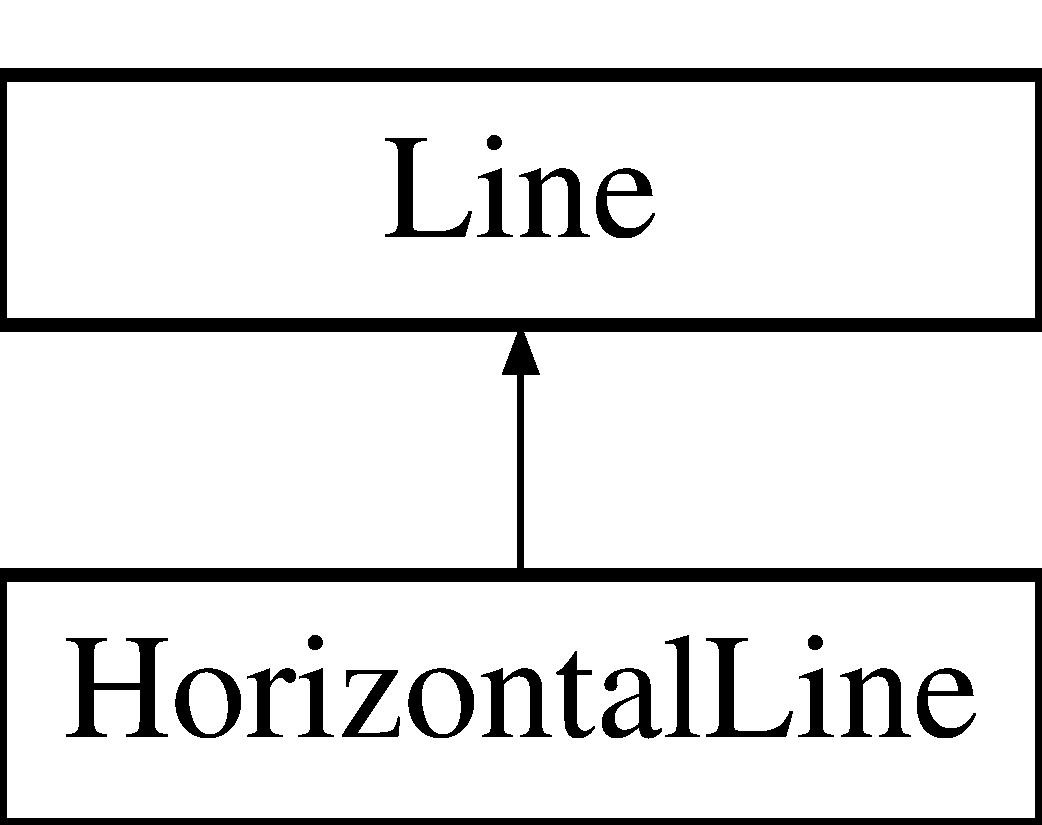
\includegraphics[height=2.000000cm]{classHorizontalLine}
\end{center}
\end{figure}
\subsection*{\-Public \-Member \-Functions}
\begin{DoxyCompactItemize}
\item 
\hyperlink{classHorizontalLine_ad74caf3817002a674c7e8e813bb3fb73}{\-Horizontal\-Line} (\hyperlink{classBox}{\-Box} $\ast$above, \hyperlink{classBox}{\-Box} $\ast$under, \-Q\-Object $\ast$parent=0)
\begin{DoxyCompactList}\small\item\em \-Default constructor. \end{DoxyCompactList}\item 
virtual \hyperlink{classHorizontalLine_a466f8a4e47a315d901cef8b3b1856366}{$\sim$\-Horizontal\-Line} ()
\begin{DoxyCompactList}\small\item\em \-Destructor. \end{DoxyCompactList}\item 
void \hyperlink{classHorizontalLine_ae4b1b9f4b9de1e4393868675813fbf8c}{turn\-Grey} ()
\begin{DoxyCompactList}\small\item\em \-Makes the line grey. \end{DoxyCompactList}\item 
bool \hyperlink{classHorizontalLine_aefd796758e374952b730268387f134e6}{play\-Turn} (bool user\-Turn)
\begin{DoxyCompactList}\small\item\em \-Called when a line is selected. \end{DoxyCompactList}\item 
\hyperlink{classBox}{\-Box} $\ast$ \hyperlink{classHorizontalLine_ad2289edae1e1ce26630d0215578ae5b6}{get\-Above} () const 
\begin{DoxyCompactList}\small\item\em \-Gets the box above the line. \end{DoxyCompactList}\item 
\hyperlink{classBox}{\-Box} $\ast$ \hyperlink{classHorizontalLine_aafd04b01e9a589e429b3bfd500c1ff2e}{get\-Under} () const 
\begin{DoxyCompactList}\small\item\em \-Gets the box under the line. \end{DoxyCompactList}\end{DoxyCompactItemize}


\subsection{\-Constructor \& \-Destructor \-Documentation}
\hypertarget{classHorizontalLine_ad74caf3817002a674c7e8e813bb3fb73}{\index{\-Horizontal\-Line@{\-Horizontal\-Line}!\-Horizontal\-Line@{\-Horizontal\-Line}}
\index{\-Horizontal\-Line@{\-Horizontal\-Line}!HorizontalLine@{\-Horizontal\-Line}}
\subsubsection[{\-Horizontal\-Line}]{\setlength{\rightskip}{0pt plus 5cm}{\bf \-Horizontal\-Line\-::\-Horizontal\-Line} (
\begin{DoxyParamCaption}
\item[{{\bf \-Box} $\ast$}]{above, }
\item[{{\bf \-Box} $\ast$}]{under, }
\item[{\-Q\-Object $\ast$}]{parent = {\ttfamily 0}}
\end{DoxyParamCaption}
)\hspace{0.3cm}{\ttfamily  \mbox{[}explicit\mbox{]}}}}\label{classHorizontalLine_ad74caf3817002a674c7e8e813bb3fb73}


\-Default constructor. 


\begin{DoxyParams}{\-Parameters}
{\em above} & \hyperlink{classBox}{\-Box} above line \\
\hline
{\em under} & \hyperlink{classBox}{\-Box} under line\\
\hline
\end{DoxyParams}
\-Sets \hyperlink{classHorizontalLine}{\-Horizontal\-Line} properties. \hypertarget{classHorizontalLine_a466f8a4e47a315d901cef8b3b1856366}{\index{\-Horizontal\-Line@{\-Horizontal\-Line}!$\sim$\-Horizontal\-Line@{$\sim$\-Horizontal\-Line}}
\index{$\sim$\-Horizontal\-Line@{$\sim$\-Horizontal\-Line}!HorizontalLine@{\-Horizontal\-Line}}
\subsubsection[{$\sim$\-Horizontal\-Line}]{\setlength{\rightskip}{0pt plus 5cm}{\bf \-Horizontal\-Line\-::$\sim$\-Horizontal\-Line} (
\begin{DoxyParamCaption}
{}
\end{DoxyParamCaption}
)\hspace{0.3cm}{\ttfamily  \mbox{[}virtual\mbox{]}}}}\label{classHorizontalLine_a466f8a4e47a315d901cef8b3b1856366}


\-Destructor. 

\-Frees allocated memory. 

\subsection{\-Member \-Function \-Documentation}
\hypertarget{classHorizontalLine_ad2289edae1e1ce26630d0215578ae5b6}{\index{\-Horizontal\-Line@{\-Horizontal\-Line}!get\-Above@{get\-Above}}
\index{get\-Above@{get\-Above}!HorizontalLine@{\-Horizontal\-Line}}
\subsubsection[{get\-Above}]{\setlength{\rightskip}{0pt plus 5cm}{\bf \-Box} $\ast$ {\bf \-Horizontal\-Line\-::get\-Above} (
\begin{DoxyParamCaption}
{}
\end{DoxyParamCaption}
) const}}\label{classHorizontalLine_ad2289edae1e1ce26630d0215578ae5b6}


\-Gets the box above the line. 

\begin{DoxyReturn}{\-Returns}
box above the line
\end{DoxyReturn}
\-Returns the box above the line. \hypertarget{classHorizontalLine_aafd04b01e9a589e429b3bfd500c1ff2e}{\index{\-Horizontal\-Line@{\-Horizontal\-Line}!get\-Under@{get\-Under}}
\index{get\-Under@{get\-Under}!HorizontalLine@{\-Horizontal\-Line}}
\subsubsection[{get\-Under}]{\setlength{\rightskip}{0pt plus 5cm}{\bf \-Box} $\ast$ {\bf \-Horizontal\-Line\-::get\-Under} (
\begin{DoxyParamCaption}
{}
\end{DoxyParamCaption}
) const}}\label{classHorizontalLine_aafd04b01e9a589e429b3bfd500c1ff2e}


\-Gets the box under the line. 

\begin{DoxyReturn}{\-Returns}
box under the line
\end{DoxyReturn}
\-Returns the box under the line. \hypertarget{classHorizontalLine_aefd796758e374952b730268387f134e6}{\index{\-Horizontal\-Line@{\-Horizontal\-Line}!play\-Turn@{play\-Turn}}
\index{play\-Turn@{play\-Turn}!HorizontalLine@{\-Horizontal\-Line}}
\subsubsection[{play\-Turn}]{\setlength{\rightskip}{0pt plus 5cm}bool {\bf \-Horizontal\-Line\-::play\-Turn} (
\begin{DoxyParamCaption}
\item[{bool}]{user\-Turn}
\end{DoxyParamCaption}
)\hspace{0.3cm}{\ttfamily  \mbox{[}virtual\mbox{]}}}}\label{classHorizontalLine_aefd796758e374952b730268387f134e6}


\-Called when a line is selected. 


\begin{DoxyParams}{\-Parameters}
{\em user\-Turn} & \-Whether it is the user's turn \\
\hline
\end{DoxyParams}
\begin{DoxyReturn}{\-Returns}
\-Whether it is still the player's turn
\end{DoxyReturn}
\-Called when a line is drawn. \-Returns whether it is still the same player's turn. 

\-Implements \hyperlink{classLine_adb2af7d5815c082d2c7864a86af27b14}{\-Line}.

\hypertarget{classHorizontalLine_ae4b1b9f4b9de1e4393868675813fbf8c}{\index{\-Horizontal\-Line@{\-Horizontal\-Line}!turn\-Grey@{turn\-Grey}}
\index{turn\-Grey@{turn\-Grey}!HorizontalLine@{\-Horizontal\-Line}}
\subsubsection[{turn\-Grey}]{\setlength{\rightskip}{0pt plus 5cm}void {\bf \-Horizontal\-Line\-::turn\-Grey} (
\begin{DoxyParamCaption}
{}
\end{DoxyParamCaption}
)\hspace{0.3cm}{\ttfamily  \mbox{[}virtual\mbox{]}}}}\label{classHorizontalLine_ae4b1b9f4b9de1e4393868675813fbf8c}


\-Makes the line grey. 

\-Changes the object image to make it grey. 

\-Implements \hyperlink{classLine_a63f54b0b50d2c6db91fc7d97c15433b1}{\-Line}.



\-The documentation for this class was generated from the following files\-:\begin{DoxyCompactItemize}
\item 
game3/\hyperlink{horizontalline_8h}{horizontalline.\-h}\item 
game3/\hyperlink{horizontalline_8cpp}{horizontalline.\-cpp}\end{DoxyCompactItemize}

\hypertarget{classLine}{\section{\-Line \-Class \-Reference}
\label{classLine}\index{\-Line@{\-Line}}
}
\-Inheritance diagram for \-Line\-:\begin{figure}[H]
\begin{center}
\leavevmode
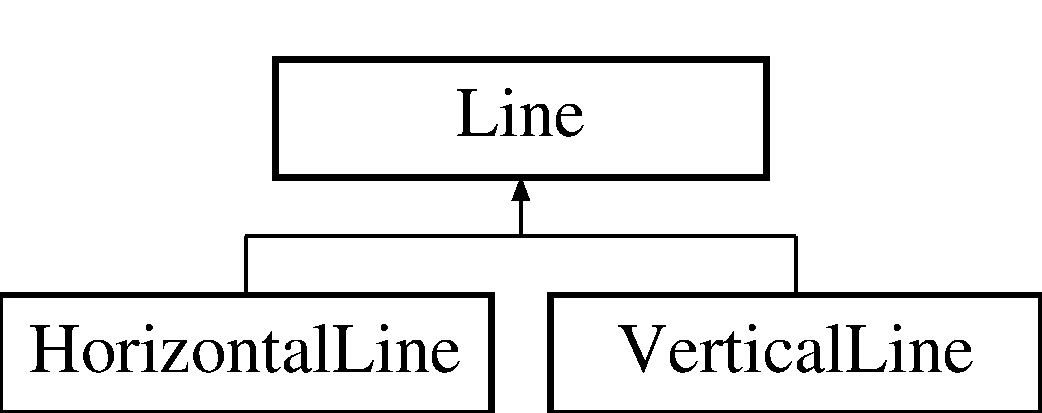
\includegraphics[height=2.000000cm]{classLine}
\end{center}
\end{figure}
\subsection*{\-Public \-Member \-Functions}
\begin{DoxyCompactItemize}
\item 
\hyperlink{classLine_a556ea343ae2c6118ed775f99b1c1bd0a}{\-Line} (bool \hyperlink{classLine_a799c03e48bd560a9f6c0b2b729e38855}{is\-Horizontal}, \-Q\-Object $\ast$parent=0)
\begin{DoxyCompactList}\small\item\em \-Default constructor. \end{DoxyCompactList}\item 
\hypertarget{classLine_a63f54b0b50d2c6db91fc7d97c15433b1}{virtual void \hyperlink{classLine_a63f54b0b50d2c6db91fc7d97c15433b1}{turn\-Grey} ()=0}\label{classLine_a63f54b0b50d2c6db91fc7d97c15433b1}

\begin{DoxyCompactList}\small\item\em \-Makes the line grey. \end{DoxyCompactList}\item 
void \hyperlink{classLine_aac8ab0980da0a3db6e4991e734462193}{mouse\-Press\-Event} (\-Q\-Graphics\-Scene\-Mouse\-Event $\ast$event)
\begin{DoxyCompactList}\small\item\em \-Called when the user clicks on the line. \end{DoxyCompactList}\item 
virtual bool \hyperlink{classLine_adb2af7d5815c082d2c7864a86af27b14}{play\-Turn} (bool user\-Turn)=0
\begin{DoxyCompactList}\small\item\em \-Called when a line is selected. \end{DoxyCompactList}\item 
bool \hyperlink{classLine_a1adc846d2872638610850cc27e325317}{is\-Drawn} () const 
\begin{DoxyCompactList}\small\item\em \-Returns whether the line has been drawn already. \end{DoxyCompactList}\item 
\hypertarget{classLine_ab6265993bf5acbc28830181c3e712f10}{void \hyperlink{classLine_ab6265993bf5acbc28830181c3e712f10}{draw} ()}\label{classLine_ab6265993bf5acbc28830181c3e712f10}

\begin{DoxyCompactList}\small\item\em \-Sets the line as drawn. \end{DoxyCompactList}\item 
bool \hyperlink{classLine_a799c03e48bd560a9f6c0b2b729e38855}{is\-Horizontal} () const 
\begin{DoxyCompactList}\small\item\em \-Returns whether the line is horizontal or vertical. \end{DoxyCompactList}\end{DoxyCompactItemize}


\subsection{\-Constructor \& \-Destructor \-Documentation}
\hypertarget{classLine_a556ea343ae2c6118ed775f99b1c1bd0a}{\index{\-Line@{\-Line}!\-Line@{\-Line}}
\index{\-Line@{\-Line}!Line@{\-Line}}
\subsubsection[{\-Line}]{\setlength{\rightskip}{0pt plus 5cm}{\bf \-Line\-::\-Line} (
\begin{DoxyParamCaption}
\item[{bool}]{is\-Horizontal, }
\item[{\-Q\-Object $\ast$}]{parent = {\ttfamily 0}}
\end{DoxyParamCaption}
)\hspace{0.3cm}{\ttfamily  \mbox{[}explicit\mbox{]}}}}\label{classLine_a556ea343ae2c6118ed775f99b1c1bd0a}


\-Default constructor. 


\begin{DoxyParams}{\-Parameters}
{\em is\-Horizontal} & \-Whether the line is horizontal or not (vertical)\\
\hline
\end{DoxyParams}
\-Initializes the object and marks it as not drawn. 

\subsection{\-Member \-Function \-Documentation}
\hypertarget{classLine_a1adc846d2872638610850cc27e325317}{\index{\-Line@{\-Line}!is\-Drawn@{is\-Drawn}}
\index{is\-Drawn@{is\-Drawn}!Line@{\-Line}}
\subsubsection[{is\-Drawn}]{\setlength{\rightskip}{0pt plus 5cm}bool {\bf \-Line\-::is\-Drawn} (
\begin{DoxyParamCaption}
{}
\end{DoxyParamCaption}
) const}}\label{classLine_a1adc846d2872638610850cc27e325317}


\-Returns whether the line has been drawn already. 

\begin{DoxyReturn}{\-Returns}
\-Whether the line has been drawn already 
\end{DoxyReturn}
\hypertarget{classLine_a799c03e48bd560a9f6c0b2b729e38855}{\index{\-Line@{\-Line}!is\-Horizontal@{is\-Horizontal}}
\index{is\-Horizontal@{is\-Horizontal}!Line@{\-Line}}
\subsubsection[{is\-Horizontal}]{\setlength{\rightskip}{0pt plus 5cm}bool {\bf \-Line\-::is\-Horizontal} (
\begin{DoxyParamCaption}
{}
\end{DoxyParamCaption}
) const}}\label{classLine_a799c03e48bd560a9f6c0b2b729e38855}


\-Returns whether the line is horizontal or vertical. 

\begin{DoxyReturn}{\-Returns}
\-Whether the line is horizontal
\end{DoxyReturn}
\-Returns whether the line is horizontal or vertical \hypertarget{classLine_aac8ab0980da0a3db6e4991e734462193}{\index{\-Line@{\-Line}!mouse\-Press\-Event@{mouse\-Press\-Event}}
\index{mouse\-Press\-Event@{mouse\-Press\-Event}!Line@{\-Line}}
\subsubsection[{mouse\-Press\-Event}]{\setlength{\rightskip}{0pt plus 5cm}void {\bf \-Line\-::mouse\-Press\-Event} (
\begin{DoxyParamCaption}
\item[{\-Q\-Graphics\-Scene\-Mouse\-Event $\ast$}]{event}
\end{DoxyParamCaption}
)}}\label{classLine_aac8ab0980da0a3db6e4991e734462193}


\-Called when the user clicks on the line. 

\-Called when the user clicks on the line. \-The function changes the states of corresponding lines and boxes. \-It then checks for a win. \hypertarget{classLine_adb2af7d5815c082d2c7864a86af27b14}{\index{\-Line@{\-Line}!play\-Turn@{play\-Turn}}
\index{play\-Turn@{play\-Turn}!Line@{\-Line}}
\subsubsection[{play\-Turn}]{\setlength{\rightskip}{0pt plus 5cm}virtual bool {\bf \-Line\-::play\-Turn} (
\begin{DoxyParamCaption}
\item[{bool}]{user\-Turn}
\end{DoxyParamCaption}
)\hspace{0.3cm}{\ttfamily  \mbox{[}pure virtual\mbox{]}}}}\label{classLine_adb2af7d5815c082d2c7864a86af27b14}


\-Called when a line is selected. 


\begin{DoxyParams}{\-Parameters}
{\em user\-Turn} & \-Whether it is the user's turn \\
\hline
\end{DoxyParams}
\begin{DoxyReturn}{\-Returns}
\-Whether it is still the player's turn 
\end{DoxyReturn}


\-Implemented in \hyperlink{classHorizontalLine_aefd796758e374952b730268387f134e6}{\-Horizontal\-Line}, and \hyperlink{classVerticalLine_ac90ef61324404c12668c73dc5567dc11}{\-Vertical\-Line}.



\-The documentation for this class was generated from the following files\-:\begin{DoxyCompactItemize}
\item 
game3/\hyperlink{line_8h}{line.\-h}\item 
game3/\hyperlink{line_8cpp}{line.\-cpp}\end{DoxyCompactItemize}

\hypertarget{classMainWidget}{\section{\-Main\-Widget \-Class \-Reference}
\label{classMainWidget}\index{\-Main\-Widget@{\-Main\-Widget}}
}
\subsection*{\-Public \-Slots}
\begin{DoxyCompactItemize}
\item 
\hypertarget{classMainWidget_a438fbcb90c6dcb9301d70c5b34d98900}{void \hyperlink{classMainWidget_a438fbcb90c6dcb9301d70c5b34d98900}{go\-To\-Game\-Selection} ()}\label{classMainWidget_a438fbcb90c6dcb9301d70c5b34d98900}

\begin{DoxyCompactList}\small\item\em \-Slot that closes widget and opens the game selection menu. \end{DoxyCompactList}\end{DoxyCompactItemize}
\subsection*{\-Public \-Member \-Functions}
\begin{DoxyCompactItemize}
\item 
\hyperlink{classMainWidget_a326fee5088b7cebaa102ed5332dd59ee}{\-Main\-Widget} (\-Q\-Widget $\ast$parent=0)
\begin{DoxyCompactList}\small\item\em \-Default constructor. \end{DoxyCompactList}\item 
virtual \hyperlink{classMainWidget_add21c63f8e799303a21a69da3d288c2f}{$\sim$\-Main\-Widget} ()
\begin{DoxyCompactList}\small\item\em \-Destructor. \end{DoxyCompactList}\end{DoxyCompactItemize}


\subsection{\-Constructor \& \-Destructor \-Documentation}
\hypertarget{classMainWidget_a326fee5088b7cebaa102ed5332dd59ee}{\index{\-Main\-Widget@{\-Main\-Widget}!\-Main\-Widget@{\-Main\-Widget}}
\index{\-Main\-Widget@{\-Main\-Widget}!MainWidget@{\-Main\-Widget}}
\subsubsection[{\-Main\-Widget}]{\setlength{\rightskip}{0pt plus 5cm}{\bf \-Main\-Widget\-::\-Main\-Widget} (
\begin{DoxyParamCaption}
\item[{\-Q\-Widget $\ast$}]{parent = {\ttfamily 0}}
\end{DoxyParamCaption}
)\hspace{0.3cm}{\ttfamily  \mbox{[}explicit\mbox{]}}}}\label{classMainWidget_a326fee5088b7cebaa102ed5332dd59ee}


\-Default constructor. 

\-Initializes all buttons, input fields and labels and shows them on the screen. \hypertarget{classMainWidget_add21c63f8e799303a21a69da3d288c2f}{\index{\-Main\-Widget@{\-Main\-Widget}!$\sim$\-Main\-Widget@{$\sim$\-Main\-Widget}}
\index{$\sim$\-Main\-Widget@{$\sim$\-Main\-Widget}!MainWidget@{\-Main\-Widget}}
\subsubsection[{$\sim$\-Main\-Widget}]{\setlength{\rightskip}{0pt plus 5cm}{\bf \-Main\-Widget\-::$\sim$\-Main\-Widget} (
\begin{DoxyParamCaption}
{}
\end{DoxyParamCaption}
)\hspace{0.3cm}{\ttfamily  \mbox{[}virtual\mbox{]}}}}\label{classMainWidget_add21c63f8e799303a21a69da3d288c2f}


\-Destructor. 

\-Frees allocated memory. 

\-The documentation for this class was generated from the following files\-:\begin{DoxyCompactItemize}
\item 
gui/\hyperlink{mainwidget_8h}{mainwidget.\-h}\item 
gui/\hyperlink{mainwidget_8cpp}{mainwidget.\-cpp}\end{DoxyCompactItemize}

\hypertarget{classMyAccount}{\section{\-My\-Account \-Class \-Reference}
\label{classMyAccount}\index{\-My\-Account@{\-My\-Account}}
}
\subsection*{\-Public \-Slots}
\begin{DoxyCompactItemize}
\item 
void \hyperlink{classMyAccount_a9dc73e591e529adb0628291d2efe9dad}{go\-To\-Games} ()
\begin{DoxyCompactList}\small\item\em \-Goes back to the games selection menu. \end{DoxyCompactList}\item 
void \hyperlink{classMyAccount_aad84a64cbf944d18ecc14ca628e7336e}{show\-Game\-Graph} (int gamenb)
\begin{DoxyCompactList}\small\item\em \-Displays the graph of the selected game. \end{DoxyCompactList}\end{DoxyCompactItemize}
\subsection*{\-Public \-Member \-Functions}
\begin{DoxyCompactItemize}
\item 
\hyperlink{classMyAccount_a1ce3bceec0bd63885b8f85890128f23c}{\-My\-Account} (\-Q\-Widget $\ast$parent=0)
\begin{DoxyCompactList}\small\item\em \-Default constructor. \end{DoxyCompactList}\item 
virtual \hyperlink{classMyAccount_a68bdda0b0bd909f5e99d87118cf55ebd}{$\sim$\-My\-Account} ()
\begin{DoxyCompactList}\small\item\em \-Destructor. \end{DoxyCompactList}\end{DoxyCompactItemize}


\subsection{\-Constructor \& \-Destructor \-Documentation}
\hypertarget{classMyAccount_a1ce3bceec0bd63885b8f85890128f23c}{\index{\-My\-Account@{\-My\-Account}!\-My\-Account@{\-My\-Account}}
\index{\-My\-Account@{\-My\-Account}!MyAccount@{\-My\-Account}}
\subsubsection[{\-My\-Account}]{\setlength{\rightskip}{0pt plus 5cm}{\bf \-My\-Account\-::\-My\-Account} (
\begin{DoxyParamCaption}
\item[{\-Q\-Widget $\ast$}]{parent = {\ttfamily 0}}
\end{DoxyParamCaption}
)\hspace{0.3cm}{\ttfamily  \mbox{[}explicit\mbox{]}}}}\label{classMyAccount_a1ce3bceec0bd63885b8f85890128f23c}


\-Default constructor. 

\-Initializes all buttons and labels and shows them on the game selection menu. \hypertarget{classMyAccount_a68bdda0b0bd909f5e99d87118cf55ebd}{\index{\-My\-Account@{\-My\-Account}!$\sim$\-My\-Account@{$\sim$\-My\-Account}}
\index{$\sim$\-My\-Account@{$\sim$\-My\-Account}!MyAccount@{\-My\-Account}}
\subsubsection[{$\sim$\-My\-Account}]{\setlength{\rightskip}{0pt plus 5cm}{\bf \-My\-Account\-::$\sim$\-My\-Account} (
\begin{DoxyParamCaption}
{}
\end{DoxyParamCaption}
)\hspace{0.3cm}{\ttfamily  \mbox{[}virtual\mbox{]}}}}\label{classMyAccount_a68bdda0b0bd909f5e99d87118cf55ebd}


\-Destructor. 

\-Frees allocated memory. 

\subsection{\-Member \-Function \-Documentation}
\hypertarget{classMyAccount_a9dc73e591e529adb0628291d2efe9dad}{\index{\-My\-Account@{\-My\-Account}!go\-To\-Games@{go\-To\-Games}}
\index{go\-To\-Games@{go\-To\-Games}!MyAccount@{\-My\-Account}}
\subsubsection[{go\-To\-Games}]{\setlength{\rightskip}{0pt plus 5cm}void {\bf \-My\-Account\-::go\-To\-Games} (
\begin{DoxyParamCaption}
{}
\end{DoxyParamCaption}
)\hspace{0.3cm}{\ttfamily  \mbox{[}slot\mbox{]}}}}\label{classMyAccount_a9dc73e591e529adb0628291d2efe9dad}


\-Goes back to the games selection menu. 

\-Takes the user back to the game selection menu. \-Called when the user clicks the corresponding button. \hypertarget{classMyAccount_aad84a64cbf944d18ecc14ca628e7336e}{\index{\-My\-Account@{\-My\-Account}!show\-Game\-Graph@{show\-Game\-Graph}}
\index{show\-Game\-Graph@{show\-Game\-Graph}!MyAccount@{\-My\-Account}}
\subsubsection[{show\-Game\-Graph}]{\setlength{\rightskip}{0pt plus 5cm}void {\bf \-My\-Account\-::show\-Game\-Graph} (
\begin{DoxyParamCaption}
\item[{int}]{gamenb}
\end{DoxyParamCaption}
)\hspace{0.3cm}{\ttfamily  \mbox{[}slot\mbox{]}}}}\label{classMyAccount_aad84a64cbf944d18ecc14ca628e7336e}


\-Displays the graph of the selected game. 


\begin{DoxyParams}{\-Parameters}
{\em gamenb} & \-The number of the game \\
\hline
\end{DoxyParams}


\-The documentation for this class was generated from the following files\-:\begin{DoxyCompactItemize}
\item 
account/\hyperlink{myaccount_8h}{myaccount.\-h}\item 
account/\hyperlink{myaccount_8cpp}{myaccount.\-cpp}\end{DoxyCompactItemize}

\hypertarget{classShaunGamesTest}{\section{\-Shaun\-Games\-Test \-Class \-Reference}
\label{classShaunGamesTest}\index{\-Shaun\-Games\-Test@{\-Shaun\-Games\-Test}}
}
\subsection*{\-Public \-Member \-Functions}
\begin{DoxyCompactItemize}
\item 
\hypertarget{classShaunGamesTest_ac28823579a80e51eba218cc5c14ad83a}{void {\bfseries set\-Up} ()}\label{classShaunGamesTest_ac28823579a80e51eba218cc5c14ad83a}

\item 
\hypertarget{classShaunGamesTest_a4eac20bf37edcb06406385e6d34d5a30}{void {\bfseries tear\-Down} ()}\label{classShaunGamesTest_a4eac20bf37edcb06406385e6d34d5a30}

\end{DoxyCompactItemize}
\subsection*{\-Protected \-Member \-Functions}
\begin{DoxyCompactItemize}
\item 
\hypertarget{classShaunGamesTest_a942c9a600c86425c5a366138d7055956}{void {\bfseries to\-Radians\-Test} ()}\label{classShaunGamesTest_a942c9a600c86425c5a366138d7055956}

\item 
\hypertarget{classShaunGamesTest_a48473265c196e8dc38e0d0c9c66fd3c0}{void {\bfseries get\-Random\-Sheep\-Number\-Test} ()}\label{classShaunGamesTest_a48473265c196e8dc38e0d0c9c66fd3c0}

\end{DoxyCompactItemize}


\-The documentation for this class was generated from the following files\-:\begin{DoxyCompactItemize}
\item 
tests/\-Shaun\-Games\-Test.\-h\item 
tests/\-Shaun\-Games\-Test.\-cpp\end{DoxyCompactItemize}

\hypertarget{classSheep1}{\section{\-Sheep1 \-Class \-Reference}
\label{classSheep1}\index{\-Sheep1@{\-Sheep1}}
}
\subsection*{\-Public \-Slots}
\begin{DoxyCompactItemize}
\item 
void \hyperlink{classSheep1_a1d152e5c8c94201d057c40a63f7ec33b}{fired\-Move} ()
\begin{DoxyCompactList}\small\item\em \-Moves the sheep in the direction of the firing. \end{DoxyCompactList}\end{DoxyCompactItemize}
\subsection*{\-Public \-Member \-Functions}
\begin{DoxyCompactItemize}
\item 
\hyperlink{classSheep1_ac421bb46b209fc0c2a198d91a07ebfff}{\-Sheep1} (int number, bool in\-Line, \-Q\-Object $\ast$parent=0)
\begin{DoxyCompactList}\small\item\em \-Constructor. \end{DoxyCompactList}\item 
virtual \hyperlink{classSheep1_a2622bc6b1343023ec74412b811f6531c}{$\sim$\-Sheep1} ()
\begin{DoxyCompactList}\small\item\em \-Destructor. \end{DoxyCompactList}\item 
double \hyperlink{classSheep1_ab0e6c2a234909380c689e8588d7f6cfb}{get\-Angle} () const 
\begin{DoxyCompactList}\small\item\em \-Gets the angle of the sheep in degrees. \end{DoxyCompactList}\item 
void \hyperlink{classSheep1_a1644fdc3958aa506c792e5bf0e1ec964}{set\-Angle} (double angle)
\begin{DoxyCompactList}\small\item\em \-Sets the angle of the sheep in degrees. \end{DoxyCompactList}\item 
bool \hyperlink{classSheep1_a5bfd6e9f199c39fbc6daa3a679905653}{is\-In\-Line} () const 
\begin{DoxyCompactList}\small\item\em \-Checks whether the sheep is part of the moving line. \end{DoxyCompactList}\item 
void \hyperlink{classSheep1_ad5902cd1b715217e0bff1803c67e7184}{set\-In\-Line} (bool in\-Line)
\begin{DoxyCompactList}\small\item\em \-Changes the status of the sheep as in or out of the moving line. \end{DoxyCompactList}\item 
void \hyperlink{classSheep1_abe21e78851d4df2fc7e989c7f54121fb}{fire} (double angle)
\begin{DoxyCompactList}\small\item\em \-Fires the sheep in a straight line. \end{DoxyCompactList}\item 
void \hyperlink{classSheep1_af82457038ce2bdae2cb85b09e093b8fe}{move\-In\-Line} (double distance)
\begin{DoxyCompactList}\small\item\em \-Moves the sheep in line by given distance. \end{DoxyCompactList}\item 
double \hyperlink{classSheep1_aa25f6b89d1a6de8f0c0afd7885176777}{in\-Line\-Distance\-To} (const \hyperlink{classSheep1}{\-Sheep1} $\ast$other) const 
\begin{DoxyCompactList}\small\item\em \-Returns the in-\/line distance between object and given sheep. \end{DoxyCompactList}\item 
int \hyperlink{classSheep1_a67846c27af775696140663a6b39da7d2}{get\-Number} () const 
\begin{DoxyCompactList}\small\item\em \-Returns the sheep number. \end{DoxyCompactList}\end{DoxyCompactItemize}
\subsection*{\-Static \-Public \-Member \-Functions}
\begin{DoxyCompactItemize}
\item 
static int \hyperlink{classSheep1_aa2a9a9c68c9a18a1eeaa732badfcea82}{get\-Random\-Sheep\-Number} ()
\begin{DoxyCompactList}\small\item\em \-Returns a number between 1 and 9. \end{DoxyCompactList}\end{DoxyCompactItemize}


\subsection{\-Constructor \& \-Destructor \-Documentation}
\hypertarget{classSheep1_ac421bb46b209fc0c2a198d91a07ebfff}{\index{\-Sheep1@{\-Sheep1}!\-Sheep1@{\-Sheep1}}
\index{\-Sheep1@{\-Sheep1}!Sheep1@{\-Sheep1}}
\subsubsection[{\-Sheep1}]{\setlength{\rightskip}{0pt plus 5cm}{\bf \-Sheep1\-::\-Sheep1} (
\begin{DoxyParamCaption}
\item[{int}]{number, }
\item[{bool}]{in\-Line, }
\item[{\-Q\-Object $\ast$}]{parent = {\ttfamily 0}}
\end{DoxyParamCaption}
)\hspace{0.3cm}{\ttfamily  \mbox{[}explicit\mbox{]}}}}\label{classSheep1_ac421bb46b209fc0c2a198d91a07ebfff}


\-Constructor. 


\begin{DoxyParams}{\-Parameters}
{\em number} & \-Sheep number \\
\hline
{\em in\-Line} & \-Whether sheep is in line\\
\hline
\end{DoxyParams}
\-Sets the properties of the sheep. \hypertarget{classSheep1_a2622bc6b1343023ec74412b811f6531c}{\index{\-Sheep1@{\-Sheep1}!$\sim$\-Sheep1@{$\sim$\-Sheep1}}
\index{$\sim$\-Sheep1@{$\sim$\-Sheep1}!Sheep1@{\-Sheep1}}
\subsubsection[{$\sim$\-Sheep1}]{\setlength{\rightskip}{0pt plus 5cm}{\bf \-Sheep1\-::$\sim$\-Sheep1} (
\begin{DoxyParamCaption}
{}
\end{DoxyParamCaption}
)\hspace{0.3cm}{\ttfamily  \mbox{[}virtual\mbox{]}}}}\label{classSheep1_a2622bc6b1343023ec74412b811f6531c}


\-Destructor. 

\-Frees allocated memory. 

\subsection{\-Member \-Function \-Documentation}
\hypertarget{classSheep1_abe21e78851d4df2fc7e989c7f54121fb}{\index{\-Sheep1@{\-Sheep1}!fire@{fire}}
\index{fire@{fire}!Sheep1@{\-Sheep1}}
\subsubsection[{fire}]{\setlength{\rightskip}{0pt plus 5cm}void {\bf \-Sheep1\-::fire} (
\begin{DoxyParamCaption}
\item[{double}]{angle}
\end{DoxyParamCaption}
)}}\label{classSheep1_abe21e78851d4df2fc7e989c7f54121fb}


\-Fires the sheep in a straight line. 


\begin{DoxyParams}{\-Parameters}
{\em angle} & \-Angle at which to fire the sheep\\
\hline
\end{DoxyParams}
\-Fires sheep at an angle. \-Called when the user fires the cannon. \hypertarget{classSheep1_a1d152e5c8c94201d057c40a63f7ec33b}{\index{\-Sheep1@{\-Sheep1}!fired\-Move@{fired\-Move}}
\index{fired\-Move@{fired\-Move}!Sheep1@{\-Sheep1}}
\subsubsection[{fired\-Move}]{\setlength{\rightskip}{0pt plus 5cm}void {\bf \-Sheep1\-::fired\-Move} (
\begin{DoxyParamCaption}
{}
\end{DoxyParamCaption}
)\hspace{0.3cm}{\ttfamily  \mbox{[}slot\mbox{]}}}}\label{classSheep1_a1d152e5c8c94201d057c40a63f7ec33b}


\-Moves the sheep in the direction of the firing. 

\-Moves the sheep in the distance of the firing of the cannon. \hypertarget{classSheep1_ab0e6c2a234909380c689e8588d7f6cfb}{\index{\-Sheep1@{\-Sheep1}!get\-Angle@{get\-Angle}}
\index{get\-Angle@{get\-Angle}!Sheep1@{\-Sheep1}}
\subsubsection[{get\-Angle}]{\setlength{\rightskip}{0pt plus 5cm}double {\bf \-Sheep1\-::get\-Angle} (
\begin{DoxyParamCaption}
{}
\end{DoxyParamCaption}
) const}}\label{classSheep1_ab0e6c2a234909380c689e8588d7f6cfb}


\-Gets the angle of the sheep in degrees. 

\begin{DoxyReturn}{\-Returns}
\-The angle of the sheep in the circle 
\end{DoxyReturn}
\hypertarget{classSheep1_a67846c27af775696140663a6b39da7d2}{\index{\-Sheep1@{\-Sheep1}!get\-Number@{get\-Number}}
\index{get\-Number@{get\-Number}!Sheep1@{\-Sheep1}}
\subsubsection[{get\-Number}]{\setlength{\rightskip}{0pt plus 5cm}int {\bf \-Sheep1\-::get\-Number} (
\begin{DoxyParamCaption}
{}
\end{DoxyParamCaption}
) const}}\label{classSheep1_a67846c27af775696140663a6b39da7d2}


\-Returns the sheep number. 

\begin{DoxyReturn}{\-Returns}
\-Sheep number 
\end{DoxyReturn}
\hypertarget{classSheep1_aa2a9a9c68c9a18a1eeaa732badfcea82}{\index{\-Sheep1@{\-Sheep1}!get\-Random\-Sheep\-Number@{get\-Random\-Sheep\-Number}}
\index{get\-Random\-Sheep\-Number@{get\-Random\-Sheep\-Number}!Sheep1@{\-Sheep1}}
\subsubsection[{get\-Random\-Sheep\-Number}]{\setlength{\rightskip}{0pt plus 5cm}int {\bf \-Sheep1\-::get\-Random\-Sheep\-Number} (
\begin{DoxyParamCaption}
{}
\end{DoxyParamCaption}
)\hspace{0.3cm}{\ttfamily  \mbox{[}static\mbox{]}}}}\label{classSheep1_aa2a9a9c68c9a18a1eeaa732badfcea82}


\-Returns a number between 1 and 9. 

\begin{DoxyReturn}{\-Returns}
\-Number between 1 and 9
\end{DoxyReturn}
\-Returns a random sheep number between 1 and 9. \hypertarget{classSheep1_aa25f6b89d1a6de8f0c0afd7885176777}{\index{\-Sheep1@{\-Sheep1}!in\-Line\-Distance\-To@{in\-Line\-Distance\-To}}
\index{in\-Line\-Distance\-To@{in\-Line\-Distance\-To}!Sheep1@{\-Sheep1}}
\subsubsection[{in\-Line\-Distance\-To}]{\setlength{\rightskip}{0pt plus 5cm}double {\bf \-Sheep1\-::in\-Line\-Distance\-To} (
\begin{DoxyParamCaption}
\item[{const {\bf \-Sheep1} $\ast$}]{other}
\end{DoxyParamCaption}
) const}}\label{classSheep1_aa25f6b89d1a6de8f0c0afd7885176777}


\-Returns the in-\/line distance between object and given sheep. 


\begin{DoxyParams}{\-Parameters}
{\em other} & \-Other sheep \\
\hline
\end{DoxyParams}
\begin{DoxyReturn}{\-Returns}
\-Distance in pixels
\end{DoxyReturn}
\-Calculates the distance between the two in-\/line sheep. \hypertarget{classSheep1_a5bfd6e9f199c39fbc6daa3a679905653}{\index{\-Sheep1@{\-Sheep1}!is\-In\-Line@{is\-In\-Line}}
\index{is\-In\-Line@{is\-In\-Line}!Sheep1@{\-Sheep1}}
\subsubsection[{is\-In\-Line}]{\setlength{\rightskip}{0pt plus 5cm}bool {\bf \-Sheep1\-::is\-In\-Line} (
\begin{DoxyParamCaption}
{}
\end{DoxyParamCaption}
) const}}\label{classSheep1_a5bfd6e9f199c39fbc6daa3a679905653}


\-Checks whether the sheep is part of the moving line. 

\begin{DoxyReturn}{\-Returns}
\-Whether sheep is in line 
\end{DoxyReturn}
\hypertarget{classSheep1_af82457038ce2bdae2cb85b09e093b8fe}{\index{\-Sheep1@{\-Sheep1}!move\-In\-Line@{move\-In\-Line}}
\index{move\-In\-Line@{move\-In\-Line}!Sheep1@{\-Sheep1}}
\subsubsection[{move\-In\-Line}]{\setlength{\rightskip}{0pt plus 5cm}void {\bf \-Sheep1\-::move\-In\-Line} (
\begin{DoxyParamCaption}
\item[{double}]{distance}
\end{DoxyParamCaption}
)}}\label{classSheep1_af82457038ce2bdae2cb85b09e093b8fe}


\-Moves the sheep in line by given distance. 


\begin{DoxyParams}{\-Parameters}
{\em distance} & \-Distance by which to move the sheep in pixels\\
\hline
\end{DoxyParams}
\-Moves sheep in line by given distance. \hypertarget{classSheep1_a1644fdc3958aa506c792e5bf0e1ec964}{\index{\-Sheep1@{\-Sheep1}!set\-Angle@{set\-Angle}}
\index{set\-Angle@{set\-Angle}!Sheep1@{\-Sheep1}}
\subsubsection[{set\-Angle}]{\setlength{\rightskip}{0pt plus 5cm}void {\bf \-Sheep1\-::set\-Angle} (
\begin{DoxyParamCaption}
\item[{double}]{angle}
\end{DoxyParamCaption}
)}}\label{classSheep1_a1644fdc3958aa506c792e5bf0e1ec964}


\-Sets the angle of the sheep in degrees. 


\begin{DoxyParams}{\-Parameters}
{\em angle} & \-The angle of the sheep in the circle \\
\hline
\end{DoxyParams}
\hypertarget{classSheep1_ad5902cd1b715217e0bff1803c67e7184}{\index{\-Sheep1@{\-Sheep1}!set\-In\-Line@{set\-In\-Line}}
\index{set\-In\-Line@{set\-In\-Line}!Sheep1@{\-Sheep1}}
\subsubsection[{set\-In\-Line}]{\setlength{\rightskip}{0pt plus 5cm}void {\bf \-Sheep1\-::set\-In\-Line} (
\begin{DoxyParamCaption}
\item[{bool}]{in\-Line}
\end{DoxyParamCaption}
)}}\label{classSheep1_ad5902cd1b715217e0bff1803c67e7184}


\-Changes the status of the sheep as in or out of the moving line. 


\begin{DoxyParams}{\-Parameters}
{\em in\-Line} & \-Status of the sheep (inside or outside the line) \\
\hline
\end{DoxyParams}


\-The documentation for this class was generated from the following files\-:\begin{DoxyCompactItemize}
\item 
game1/\hyperlink{sheep1_8h}{sheep1.\-h}\item 
game1/\hyperlink{sheep1_8cpp}{sheep1.\-cpp}\end{DoxyCompactItemize}

\hypertarget{classSheep2}{\section{\-Sheep2 \-Class \-Reference}
\label{classSheep2}\index{\-Sheep2@{\-Sheep2}}
}
\subsection*{\-Public \-Member \-Functions}
\begin{DoxyCompactItemize}
\item 
\hyperlink{classSheep2_ad028dd72d649d58267104a3810763952}{\-Sheep2} (\hyperlink{classTile}{\-Tile} $\ast$tile, \-Q\-Object $\ast$parent=0)
\begin{DoxyCompactList}\small\item\em default constructor \end{DoxyCompactList}\item 
void \hyperlink{classSheep2_aea3d76bd96c0b5526f4bb8de2d846988}{set\-Current} (\hyperlink{classTile}{\-Tile} $\ast$tile)
\begin{DoxyCompactList}\small\item\em sets the current tile of the sheep \end{DoxyCompactList}\item 
\hyperlink{classTile}{\-Tile} $\ast$ \hyperlink{classSheep2_abb5ca75e41cc04120c8f567637b58537}{get\-Current} ()
\begin{DoxyCompactList}\small\item\em gets the current tile of the sheep \end{DoxyCompactList}\end{DoxyCompactItemize}


\subsection{\-Constructor \& \-Destructor \-Documentation}
\hypertarget{classSheep2_ad028dd72d649d58267104a3810763952}{\index{\-Sheep2@{\-Sheep2}!\-Sheep2@{\-Sheep2}}
\index{\-Sheep2@{\-Sheep2}!Sheep2@{\-Sheep2}}
\subsubsection[{\-Sheep2}]{\setlength{\rightskip}{0pt plus 5cm}{\bf \-Sheep2\-::\-Sheep2} (
\begin{DoxyParamCaption}
\item[{{\bf \-Tile} $\ast$}]{tile, }
\item[{\-Q\-Object $\ast$}]{parent = {\ttfamily 0}}
\end{DoxyParamCaption}
)\hspace{0.3cm}{\ttfamily  \mbox{[}explicit\mbox{]}}}}\label{classSheep2_ad028dd72d649d58267104a3810763952}


default constructor 

\-Initializes the sheep position and picture. 

\subsection{\-Member \-Function \-Documentation}
\hypertarget{classSheep2_abb5ca75e41cc04120c8f567637b58537}{\index{\-Sheep2@{\-Sheep2}!get\-Current@{get\-Current}}
\index{get\-Current@{get\-Current}!Sheep2@{\-Sheep2}}
\subsubsection[{get\-Current}]{\setlength{\rightskip}{0pt plus 5cm}{\bf \-Tile} $\ast$ {\bf \-Sheep2\-::get\-Current} (
\begin{DoxyParamCaption}
{}
\end{DoxyParamCaption}
)}}\label{classSheep2_abb5ca75e41cc04120c8f567637b58537}


gets the current tile of the sheep 

\begin{DoxyReturn}{\-Returns}
the current tile
\end{DoxyReturn}
\-Gets the current tile of the sheep. \hypertarget{classSheep2_aea3d76bd96c0b5526f4bb8de2d846988}{\index{\-Sheep2@{\-Sheep2}!set\-Current@{set\-Current}}
\index{set\-Current@{set\-Current}!Sheep2@{\-Sheep2}}
\subsubsection[{set\-Current}]{\setlength{\rightskip}{0pt plus 5cm}void {\bf \-Sheep2\-::set\-Current} (
\begin{DoxyParamCaption}
\item[{{\bf \-Tile} $\ast$}]{tile}
\end{DoxyParamCaption}
)}}\label{classSheep2_aea3d76bd96c0b5526f4bb8de2d846988}


sets the current tile of the sheep 


\begin{DoxyParams}{\-Parameters}
{\em tile} & the tile to be set as current\\
\hline
\end{DoxyParams}
\-Unsets current tile and sets the argument tile as current. 

\-The documentation for this class was generated from the following files\-:\begin{DoxyCompactItemize}
\item 
game2/sheep2.\-h\item 
game2/\hyperlink{sheep2_8cpp}{sheep2.\-cpp}\end{DoxyCompactItemize}

\hypertarget{classTile}{\section{\-Tile \-Class \-Reference}
\label{classTile}\index{\-Tile@{\-Tile}}
}
\subsection*{\-Public \-Member \-Functions}
\begin{DoxyCompactItemize}
\item 
\hyperlink{classTile_ae086b4175de8e1826229c9447e0d7de0}{\-Tile} (bool block, int row, int col, \-Q\-Object $\ast$parent=0)
\begin{DoxyCompactList}\small\item\em \-Default constructor. \end{DoxyCompactList}\item 
void \hyperlink{classTile_afe226f718d68cf50f2c9f4067dc84eb2}{set\-Block} (bool block)
\begin{DoxyCompactList}\small\item\em set the status of the tile as blocked or not \end{DoxyCompactList}\item 
bool \hyperlink{classTile_a040dfc1b837d2a7f5bc63c0d1017ece4}{is\-Blocked} ()
\begin{DoxyCompactList}\small\item\em retrieves the blocked status of the tile \end{DoxyCompactList}\item 
void \hyperlink{classTile_aecbd71c0de7fe3fd79bb1b8bbca4f265}{mouse\-Press\-Event} (\-Q\-Graphics\-Scene\-Mouse\-Event $\ast$event)
\begin{DoxyCompactList}\small\item\em what to do on the mouse press event \end{DoxyCompactList}\item 
virtual \hyperlink{classTile_a98634abbd93fa13d0578d7103202d03d}{$\sim$\-Tile} ()
\begin{DoxyCompactList}\small\item\em \-Destrictor. \end{DoxyCompactList}\item 
void \hyperlink{classTile_a9582c3c092f3cdd7fbd4fa37c8f4ab22}{set\-Has\-Sheep} (bool placed)
\begin{DoxyCompactList}\small\item\em sets the status of the tile as having a sheep on it or not \end{DoxyCompactList}\item 
int \hyperlink{classTile_ac89b02b6a3735fdfccdcf90515febcd0}{get\-Row} ()
\begin{DoxyCompactList}\small\item\em retrieves the row index of the current tile \end{DoxyCompactList}\item 
int \hyperlink{classTile_a45d72d9141a1ef9b5a4c482595b067cd}{get\-Col} ()
\begin{DoxyCompactList}\small\item\em retrieves the column index of the current tile \end{DoxyCompactList}\item 
bool \hyperlink{classTile_af736a00b952f5b7893d1751049572c27}{is\-Border} ()
\begin{DoxyCompactList}\small\item\em checks if the current tile is on the border of the grid \end{DoxyCompactList}\item 
void \hyperlink{classTile_acb96f0fb719b9f5b9a94ba9e721d6073}{set\-Visited} (bool visit)
\begin{DoxyCompactList}\small\item\em sets the status of the tile as visited or not \end{DoxyCompactList}\item 
bool \hyperlink{classTile_a980db52575b7707886daaf3fcb925bb7}{is\-Visited} ()
\begin{DoxyCompactList}\small\item\em checks if the current tile has been visited \end{DoxyCompactList}\item 
int \hyperlink{classTile_ab2da6ab1fd6ee07cfae1f4231c2cca6a}{get\-Distance} ()
\begin{DoxyCompactList}\small\item\em \-Retrieves the distance to the sheep so far. \end{DoxyCompactList}\item 
void \hyperlink{classTile_ad4c98d62f7ac3912075c5ba53cb7c1c6}{set\-Distance} (int distance)
\begin{DoxyCompactList}\small\item\em \-Sets the distance to the sheep. \end{DoxyCompactList}\item 
\hyperlink{classTile}{\-Tile} $\ast$ \hyperlink{classTile_a465a5a48f021f97e29d977c6c0089299}{get\-Prev} ()
\begin{DoxyCompactList}\small\item\em \-Retrieves the previous tile. \end{DoxyCompactList}\item 
void \hyperlink{classTile_aa734bc3878b263a0666efab0ff960f5a}{set\-Prev} (\hyperlink{classTile}{\-Tile} $\ast$tile)
\begin{DoxyCompactList}\small\item\em \-Sets the previous tile. \end{DoxyCompactList}\end{DoxyCompactItemize}


\subsection{\-Constructor \& \-Destructor \-Documentation}
\hypertarget{classTile_ae086b4175de8e1826229c9447e0d7de0}{\index{\-Tile@{\-Tile}!\-Tile@{\-Tile}}
\index{\-Tile@{\-Tile}!Tile@{\-Tile}}
\subsubsection[{\-Tile}]{\setlength{\rightskip}{0pt plus 5cm}{\bf \-Tile\-::\-Tile} (
\begin{DoxyParamCaption}
\item[{bool}]{block, }
\item[{int}]{row, }
\item[{int}]{col, }
\item[{\-Q\-Object $\ast$}]{parent = {\ttfamily 0}}
\end{DoxyParamCaption}
)\hspace{0.3cm}{\ttfamily  \mbox{[}explicit\mbox{]}}}}\label{classTile_ae086b4175de8e1826229c9447e0d7de0}


\-Default constructor. 

\-Sets the block status, scale and initializes indices. \hypertarget{classTile_a98634abbd93fa13d0578d7103202d03d}{\index{\-Tile@{\-Tile}!$\sim$\-Tile@{$\sim$\-Tile}}
\index{$\sim$\-Tile@{$\sim$\-Tile}!Tile@{\-Tile}}
\subsubsection[{$\sim$\-Tile}]{\setlength{\rightskip}{0pt plus 5cm}{\bf \-Tile\-::$\sim$\-Tile} (
\begin{DoxyParamCaption}
{}
\end{DoxyParamCaption}
)\hspace{0.3cm}{\ttfamily  \mbox{[}virtual\mbox{]}}}}\label{classTile_a98634abbd93fa13d0578d7103202d03d}


\-Destrictor. 

\-Frees allocated memory. 

\subsection{\-Member \-Function \-Documentation}
\hypertarget{classTile_a45d72d9141a1ef9b5a4c482595b067cd}{\index{\-Tile@{\-Tile}!get\-Col@{get\-Col}}
\index{get\-Col@{get\-Col}!Tile@{\-Tile}}
\subsubsection[{get\-Col}]{\setlength{\rightskip}{0pt plus 5cm}int {\bf \-Tile\-::get\-Col} (
\begin{DoxyParamCaption}
{}
\end{DoxyParamCaption}
)}}\label{classTile_a45d72d9141a1ef9b5a4c482595b067cd}


retrieves the column index of the current tile 

\begin{DoxyReturn}{\-Returns}
the column index
\end{DoxyReturn}
\-Retrieves the column of the tile. \hypertarget{classTile_ab2da6ab1fd6ee07cfae1f4231c2cca6a}{\index{\-Tile@{\-Tile}!get\-Distance@{get\-Distance}}
\index{get\-Distance@{get\-Distance}!Tile@{\-Tile}}
\subsubsection[{get\-Distance}]{\setlength{\rightskip}{0pt plus 5cm}int {\bf \-Tile\-::get\-Distance} (
\begin{DoxyParamCaption}
{}
\end{DoxyParamCaption}
)}}\label{classTile_ab2da6ab1fd6ee07cfae1f4231c2cca6a}


\-Retrieves the distance to the sheep so far. 

\begin{DoxyReturn}{\-Returns}
\-The distance to the sheep 
\end{DoxyReturn}
\hypertarget{classTile_a465a5a48f021f97e29d977c6c0089299}{\index{\-Tile@{\-Tile}!get\-Prev@{get\-Prev}}
\index{get\-Prev@{get\-Prev}!Tile@{\-Tile}}
\subsubsection[{get\-Prev}]{\setlength{\rightskip}{0pt plus 5cm}{\bf \-Tile} $\ast$ {\bf \-Tile\-::get\-Prev} (
\begin{DoxyParamCaption}
{}
\end{DoxyParamCaption}
)}}\label{classTile_a465a5a48f021f97e29d977c6c0089299}


\-Retrieves the previous tile. 

\begin{DoxyReturn}{\-Returns}
\-The previous tile 
\end{DoxyReturn}
\hypertarget{classTile_ac89b02b6a3735fdfccdcf90515febcd0}{\index{\-Tile@{\-Tile}!get\-Row@{get\-Row}}
\index{get\-Row@{get\-Row}!Tile@{\-Tile}}
\subsubsection[{get\-Row}]{\setlength{\rightskip}{0pt plus 5cm}int {\bf \-Tile\-::get\-Row} (
\begin{DoxyParamCaption}
{}
\end{DoxyParamCaption}
)}}\label{classTile_ac89b02b6a3735fdfccdcf90515febcd0}


retrieves the row index of the current tile 

\begin{DoxyReturn}{\-Returns}
the row index
\end{DoxyReturn}
\-Retrieves the row of the tile. \hypertarget{classTile_a040dfc1b837d2a7f5bc63c0d1017ece4}{\index{\-Tile@{\-Tile}!is\-Blocked@{is\-Blocked}}
\index{is\-Blocked@{is\-Blocked}!Tile@{\-Tile}}
\subsubsection[{is\-Blocked}]{\setlength{\rightskip}{0pt plus 5cm}bool {\bf \-Tile\-::is\-Blocked} (
\begin{DoxyParamCaption}
{}
\end{DoxyParamCaption}
)}}\label{classTile_a040dfc1b837d2a7f5bc63c0d1017ece4}


retrieves the blocked status of the tile 

\begin{DoxyReturn}{\-Returns}
whether or not the tile is blocked
\end{DoxyReturn}
\-Retrieves the blocked status. \hypertarget{classTile_af736a00b952f5b7893d1751049572c27}{\index{\-Tile@{\-Tile}!is\-Border@{is\-Border}}
\index{is\-Border@{is\-Border}!Tile@{\-Tile}}
\subsubsection[{is\-Border}]{\setlength{\rightskip}{0pt plus 5cm}bool {\bf \-Tile\-::is\-Border} (
\begin{DoxyParamCaption}
{}
\end{DoxyParamCaption}
)}}\label{classTile_af736a00b952f5b7893d1751049572c27}


checks if the current tile is on the border of the grid 

\begin{DoxyReturn}{\-Returns}
the border status of the tile
\end{DoxyReturn}
\-Checks if the column is a border. \hypertarget{classTile_a980db52575b7707886daaf3fcb925bb7}{\index{\-Tile@{\-Tile}!is\-Visited@{is\-Visited}}
\index{is\-Visited@{is\-Visited}!Tile@{\-Tile}}
\subsubsection[{is\-Visited}]{\setlength{\rightskip}{0pt plus 5cm}bool {\bf \-Tile\-::is\-Visited} (
\begin{DoxyParamCaption}
{}
\end{DoxyParamCaption}
)}}\label{classTile_a980db52575b7707886daaf3fcb925bb7}


checks if the current tile has been visited 

\begin{DoxyReturn}{\-Returns}
the visited status of the tile
\end{DoxyReturn}
\-Returns the visited status of the tile. \hypertarget{classTile_aecbd71c0de7fe3fd79bb1b8bbca4f265}{\index{\-Tile@{\-Tile}!mouse\-Press\-Event@{mouse\-Press\-Event}}
\index{mouse\-Press\-Event@{mouse\-Press\-Event}!Tile@{\-Tile}}
\subsubsection[{mouse\-Press\-Event}]{\setlength{\rightskip}{0pt plus 5cm}void {\bf \-Tile\-::mouse\-Press\-Event} (
\begin{DoxyParamCaption}
\item[{\-Q\-Graphics\-Scene\-Mouse\-Event $\ast$}]{event}
\end{DoxyParamCaption}
)}}\label{classTile_aecbd71c0de7fe3fd79bb1b8bbca4f265}


what to do on the mouse press event 


\begin{DoxyParams}{\-Parameters}
{\em event} & the mouse press event\\
\hline
\end{DoxyParams}
\-On click, places a block on the tile and checks for win status, then gives the turn to the computer. \hypertarget{classTile_afe226f718d68cf50f2c9f4067dc84eb2}{\index{\-Tile@{\-Tile}!set\-Block@{set\-Block}}
\index{set\-Block@{set\-Block}!Tile@{\-Tile}}
\subsubsection[{set\-Block}]{\setlength{\rightskip}{0pt plus 5cm}void {\bf \-Tile\-::set\-Block} (
\begin{DoxyParamCaption}
\item[{bool}]{block}
\end{DoxyParamCaption}
)}}\label{classTile_afe226f718d68cf50f2c9f4067dc84eb2}


set the status of the tile as blocked or not 


\begin{DoxyParams}{\-Parameters}
{\em block} & decides if the tile is blocked or not\\
\hline
\end{DoxyParams}
\-Marks tile as selected and adds border to it. \hypertarget{classTile_ad4c98d62f7ac3912075c5ba53cb7c1c6}{\index{\-Tile@{\-Tile}!set\-Distance@{set\-Distance}}
\index{set\-Distance@{set\-Distance}!Tile@{\-Tile}}
\subsubsection[{set\-Distance}]{\setlength{\rightskip}{0pt plus 5cm}void {\bf \-Tile\-::set\-Distance} (
\begin{DoxyParamCaption}
\item[{int}]{distance}
\end{DoxyParamCaption}
)}}\label{classTile_ad4c98d62f7ac3912075c5ba53cb7c1c6}


\-Sets the distance to the sheep. 


\begin{DoxyParams}{\-Parameters}
{\em \-The} & distance to the sheep \\
\hline
\end{DoxyParams}
\hypertarget{classTile_a9582c3c092f3cdd7fbd4fa37c8f4ab22}{\index{\-Tile@{\-Tile}!set\-Has\-Sheep@{set\-Has\-Sheep}}
\index{set\-Has\-Sheep@{set\-Has\-Sheep}!Tile@{\-Tile}}
\subsubsection[{set\-Has\-Sheep}]{\setlength{\rightskip}{0pt plus 5cm}void {\bf \-Tile\-::set\-Has\-Sheep} (
\begin{DoxyParamCaption}
\item[{bool}]{placed}
\end{DoxyParamCaption}
)}}\label{classTile_a9582c3c092f3cdd7fbd4fa37c8f4ab22}


sets the status of the tile as having a sheep on it or not 


\begin{DoxyParams}{\-Parameters}
{\em placed} & boolean status of having a sheep placed on it or not\\
\hline
\end{DoxyParams}
\-Sets the tile as having a sheep or not. \hypertarget{classTile_aa734bc3878b263a0666efab0ff960f5a}{\index{\-Tile@{\-Tile}!set\-Prev@{set\-Prev}}
\index{set\-Prev@{set\-Prev}!Tile@{\-Tile}}
\subsubsection[{set\-Prev}]{\setlength{\rightskip}{0pt plus 5cm}void {\bf \-Tile\-::set\-Prev} (
\begin{DoxyParamCaption}
\item[{{\bf \-Tile} $\ast$}]{tile}
\end{DoxyParamCaption}
)}}\label{classTile_aa734bc3878b263a0666efab0ff960f5a}


\-Sets the previous tile. 


\begin{DoxyParams}{\-Parameters}
{\em tile} & \-The tile to be set as previous \\
\hline
\end{DoxyParams}
\hypertarget{classTile_acb96f0fb719b9f5b9a94ba9e721d6073}{\index{\-Tile@{\-Tile}!set\-Visited@{set\-Visited}}
\index{set\-Visited@{set\-Visited}!Tile@{\-Tile}}
\subsubsection[{set\-Visited}]{\setlength{\rightskip}{0pt plus 5cm}void {\bf \-Tile\-::set\-Visited} (
\begin{DoxyParamCaption}
\item[{bool}]{visit}
\end{DoxyParamCaption}
)}}\label{classTile_acb96f0fb719b9f5b9a94ba9e721d6073}


sets the status of the tile as visited or not 


\begin{DoxyParams}{\-Parameters}
{\em visit} & visited status of the tile\\
\hline
\end{DoxyParams}
\-Sets the visited status of the tile. 

\-The documentation for this class was generated from the following files\-:\begin{DoxyCompactItemize}
\item 
game2/\hyperlink{tile_8h}{tile.\-h}\item 
game2/\hyperlink{tile_8cpp}{tile.\-cpp}\end{DoxyCompactItemize}

\hypertarget{classVerticalLine}{\section{\-Vertical\-Line \-Class \-Reference}
\label{classVerticalLine}\index{\-Vertical\-Line@{\-Vertical\-Line}}
}
\-Inheritance diagram for \-Vertical\-Line\-:\begin{figure}[H]
\begin{center}
\leavevmode
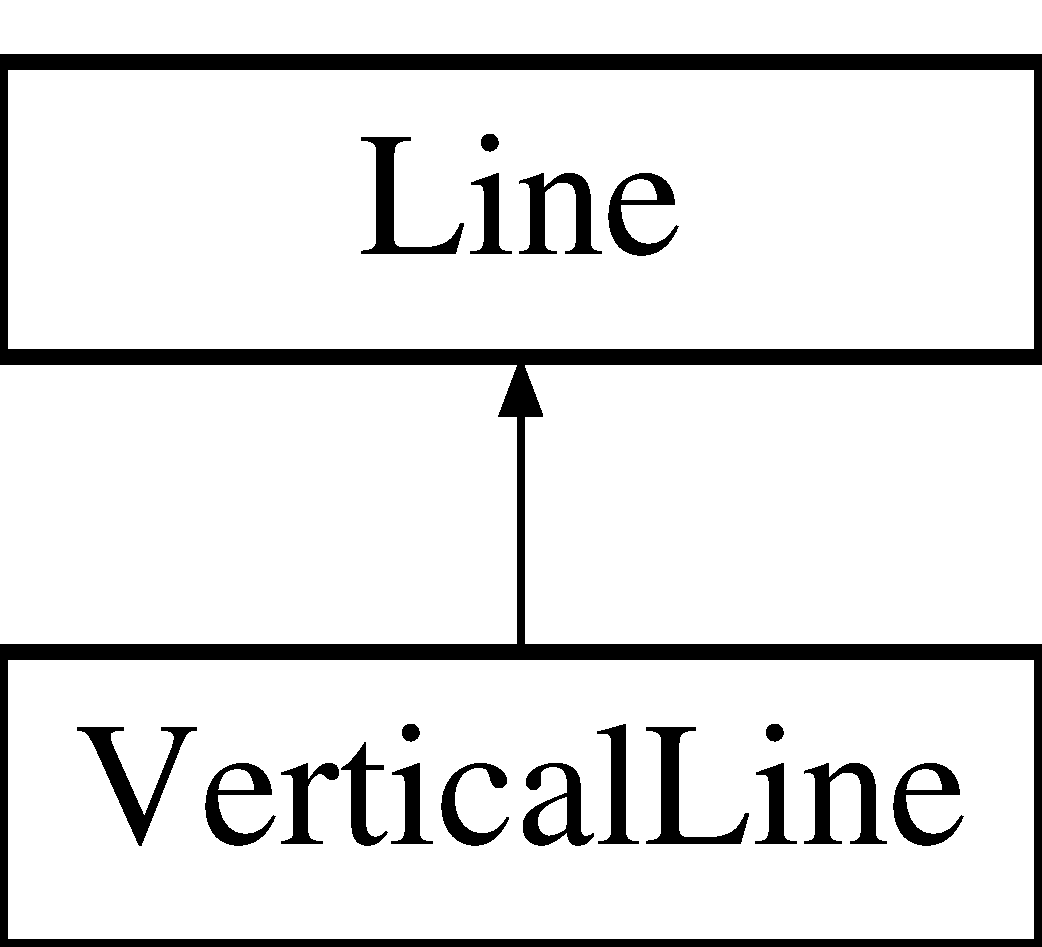
\includegraphics[height=2.000000cm]{classVerticalLine}
\end{center}
\end{figure}
\subsection*{\-Public \-Member \-Functions}
\begin{DoxyCompactItemize}
\item 
\hyperlink{classVerticalLine_a53b358b7ed8d9bbbaf7ee8b75e9a8665}{\-Vertical\-Line} (\hyperlink{classBox}{\-Box} $\ast$left, \hyperlink{classBox}{\-Box} $\ast$right, \-Q\-Object $\ast$parent=0)
\begin{DoxyCompactList}\small\item\em \-Default constructor. \end{DoxyCompactList}\item 
virtual \hyperlink{classVerticalLine_a925318f98ded156abcde65ccf60830d6}{$\sim$\-Vertical\-Line} ()
\begin{DoxyCompactList}\small\item\em \-Destructor. \end{DoxyCompactList}\item 
void \hyperlink{classVerticalLine_ae4ac7f318bec7b2ed7a90c1c31a3752d}{turn\-Grey} ()
\begin{DoxyCompactList}\small\item\em \-Makes the line grey. \end{DoxyCompactList}\item 
bool \hyperlink{classVerticalLine_ac90ef61324404c12668c73dc5567dc11}{play\-Turn} (bool user\-Turn)
\begin{DoxyCompactList}\small\item\em \-Called when a line is selected. \end{DoxyCompactList}\item 
\hyperlink{classBox}{\-Box} $\ast$ \hyperlink{classVerticalLine_a51e7a4f8a9f201ff3d4215373c1f9909}{get\-Left} () const 
\begin{DoxyCompactList}\small\item\em \-Gets the box to the left of the line. \end{DoxyCompactList}\item 
\hyperlink{classBox}{\-Box} $\ast$ \hyperlink{classVerticalLine_a6a7688ae8c09aca10a841874d8e835ea}{get\-Right} () const 
\begin{DoxyCompactList}\small\item\em \-Gets the box to the right of the line. \end{DoxyCompactList}\end{DoxyCompactItemize}


\subsection{\-Constructor \& \-Destructor \-Documentation}
\hypertarget{classVerticalLine_a53b358b7ed8d9bbbaf7ee8b75e9a8665}{\index{\-Vertical\-Line@{\-Vertical\-Line}!\-Vertical\-Line@{\-Vertical\-Line}}
\index{\-Vertical\-Line@{\-Vertical\-Line}!VerticalLine@{\-Vertical\-Line}}
\subsubsection[{\-Vertical\-Line}]{\setlength{\rightskip}{0pt plus 5cm}{\bf \-Vertical\-Line\-::\-Vertical\-Line} (
\begin{DoxyParamCaption}
\item[{{\bf \-Box} $\ast$}]{left, }
\item[{{\bf \-Box} $\ast$}]{right, }
\item[{\-Q\-Object $\ast$}]{parent = {\ttfamily 0}}
\end{DoxyParamCaption}
)\hspace{0.3cm}{\ttfamily  \mbox{[}explicit\mbox{]}}}}\label{classVerticalLine_a53b358b7ed8d9bbbaf7ee8b75e9a8665}


\-Default constructor. 


\begin{DoxyParams}{\-Parameters}
{\em left} & \hyperlink{classBox}{\-Box} on left of line \\
\hline
{\em right} & \hyperlink{classBox}{\-Box} on right of line\\
\hline
\end{DoxyParams}
\-Sets \hyperlink{classVerticalLine}{\-Vertical\-Line} properties. \hypertarget{classVerticalLine_a925318f98ded156abcde65ccf60830d6}{\index{\-Vertical\-Line@{\-Vertical\-Line}!$\sim$\-Vertical\-Line@{$\sim$\-Vertical\-Line}}
\index{$\sim$\-Vertical\-Line@{$\sim$\-Vertical\-Line}!VerticalLine@{\-Vertical\-Line}}
\subsubsection[{$\sim$\-Vertical\-Line}]{\setlength{\rightskip}{0pt plus 5cm}{\bf \-Vertical\-Line\-::$\sim$\-Vertical\-Line} (
\begin{DoxyParamCaption}
{}
\end{DoxyParamCaption}
)\hspace{0.3cm}{\ttfamily  \mbox{[}virtual\mbox{]}}}}\label{classVerticalLine_a925318f98ded156abcde65ccf60830d6}


\-Destructor. 

\-Frees allocated memory. 

\subsection{\-Member \-Function \-Documentation}
\hypertarget{classVerticalLine_a51e7a4f8a9f201ff3d4215373c1f9909}{\index{\-Vertical\-Line@{\-Vertical\-Line}!get\-Left@{get\-Left}}
\index{get\-Left@{get\-Left}!VerticalLine@{\-Vertical\-Line}}
\subsubsection[{get\-Left}]{\setlength{\rightskip}{0pt plus 5cm}{\bf \-Box} $\ast$ {\bf \-Vertical\-Line\-::get\-Left} (
\begin{DoxyParamCaption}
{}
\end{DoxyParamCaption}
) const}}\label{classVerticalLine_a51e7a4f8a9f201ff3d4215373c1f9909}


\-Gets the box to the left of the line. 

\begin{DoxyReturn}{\-Returns}
box to the left of the line
\end{DoxyReturn}
\-Returns the box to the left of the line. \hypertarget{classVerticalLine_a6a7688ae8c09aca10a841874d8e835ea}{\index{\-Vertical\-Line@{\-Vertical\-Line}!get\-Right@{get\-Right}}
\index{get\-Right@{get\-Right}!VerticalLine@{\-Vertical\-Line}}
\subsubsection[{get\-Right}]{\setlength{\rightskip}{0pt plus 5cm}{\bf \-Box} $\ast$ {\bf \-Vertical\-Line\-::get\-Right} (
\begin{DoxyParamCaption}
{}
\end{DoxyParamCaption}
) const}}\label{classVerticalLine_a6a7688ae8c09aca10a841874d8e835ea}


\-Gets the box to the right of the line. 

\begin{DoxyReturn}{\-Returns}
box to the right of the line
\end{DoxyReturn}
\-Returns the box to the right of the line. \hypertarget{classVerticalLine_ac90ef61324404c12668c73dc5567dc11}{\index{\-Vertical\-Line@{\-Vertical\-Line}!play\-Turn@{play\-Turn}}
\index{play\-Turn@{play\-Turn}!VerticalLine@{\-Vertical\-Line}}
\subsubsection[{play\-Turn}]{\setlength{\rightskip}{0pt plus 5cm}bool {\bf \-Vertical\-Line\-::play\-Turn} (
\begin{DoxyParamCaption}
\item[{bool}]{user\-Turn}
\end{DoxyParamCaption}
)\hspace{0.3cm}{\ttfamily  \mbox{[}virtual\mbox{]}}}}\label{classVerticalLine_ac90ef61324404c12668c73dc5567dc11}


\-Called when a line is selected. 


\begin{DoxyParams}{\-Parameters}
{\em user\-Turn} & \-Whether it is the user's turn \\
\hline
\end{DoxyParams}
\begin{DoxyReturn}{\-Returns}
\-Whether it is still the player's turn
\end{DoxyReturn}
\-Called when a line is drawn. \-Returns whether it is still the same player's turn. 

\-Implements \hyperlink{classLine_adb2af7d5815c082d2c7864a86af27b14}{\-Line}.

\hypertarget{classVerticalLine_ae4ac7f318bec7b2ed7a90c1c31a3752d}{\index{\-Vertical\-Line@{\-Vertical\-Line}!turn\-Grey@{turn\-Grey}}
\index{turn\-Grey@{turn\-Grey}!VerticalLine@{\-Vertical\-Line}}
\subsubsection[{turn\-Grey}]{\setlength{\rightskip}{0pt plus 5cm}void {\bf \-Vertical\-Line\-::turn\-Grey} (
\begin{DoxyParamCaption}
{}
\end{DoxyParamCaption}
)\hspace{0.3cm}{\ttfamily  \mbox{[}virtual\mbox{]}}}}\label{classVerticalLine_ae4ac7f318bec7b2ed7a90c1c31a3752d}


\-Makes the line grey. 

\-Changes the object image to make it grey. 

\-Implements \hyperlink{classLine_a63f54b0b50d2c6db91fc7d97c15433b1}{\-Line}.



\-The documentation for this class was generated from the following files\-:\begin{DoxyCompactItemize}
\item 
game3/\hyperlink{verticalline_8h}{verticalline.\-h}\item 
game3/\hyperlink{verticalline_8cpp}{verticalline.\-cpp}\end{DoxyCompactItemize}

\chapter{\-File \-Documentation}
\hypertarget{difficulty_8h}{\section{difficulty.\-h \-File \-Reference}
\label{difficulty_8h}\index{difficulty.\-h@{difficulty.\-h}}
}


\-Difficulty enum.  


\subsection*{\-Enumerations}
\begin{DoxyCompactItemize}
\item 
enum {\bfseries \-Difficulty} \{ \*
{\bfseries \-N\-O\-\_\-\-D\-I\-F\-F\-I\-C\-U\-L\-T\-Y}, 
{\bfseries \-E\-A\-S\-Y}, 
{\bfseries \-M\-O\-D\-E\-R\-A\-T\-E}, 
{\bfseries \-H\-A\-R\-D}, 
\*
{\bfseries \-D\-I\-F\-F\-I\-C\-U\-L\-T\-Y\-\_\-\-E\-N\-D}
 \}
\end{DoxyCompactItemize}


\subsection{\-Detailed \-Description}
\-Difficulty enum. \-This enum lists the different possible difficulties for games 2 and 3. \begin{DoxyAuthor}{\-Author}
\-Rita \-Aoun 

\-Rawan \-Moukalled 
\end{DoxyAuthor}

\hypertarget{barn_8cpp}{\section{game1/barn.cpp \-File \-Reference}
\label{barn_8cpp}\index{game1/barn.\-cpp@{game1/barn.\-cpp}}
}


\-Contains \hyperlink{classBarn}{\-Barn} class definition.  


{\ttfamily \#include \char`\"{}barn.\-h\char`\"{}}\*
{\ttfamily \#include \char`\"{}game1scene.\-h\char`\"{}}\*
{\ttfamily \#include $<$\-Q\-List$>$}\*


\subsection{\-Detailed \-Description}
\-Contains \hyperlink{classBarn}{\-Barn} class definition. 
\hypertarget{barn_8h}{\section{game1/barn.h \-File \-Reference}
\label{barn_8h}\index{game1/barn.\-h@{game1/barn.\-h}}
}


\hyperlink{classBarn}{\-Barn} class.  


{\ttfamily \#include $<$\-Qt\-Gui$>$}\*
{\ttfamily \#include $<$\-Q\-Timer$>$}\*
\subsection*{\-Classes}
\begin{DoxyCompactItemize}
\item 
class \hyperlink{classBarn}{\-Barn}
\end{DoxyCompactItemize}


\subsection{\-Detailed \-Description}
\hyperlink{classBarn}{\-Barn} class. \hyperlink{classBarn}{\-Barn} that terminates the game once a sheep from the line reaches it \begin{DoxyAuthor}{\-Author}
\-Rita \-Aoun 

\-Rawan \-Moukalled 
\end{DoxyAuthor}

\hypertarget{cannon_8cpp}{\section{game1/cannon.cpp \-File \-Reference}
\label{cannon_8cpp}\index{game1/cannon.\-cpp@{game1/cannon.\-cpp}}
}


\-Contains \hyperlink{classCannon}{\-Cannon} class definition.  


{\ttfamily \#include \char`\"{}cannon.\-h\char`\"{}}\*
{\ttfamily \#include \char`\"{}game1scene.\-h\char`\"{}}\*


\subsection{\-Detailed \-Description}
\-Contains \hyperlink{classCannon}{\-Cannon} class definition. 
\hypertarget{cannon_8h}{\section{game1/cannon.h \-File \-Reference}
\label{cannon_8h}\index{game1/cannon.\-h@{game1/cannon.\-h}}
}


\hyperlink{classCannon}{\-Cannon} class.  


{\ttfamily \#include $<$\-Qt\-Gui$>$}\*
\subsection*{\-Classes}
\begin{DoxyCompactItemize}
\item 
class \hyperlink{classCannon}{\-Cannon}
\end{DoxyCompactItemize}


\subsection{\-Detailed \-Description}
\hyperlink{classCannon}{\-Cannon} class. \hyperlink{classCannon}{\-Cannon} objects rotate with mouse movements, and fire sheep on click. \begin{DoxyAuthor}{\-Author}
\-Rita \-Aoun 

\-Rawan \-Moukalled 
\end{DoxyAuthor}

\hypertarget{game1_8cpp}{\section{game1.\-cpp \-File \-Reference}
\label{game1_8cpp}\index{game1.\-cpp@{game1.\-cpp}}
}


\-Contains the \-Sheep \-Line.  


{\ttfamily \#include \char`\"{}game1.\-h\char`\"{}}\*
{\ttfamily \#include \char`\"{}helper.\-h\char`\"{}}\*
{\ttfamily \#include \char`\"{}gamemainmenu.\-h\char`\"{}}\*


\subsection{\-Detailed \-Description}
\-Contains the \-Sheep \-Line. 
\hypertarget{game1_8h}{\section{game1.\-h \-File \-Reference}
\label{game1_8h}\index{game1.\-h@{game1.\-h}}
}


\-Sheep \-Line class.  


{\ttfamily \#include $<$\-Q\-Widget$>$}\*
{\ttfamily \#include $<$\-Qt\-Gui$>$}\*
\subsection*{\-Classes}
\begin{DoxyCompactItemize}
\item 
class \hyperlink{classGame1}{\-Game1}
\end{DoxyCompactItemize}


\subsection{\-Detailed \-Description}
\-Sheep \-Line class. \-This is the class for the gameplay of the \-Sheep \-Line game. \begin{DoxyAuthor}{\-Author}
\-Rita \-Aoun 

\-Rawan \-Moukalled 
\end{DoxyAuthor}

\hypertarget{game1options_8cpp}{\section{game1/game1options.cpp \-File \-Reference}
\label{game1options_8cpp}\index{game1/game1options.\-cpp@{game1/game1options.\-cpp}}
}


\-Contains \hyperlink{classGame1Options}{\-Game1\-Options} class definition.  


{\ttfamily \#include \char`\"{}game1/game1options.\-h\char`\"{}}\*
{\ttfamily \#include \char`\"{}helper.\-h\char`\"{}}\*
{\ttfamily \#include \char`\"{}gui/gamemainmenu.\-h\char`\"{}}\*
{\ttfamily \#include \char`\"{}game1/game1.\-h\char`\"{}}\*
{\ttfamily \#include $<$\-Q\-Sql\-Query$>$}\*


\subsection{\-Detailed \-Description}
\-Contains \hyperlink{classGame1Options}{\-Game1\-Options} class definition. 
\hypertarget{game1options_8h}{\section{game1/game1options.h \-File \-Reference}
\label{game1options_8h}\index{game1/game1options.\-h@{game1/game1options.\-h}}
}


\hyperlink{classGame1Options}{\-Game1\-Options} class.  


{\ttfamily \#include $<$\-Qt\-Gui$>$}\*
\subsection*{\-Classes}
\begin{DoxyCompactItemize}
\item 
class \hyperlink{classGame1Options}{\-Game1\-Options}
\end{DoxyCompactItemize}


\subsection{\-Detailed \-Description}
\hyperlink{classGame1Options}{\-Game1\-Options} class. \-This is the options page for game 1, where the user can choose the level with which to start the game. \-Only unlocked levels can be accessed. \begin{DoxyAuthor}{\-Author}
\-Rita \-Aoun 

\-Rawan \-Moukalled 
\end{DoxyAuthor}

\hypertarget{game1scene_8cpp}{\section{game1/game1scene.cpp \-File \-Reference}
\label{game1scene_8cpp}\index{game1/game1scene.\-cpp@{game1/game1scene.\-cpp}}
}


\-Contains \hyperlink{classGame1Scene}{\-Game1\-Scene} class definition.  


{\ttfamily \#include \char`\"{}game1scene.\-h\char`\"{}}\*
{\ttfamily \#include \char`\"{}helper.\-h\char`\"{}}\*
{\ttfamily \#include $<$\-Q\-Vector$>$}\*
{\ttfamily \#include $<$\-Q\-Set$>$}\*
{\ttfamily \#include \char`\"{}game1options.\-h\char`\"{}}\*


\subsection{\-Detailed \-Description}
\-Contains \hyperlink{classGame1Scene}{\-Game1\-Scene} class definition. 
\hypertarget{game1scene_8h}{\section{game1/game1scene.h \-File \-Reference}
\label{game1scene_8h}\index{game1/game1scene.\-h@{game1/game1scene.\-h}}
}


\-Sheep \-Line class.  


{\ttfamily \#include $<$\-Qt\-Gui$>$}\*
{\ttfamily \#include $<$\-Q\-Linked\-List$>$}\*
{\ttfamily \#include $<$\-Q\-Timer$>$}\*
{\ttfamily \#include \char`\"{}game1/cannon.\-h\char`\"{}}\*
{\ttfamily \#include \char`\"{}game1/sheep1.\-h\char`\"{}}\*
{\ttfamily \#include \char`\"{}game1/barn.\-h\char`\"{}}\*
{\ttfamily \#include \char`\"{}game1/gameover.\-h\char`\"{}}\*
\subsection*{\-Classes}
\begin{DoxyCompactItemize}
\item 
class \hyperlink{classGame1Scene}{\-Game1\-Scene}
\end{DoxyCompactItemize}


\subsection{\-Detailed \-Description}
\-Sheep \-Line class. \-Implements the scene of \-Game 1\-: \-Sheep \-Line \begin{DoxyAuthor}{\-Author}
\-Rita \-Aoun 

\-Rawan \-Moukalled 
\end{DoxyAuthor}

\hypertarget{sheep1_8cpp}{\section{game1/sheep1.cpp \-File \-Reference}
\label{sheep1_8cpp}\index{game1/sheep1.\-cpp@{game1/sheep1.\-cpp}}
}


\-Contains \hyperlink{classSheep1}{\-Sheep1} class definition.  


{\ttfamily \#include \char`\"{}sheep1.\-h\char`\"{}}\*
{\ttfamily \#include \char`\"{}helper.\-h\char`\"{}}\*
{\ttfamily \#include \char`\"{}game1scene.\-h\char`\"{}}\*
{\ttfamily \#include $<$\-Q\-String$>$}\*


\subsection{\-Detailed \-Description}
\-Contains \hyperlink{classSheep1}{\-Sheep1} class definition. 
\hypertarget{sheep1_8h}{\section{game1/sheep1.h \-File \-Reference}
\label{sheep1_8h}\index{game1/sheep1.\-h@{game1/sheep1.\-h}}
}


\hyperlink{classSheep1}{\-Sheep1} class.  


{\ttfamily \#include $<$\-Qt\-Gui$>$}\*
{\ttfamily \#include $<$\-Q\-Timer$>$}\*
\subsection*{\-Classes}
\begin{DoxyCompactItemize}
\item 
class \hyperlink{classSheep1}{\-Sheep1}
\end{DoxyCompactItemize}


\subsection{\-Detailed \-Description}
\hyperlink{classSheep1}{\-Sheep1} class. \-Randomly numbered sheep that are used for \-Game 1\-: \-Sheep \hyperlink{classLine}{\-Line} \begin{DoxyAuthor}{\-Author}
\-Rita \-Aoun 

\-Rawan \-Moukalled 
\end{DoxyAuthor}

\hypertarget{game2_8cpp}{\section{game2.\-cpp \-File \-Reference}
\label{game2_8cpp}\index{game2.\-cpp@{game2.\-cpp}}
}


\-Contains the \-Trap the \-Sheep game.  


{\ttfamily \#include \char`\"{}game2.\-h\char`\"{}}\*
{\ttfamily \#include \char`\"{}helper.\-h\char`\"{}}\*
{\ttfamily \#include \char`\"{}gamemainmenu.\-h\char`\"{}}\*


\subsection{\-Detailed \-Description}
\-Contains the \-Trap the \-Sheep game. 
\hypertarget{game2_8h}{\section{game2/game2.h \-File \-Reference}
\label{game2_8h}\index{game2/game2.\-h@{game2/game2.\-h}}
}


\-Trap the \-Sheep class.  


{\ttfamily \#include $<$\-Qt\-Gui$>$}\*
\subsection*{\-Classes}
\begin{DoxyCompactItemize}
\item 
class \hyperlink{classGame2}{\-Game2}
\end{DoxyCompactItemize}


\subsection{\-Detailed \-Description}
\-Trap the \-Sheep class. \-This is the class for the gameplay of the \-Trap the \-Sheep game. \begin{DoxyAuthor}{\-Author}
\-Rita \-Aoun 

\-Rawan \-Moukalled 
\end{DoxyAuthor}

\hypertarget{game2options_8cpp}{\section{game2/game2options.cpp \-File \-Reference}
\label{game2options_8cpp}\index{game2/game2options.\-cpp@{game2/game2options.\-cpp}}
}


\-Contains \hyperlink{classGame2Options}{\-Game2\-Options} class definition.  


{\ttfamily \#include \char`\"{}game2/game2options.\-h\char`\"{}}\*
{\ttfamily \#include \char`\"{}helper.\-h\char`\"{}}\*
{\ttfamily \#include \char`\"{}game2/game2.\-h\char`\"{}}\*
{\ttfamily \#include \char`\"{}gui/gamemainmenu.\-h\char`\"{}}\*


\subsection{\-Detailed \-Description}
\-Contains \hyperlink{classGame2Options}{\-Game2\-Options} class definition. 
\hypertarget{game2options_8h}{\section{game2/game2options.h \-File \-Reference}
\label{game2options_8h}\index{game2/game2options.\-h@{game2/game2options.\-h}}
}


\hyperlink{classGame2Options}{\-Game2\-Options} class.  


{\ttfamily \#include $<$\-Qt\-Gui$>$}\*
{\ttfamily \#include \char`\"{}difficulty.\-h\char`\"{}}\*
\subsection*{\-Classes}
\begin{DoxyCompactItemize}
\item 
class \hyperlink{classGame2Options}{\-Game2\-Options}
\end{DoxyCompactItemize}


\subsection{\-Detailed \-Description}
\hyperlink{classGame2Options}{\-Game2\-Options} class. \-This is the options page for game 2, where the user can choose the level with which to start the game. \-Levels are\-: \-Easy, \-Moderate and \-Hard. \begin{DoxyAuthor}{\-Author}
\-Rita \-Aoun 

\-Rawan \-Moukalled 
\end{DoxyAuthor}

\hypertarget{game2scene_8cpp}{\section{game2/game2scene.cpp \-File \-Reference}
\label{game2scene_8cpp}\index{game2/game2scene.\-cpp@{game2/game2scene.\-cpp}}
}


\-Contains \hyperlink{classGame2Scene}{\-Game2\-Scene} class definition.  


{\ttfamily \#include \char`\"{}game2scene.\-h\char`\"{}}\*
{\ttfamily \#include $<$climits$>$}\*
{\ttfamily \#include $<$\-Q\-Sql\-Query$>$}\*
{\ttfamily \#include \char`\"{}helper.\-h\char`\"{}}\*


\subsection{\-Detailed \-Description}
\-Contains \hyperlink{classGame2Scene}{\-Game2\-Scene} class definition. 
\hypertarget{game2scene_8h}{\section{game2/game2scene.h \-File \-Reference}
\label{game2scene_8h}\index{game2/game2scene.\-h@{game2/game2scene.\-h}}
}


\-Trap the \-Sheep scene class.  


{\ttfamily \#include $<$\-Q\-Graphics\-Scene$>$}\*
{\ttfamily \#include $<$\-Qt\-Gui$>$}\*
{\ttfamily \#include \char`\"{}difficulty.\-h\char`\"{}}\*
{\ttfamily \#include \char`\"{}game2/tile.\-h\char`\"{}}\*
{\ttfamily \#include \char`\"{}game2/sheep2.\-h\char`\"{}}\*
{\ttfamily \#include \char`\"{}gameover.\-h\char`\"{}}\*
\subsection*{\-Classes}
\begin{DoxyCompactItemize}
\item 
class \hyperlink{classGame2Scene}{\-Game2\-Scene}
\end{DoxyCompactItemize}


\subsection{\-Detailed \-Description}
\-Trap the \-Sheep scene class. \-This is the scene class for the gameplay of the \-Trap the \-Sheep game. \begin{DoxyAuthor}{\-Author}
\-Rita \-Aoun 

\-Rawan \-Moukalled 
\end{DoxyAuthor}

\hypertarget{sheep2_8cpp}{\section{game2/sheep2.cpp \-File \-Reference}
\label{sheep2_8cpp}\index{game2/sheep2.\-cpp@{game2/sheep2.\-cpp}}
}


\-Contains \-Sheep class definition.  


{\ttfamily \#include \char`\"{}sheep2.\-h\char`\"{}}\*


\subsection{\-Detailed \-Description}
\-Contains \-Sheep class definition. 
\hypertarget{tile_8cpp}{\section{game2/tile.cpp \-File \-Reference}
\label{tile_8cpp}\index{game2/tile.\-cpp@{game2/tile.\-cpp}}
}


\-Contains \hyperlink{classTile}{\-Tile} class definition.  


{\ttfamily \#include \char`\"{}tile.\-h\char`\"{}}\*
{\ttfamily \#include \char`\"{}game2scene.\-h\char`\"{}}\*
{\ttfamily \#include \char`\"{}sheep2.\-h\char`\"{}}\*


\subsection{\-Detailed \-Description}
\-Contains \hyperlink{classTile}{\-Tile} class definition. 
\hypertarget{tile_8h}{\section{game2/tile.h \-File \-Reference}
\label{tile_8h}\index{game2/tile.\-h@{game2/tile.\-h}}
}


class for the tiles of game 2  


{\ttfamily \#include $<$\-Qt\-Gui$>$}\*
{\ttfamily \#include $<$\-Q\-Mouse\-Event$>$}\*
\subsection*{\-Classes}
\begin{DoxyCompactItemize}
\item 
class \hyperlink{classTile}{\-Tile}
\end{DoxyCompactItemize}


\subsection{\-Detailed \-Description}
class for the tiles of game 2 \-This is class for the tiles of the grid in game 2 \begin{DoxyAuthor}{\-Author}
\-Rita \-Aoun 

\-Rawan \-Moukalled 
\end{DoxyAuthor}

\hypertarget{box_8cpp}{\section{game3/box.cpp \-File \-Reference}
\label{box_8cpp}\index{game3/box.\-cpp@{game3/box.\-cpp}}
}


\-Contains \hyperlink{classBox}{\-Box} class definition.  


{\ttfamily \#include \char`\"{}box.\-h\char`\"{}}\*


\subsection{\-Detailed \-Description}
\-Contains \hyperlink{classBox}{\-Box} class definition. 
\hypertarget{box_8h}{\section{game3/box.h \-File \-Reference}
\label{box_8h}\index{game3/box.\-h@{game3/box.\-h}}
}


\hyperlink{classBox}{\-Box} class.  


{\ttfamily \#include $<$\-Qt\-Gui$>$}\*
\subsection*{\-Classes}
\begin{DoxyCompactItemize}
\item 
class \hyperlink{classBox}{\-Box}
\end{DoxyCompactItemize}


\subsection{\-Detailed \-Description}
\hyperlink{classBox}{\-Box} class. \hyperlink{classBox}{\-Box} objects need to be bounded by a player for them to win points. \begin{DoxyAuthor}{\-Author}
\-Rita \-Aoun 

\-Rawan \-Moukalled 
\end{DoxyAuthor}

\hypertarget{dot_8cpp}{\section{game3/dot.cpp \-File \-Reference}
\label{dot_8cpp}\index{game3/dot.\-cpp@{game3/dot.\-cpp}}
}


\-Contains \hyperlink{classDot}{\-Dot} class definition.  


{\ttfamily \#include \char`\"{}dot.\-h\char`\"{}}\*


\subsection{\-Detailed \-Description}
\-Contains \hyperlink{classDot}{\-Dot} class definition. 
\hypertarget{dot_8h}{\section{game3/dot.h \-File \-Reference}
\label{dot_8h}\index{game3/dot.\-h@{game3/dot.\-h}}
}


\hyperlink{classDot}{\-Dot} class.  


{\ttfamily \#include $<$\-Qt\-Gui$>$}\*
\subsection*{\-Classes}
\begin{DoxyCompactItemize}
\item 
class \hyperlink{classDot}{\-Dot}
\end{DoxyCompactItemize}


\subsection{\-Detailed \-Description}
\hyperlink{classDot}{\-Dot} class. \hyperlink{classDot}{\-Dot} objects delimit the game lines. \begin{DoxyAuthor}{\-Author}
\-Rita \-Aoun 

\-Rawan \-Moukalled 
\end{DoxyAuthor}

\hypertarget{game3_8cpp}{\section{game3/game3.cpp \-File \-Reference}
\label{game3_8cpp}\index{game3/game3.\-cpp@{game3/game3.\-cpp}}
}


\-Contains the \-Dots and \-Lines game.  


{\ttfamily \#include \char`\"{}game3/game3.\-h\char`\"{}}\*
{\ttfamily \#include \char`\"{}helper.\-h\char`\"{}}\*
{\ttfamily \#include \char`\"{}gui/gamemainmenu.\-h\char`\"{}}\*
{\ttfamily \#include $<$\-Q\-Sql\-Query$>$}\*


\subsection{\-Detailed \-Description}
\-Contains the \-Dots and \-Lines game. 
\hypertarget{game3_8h}{\section{game3/game3.h \-File \-Reference}
\label{game3_8h}\index{game3/game3.\-h@{game3/game3.\-h}}
}


\-Dots and \-Lines class.  


{\ttfamily \#include $<$\-Qt\-Gui$>$}\*
\subsection*{\-Classes}
\begin{DoxyCompactItemize}
\item 
class \hyperlink{classGame3}{\-Game3}
\end{DoxyCompactItemize}


\subsection{\-Detailed \-Description}
\-Dots and \-Lines class. \-This is the class for the gameplay of the \-Dots and \-Lines game. \begin{DoxyAuthor}{\-Author}
\-Rita \-Aoun 

\-Rawan \-Moukalled 
\end{DoxyAuthor}

\hypertarget{game3options_8cpp}{\section{game3/game3options.cpp \-File \-Reference}
\label{game3options_8cpp}\index{game3/game3options.\-cpp@{game3/game3options.\-cpp}}
}


\-Contains \hyperlink{classGame3Options}{\-Game3\-Options} class definition.  


{\ttfamily \#include \char`\"{}game3options.\-h\char`\"{}}\*
{\ttfamily \#include \char`\"{}helper.\-h\char`\"{}}\*
{\ttfamily \#include \char`\"{}game3/game3.\-h\char`\"{}}\*
{\ttfamily \#include \char`\"{}gui/gamemainmenu.\-h\char`\"{}}\*


\subsection{\-Detailed \-Description}
\-Contains \hyperlink{classGame3Options}{\-Game3\-Options} class definition. 
\hypertarget{game3options_8h}{\section{game3/game3options.h \-File \-Reference}
\label{game3options_8h}\index{game3/game3options.\-h@{game3/game3options.\-h}}
}


\hyperlink{classGame3Options}{\-Game3\-Options} class.  


{\ttfamily \#include $<$\-Qt\-Gui$>$}\*
{\ttfamily \#include \char`\"{}difficulty.\-h\char`\"{}}\*
{\ttfamily \#include \char`\"{}game3/size.\-h\char`\"{}}\*
\subsection*{\-Classes}
\begin{DoxyCompactItemize}
\item 
class \hyperlink{classGame3Options}{\-Game3\-Options}
\end{DoxyCompactItemize}


\subsection{\-Detailed \-Description}
\hyperlink{classGame3Options}{\-Game3\-Options} class. \-This is the options page for game 3, where the user can choose the level and size with which to start the game. \-Levels are\-: \-Easy, \-Moderate and \-Hard. \-Sizes are\-: 4x4, 8x8, 16x16.

\begin{DoxyAuthor}{\-Author}
\-Rita \-Aoun 

\-Rawan \-Moukalled 
\end{DoxyAuthor}

\hypertarget{game3scene_8cpp}{\section{game3/game3scene.cpp \-File \-Reference}
\label{game3scene_8cpp}\index{game3/game3scene.\-cpp@{game3/game3scene.\-cpp}}
}


\-Contains \hyperlink{classGame3Scene}{\-Game3\-Scene} class definition.  


{\ttfamily \#include \char`\"{}game3scene.\-h\char`\"{}}\*


\subsection{\-Detailed \-Description}
\-Contains \hyperlink{classGame3Scene}{\-Game3\-Scene} class definition. 
\hypertarget{game3scene_8h}{\section{game3/game3scene.h \-File \-Reference}
\label{game3scene_8h}\index{game3/game3scene.\-h@{game3/game3scene.\-h}}
}


\hyperlink{classGame3Scene}{\-Game3\-Scene} class.  


{\ttfamily \#include $<$\-Qt\-Gui$>$}\*
{\ttfamily \#include \char`\"{}difficulty.\-h\char`\"{}}\*
{\ttfamily \#include \char`\"{}game3/size.\-h\char`\"{}}\*
{\ttfamily \#include \char`\"{}game3/dot.\-h\char`\"{}}\*
{\ttfamily \#include \char`\"{}game3/horizontalline.\-h\char`\"{}}\*
{\ttfamily \#include \char`\"{}game3/verticalline.\-h\char`\"{}}\*
{\ttfamily \#include \char`\"{}gameover.\-h\char`\"{}}\*
\subsection*{\-Classes}
\begin{DoxyCompactItemize}
\item 
class \hyperlink{classGame3Scene}{\-Game3\-Scene}
\end{DoxyCompactItemize}


\subsection{\-Detailed \-Description}
\hyperlink{classGame3Scene}{\-Game3\-Scene} class. \-This is the scene for game 3, \-Dots and \-Lines.

\begin{DoxyAuthor}{\-Author}
\-Rita \-Aoun 

\-Rawan \-Moukalled 
\end{DoxyAuthor}

\hypertarget{horizontalline_8cpp}{\section{game3/horizontalline.cpp \-File \-Reference}
\label{horizontalline_8cpp}\index{game3/horizontalline.\-cpp@{game3/horizontalline.\-cpp}}
}


\-Contains \hyperlink{classHorizontalLine}{\-Horizontal\-Line} class definition.  


{\ttfamily \#include \char`\"{}horizontalline.\-h\char`\"{}}\*
{\ttfamily \#include \char`\"{}game3/game3scene.\-h\char`\"{}}\*


\subsection{\-Detailed \-Description}
\-Contains \hyperlink{classHorizontalLine}{\-Horizontal\-Line} class definition. 
\hypertarget{horizontalline_8h}{\section{game3/horizontalline.h \-File \-Reference}
\label{horizontalline_8h}\index{game3/horizontalline.\-h@{game3/horizontalline.\-h}}
}


\hyperlink{classHorizontalLine}{\-Horizontal\-Line} class.  


{\ttfamily \#include \char`\"{}game3/line.\-h\char`\"{}}\*
{\ttfamily \#include \char`\"{}game3/box.\-h\char`\"{}}\*
\subsection*{\-Classes}
\begin{DoxyCompactItemize}
\item 
class \hyperlink{classHorizontalLine}{\-Horizontal\-Line}
\end{DoxyCompactItemize}


\subsection{\-Detailed \-Description}
\hyperlink{classHorizontalLine}{\-Horizontal\-Line} class. \-Horizontal lines that delimit boxes from the top and bottom. \begin{DoxyAuthor}{\-Author}
\-Rita \-Aoun 

\-Rawan \-Moukalled 
\end{DoxyAuthor}

\hypertarget{line_8cpp}{\section{game3/line.cpp \-File \-Reference}
\label{line_8cpp}\index{game3/line.\-cpp@{game3/line.\-cpp}}
}


\-Contains \hyperlink{classLine}{\-Line} class definition.  


{\ttfamily \#include \char`\"{}line.\-h\char`\"{}}\*
{\ttfamily \#include \char`\"{}game3/game3scene.\-h\char`\"{}}\*


\subsection{\-Detailed \-Description}
\-Contains \hyperlink{classLine}{\-Line} class definition. 
\hypertarget{line_8h}{\section{game3/line.h \-File \-Reference}
\label{line_8h}\index{game3/line.\-h@{game3/line.\-h}}
}


\hyperlink{classLine}{\-Line} class.  


{\ttfamily \#include $<$\-Qt\-Gui$>$}\*
\subsection*{\-Classes}
\begin{DoxyCompactItemize}
\item 
class \hyperlink{classLine}{\-Line}
\end{DoxyCompactItemize}


\subsection{\-Detailed \-Description}
\hyperlink{classLine}{\-Line} class. \hyperlink{classLine}{\-Line} is an interface for vertical and horizontal lines. \-It implements the on-\/click reaction of lines and it remembers whether a line has been clicked before.

\begin{DoxyAuthor}{\-Author}
\-Rita \-Aoun 

\-Rawan \-Moukalled 
\end{DoxyAuthor}

\hypertarget{size_8h}{\section{game3/size.h \-File \-Reference}
\label{size_8h}\index{game3/size.\-h@{game3/size.\-h}}
}


\-Size enum.  


\subsection*{\-Enumerations}
\begin{DoxyCompactItemize}
\item 
enum {\bfseries \-Size} \{ \*
{\bfseries \-N\-O\-\_\-\-S\-I\-Z\-E}, 
{\bfseries \-F\-O\-U\-R\-B\-Y\-F\-O\-U\-R} = 4, 
{\bfseries \-E\-I\-G\-H\-T\-B\-Y\-E\-I\-G\-H\-T} = 8, 
{\bfseries \-S\-I\-X\-T\-E\-E\-N\-B\-Y\-S\-I\-X\-T\-E\-E\-N} = 16, 
\*
{\bfseries \-S\-I\-Z\-E\-\_\-\-E\-N\-D}
 \}
\end{DoxyCompactItemize}


\subsection{\-Detailed \-Description}
\-Size enum. \-This enum lists the different possible sizes of the game 3 grid. \begin{DoxyAuthor}{\-Author}
\-Rita \-Aoun 

\-Rawan \-Moukalled 
\end{DoxyAuthor}

\hypertarget{verticalline_8cpp}{\section{game3/verticalline.cpp \-File \-Reference}
\label{verticalline_8cpp}\index{game3/verticalline.\-cpp@{game3/verticalline.\-cpp}}
}


\-Contains \hyperlink{classVerticalLine}{\-Vertical\-Line} class definition.  


{\ttfamily \#include \char`\"{}verticalline.\-h\char`\"{}}\*
{\ttfamily \#include \char`\"{}game3/game3scene.\-h\char`\"{}}\*


\subsection{\-Detailed \-Description}
\-Contains \hyperlink{classVerticalLine}{\-Vertical\-Line} class definition. 
\hypertarget{verticalline_8h}{\section{game3/verticalline.h \-File \-Reference}
\label{verticalline_8h}\index{game3/verticalline.\-h@{game3/verticalline.\-h}}
}


\hyperlink{classVerticalLine}{\-Vertical\-Line} class.  


{\ttfamily \#include $<$game3/line.\-h$>$}\*
{\ttfamily \#include \char`\"{}game3/box.\-h\char`\"{}}\*
\subsection*{\-Classes}
\begin{DoxyCompactItemize}
\item 
class \hyperlink{classVerticalLine}{\-Vertical\-Line}
\end{DoxyCompactItemize}


\subsection{\-Detailed \-Description}
\hyperlink{classVerticalLine}{\-Vertical\-Line} class. \-Vertical lines that delimit boxes from the left and right. \begin{DoxyAuthor}{\-Author}
\-Rita \-Aoun 

\-Rawan \-Moukalled 
\end{DoxyAuthor}

\hypertarget{gameover_8cpp}{\section{game1/gameover.cpp \-File \-Reference}
\label{gameover_8cpp}\index{game1/gameover.\-cpp@{game1/gameover.\-cpp}}
}


\-Contains \hyperlink{classGameOver}{\-Game\-Over} class definition.  


{\ttfamily \#include \char`\"{}gameover.\-h\char`\"{}}\*


\subsection{\-Detailed \-Description}
\-Contains \hyperlink{classGameOver}{\-Game\-Over} class definition. 
\hypertarget{gameover_8h}{\section{gameover.\-h \-File \-Reference}
\label{gameover_8h}\index{gameover.\-h@{gameover.\-h}}
}


\-Game \-Over class.  


{\ttfamily \#include $<$\-Qt\-Gui$>$}\*
\subsection*{\-Classes}
\begin{DoxyCompactItemize}
\item 
class \hyperlink{classGameOver}{\-Game\-Over}
\end{DoxyCompactItemize}


\subsection{\-Detailed \-Description}
\-Game \-Over class. \-Image overlayed on the screen when game is over \begin{DoxyAuthor}{\-Author}
\-Rita \-Aoun 

\-Rawan \-Moukalled 
\end{DoxyAuthor}

\hypertarget{gamemainmenu_8cpp}{\section{gui/gamemainmenu.cpp \-File \-Reference}
\label{gamemainmenu_8cpp}\index{gui/gamemainmenu.\-cpp@{gui/gamemainmenu.\-cpp}}
}


\-Contains \hyperlink{classGameMainMenu}{\-Game\-Main\-Menu} class definition.  


{\ttfamily \#include \char`\"{}gui/gamemainmenu.\-h\char`\"{}}\*
{\ttfamily \#include \char`\"{}helper.\-h\char`\"{}}\*
{\ttfamily \#include \char`\"{}game1/game1options.\-h\char`\"{}}\*
{\ttfamily \#include \char`\"{}games23options.\-h\char`\"{}}\*
{\ttfamily \#include \char`\"{}gui/gameselection.\-h\char`\"{}}\*


\subsection{\-Detailed \-Description}
\-Contains \hyperlink{classGameMainMenu}{\-Game\-Main\-Menu} class definition. 
\hypertarget{gamemainmenu_8h}{\section{gamemainmenu.\-h \-File \-Reference}
\label{gamemainmenu_8h}\index{gamemainmenu.\-h@{gamemainmenu.\-h}}
}


\hyperlink{classGameMainMenu}{\-Game\-Main\-Menu} class.  


{\ttfamily \#include $<$\-Q\-Widget$>$}\*
{\ttfamily \#include $<$\-Qt\-Gui$>$}\*
\subsection*{\-Classes}
\begin{DoxyCompactItemize}
\item 
class \hyperlink{classGameMainMenu}{\-Game\-Main\-Menu}
\end{DoxyCompactItemize}


\subsection{\-Detailed \-Description}
\hyperlink{classGameMainMenu}{\-Game\-Main\-Menu} class. \-This is the main game menu, where the user choose between resuming a previous game or starting a new one. \-The instructions are also shown on this menu. \begin{DoxyAuthor}{\-Author}
\-Rita \-Aoun 

\-Rawan \-Moukalled 
\end{DoxyAuthor}

\hypertarget{gameselection_8cpp}{\section{gameselection.\-cpp \-File \-Reference}
\label{gameselection_8cpp}\index{gameselection.\-cpp@{gameselection.\-cpp}}
}


\-Contains \hyperlink{classGameSelection}{\-Game\-Selection} class definition.  


{\ttfamily \#include \char`\"{}gameselection.\-h\char`\"{}}\*
{\ttfamily \#include \char`\"{}helper.\-h\char`\"{}}\*
{\ttfamily \#include \char`\"{}mainwidget.\-h\char`\"{}}\*
{\ttfamily \#include \char`\"{}gamemainmenu.\-h\char`\"{}}\*
{\ttfamily \#include \char`\"{}myaccount.\-h\char`\"{}}\*


\subsection{\-Detailed \-Description}
\-Contains \hyperlink{classGameSelection}{\-Game\-Selection} class definition. 
\hypertarget{gameselection_8h}{\section{gameselection.\-h \-File \-Reference}
\label{gameselection_8h}\index{gameselection.\-h@{gameselection.\-h}}
}


\-Game selection menu class.  


{\ttfamily \#include $<$\-Q\-Widget$>$}\*
{\ttfamily \#include $<$\-Qt\-Gui$>$}\*
{\ttfamily \#include $<$\-Q\-Application$>$}\*
{\ttfamily \#include $<$\-Q\-Graphics\-Scene$>$}\*
\subsection*{\-Classes}
\begin{DoxyCompactItemize}
\item 
class \hyperlink{classGameSelection}{\-Game\-Selection}
\end{DoxyCompactItemize}


\subsection{\-Detailed \-Description}
\-Game selection menu class. \-Game selection menu, where the user can select one of the three games available. \begin{DoxyAuthor}{\-Author}
\-Rita \-Aoun 

\-Rawan \-Moukalled 
\end{DoxyAuthor}

\hypertarget{mainwidget_8cpp}{\section{mainwidget.\-cpp \-File \-Reference}
\label{mainwidget_8cpp}\index{mainwidget.\-cpp@{mainwidget.\-cpp}}
}


\-Contains \hyperlink{classMainWidget}{\-Main\-Widget} class definition.  


{\ttfamily \#include \char`\"{}mainwidget.\-h\char`\"{}}\*
{\ttfamily \#include \char`\"{}gameselection.\-h\char`\"{}}\*


\subsection{\-Detailed \-Description}
\-Contains \hyperlink{classMainWidget}{\-Main\-Widget} class definition. 
\hypertarget{mainwidget_8h}{\section{mainwidget.\-h \-File \-Reference}
\label{mainwidget_8h}\index{mainwidget.\-h@{mainwidget.\-h}}
}


\hyperlink{classMainWidget}{\-Main\-Widget} class.  


{\ttfamily \#include $<$\-Q\-Widget$>$}\*
{\ttfamily \#include $<$\-Q\-Line\-Edit$>$}\*
{\ttfamily \#include $<$\-Q\-Label$>$}\*
{\ttfamily \#include $<$\-Q\-H\-Box\-Layout$>$}\*
{\ttfamily \#include $<$\-Q\-V\-Box\-Layout$>$}\*
{\ttfamily \#include $<$\-Q\-Grid\-Layout$>$}\*
{\ttfamily \#include $<$\-Q\-Push\-Button$>$}\*
\subsection*{\-Classes}
\begin{DoxyCompactItemize}
\item 
class \hyperlink{classMainWidget}{\-Main\-Widget}
\end{DoxyCompactItemize}


\subsection{\-Detailed \-Description}
\hyperlink{classMainWidget}{\-Main\-Widget} class. \-This is the main sign in window, where the user is given the chance to go on as a guest or to login/sign up. \begin{DoxyAuthor}{\-Author}
\-Rita \-Aoun 

\-Rawan \-Moukalled 
\end{DoxyAuthor}

\hypertarget{helper_8cpp}{\section{helper.\-cpp \-File \-Reference}
\label{helper_8cpp}\index{helper.\-cpp@{helper.\-cpp}}
}


\-Contains \hyperlink{classHelper}{\-Helper} class definition.  


{\ttfamily \#include \char`\"{}helper.\-h\char`\"{}}\*


\subsection{\-Detailed \-Description}
\-Contains \hyperlink{classHelper}{\-Helper} class definition. 
\hypertarget{helper_8h}{\section{helper.\-h \-File \-Reference}
\label{helper_8h}\index{helper.\-h@{helper.\-h}}
}


\hyperlink{classHelper}{\-Helper} class.  


{\ttfamily \#include $<$\-Qt\-Gui$>$}\*
\subsection*{\-Classes}
\begin{DoxyCompactItemize}
\item 
class \hyperlink{classHelper}{\-Helper}
\end{DoxyCompactItemize}


\subsection{\-Detailed \-Description}
\hyperlink{classHelper}{\-Helper} class. \-This class provides various helper functions that are needed across windows. \begin{DoxyAuthor}{\-Author}
\-Rita \-Aoun 

\-Rawan \-Moukalled 
\end{DoxyAuthor}

\hypertarget{myaccount_8cpp}{\section{myaccount.\-cpp \-File \-Reference}
\label{myaccount_8cpp}\index{myaccount.\-cpp@{myaccount.\-cpp}}
}


\-Contains \hyperlink{classMyAccount}{\-My\-Account} class definition.  


{\ttfamily \#include \char`\"{}myaccount.\-h\char`\"{}}\*
{\ttfamily \#include \char`\"{}helper.\-h\char`\"{}}\*
{\ttfamily \#include \char`\"{}gui/gameselection.\-h\char`\"{}}\*


\subsection{\-Detailed \-Description}
\-Contains \hyperlink{classMyAccount}{\-My\-Account} class definition. 
\hypertarget{myaccount_8h}{\section{account/myaccount.h \-File \-Reference}
\label{myaccount_8h}\index{account/myaccount.\-h@{account/myaccount.\-h}}
}


\-Class representing the my account and performance history windows.  


{\ttfamily \#include $<$\-Qt\-Gui$>$}\*
{\ttfamily \#include \char`\"{}account/qcustomplot.\-h\char`\"{}}\*
\subsection*{\-Classes}
\begin{DoxyCompactItemize}
\item 
class \hyperlink{classMyAccount}{\-My\-Account}
\end{DoxyCompactItemize}


\subsection{\-Detailed \-Description}
\-Class representing the my account and performance history windows. \-Menu that presents to the signed in user his history and performance statistics \begin{DoxyAuthor}{\-Author}
\-Rita \-Aoun 

\-Rawan \-Moukalled 
\end{DoxyAuthor}

\printindex
\end{document}
